\documentclass[twoside]{book}

% Packages required by doxygen
\usepackage{fixltx2e}
\usepackage{calc}
\usepackage{doxygen}
\usepackage[export]{adjustbox} % also loads graphicx
\usepackage{graphicx}
\usepackage[utf8]{inputenc}
\usepackage{makeidx}
\usepackage{multicol}
\usepackage{multirow}
\PassOptionsToPackage{warn}{textcomp}
\usepackage{textcomp}
\usepackage[nointegrals]{wasysym}
\usepackage[table]{xcolor}

% Font selection
\usepackage[T1]{fontenc}
\usepackage[scaled=.90]{helvet}
\usepackage{courier}
\usepackage{amssymb}
\usepackage{sectsty}
\renewcommand{\familydefault}{\sfdefault}
\allsectionsfont{%
  \fontseries{bc}\selectfont%
  \color{darkgray}%
}
\renewcommand{\DoxyLabelFont}{%
  \fontseries{bc}\selectfont%
  \color{darkgray}%
}
\newcommand{\+}{\discretionary{\mbox{\scriptsize$\hookleftarrow$}}{}{}}

% Page & text layout
\usepackage{geometry}
\geometry{%
  a4paper,%
  top=2.5cm,%
  bottom=2.5cm,%
  left=2.5cm,%
  right=2.5cm%
}
\tolerance=750
\hfuzz=15pt
\hbadness=750
\setlength{\emergencystretch}{15pt}
\setlength{\parindent}{0cm}
\setlength{\parskip}{0.2cm}
\makeatletter
\renewcommand{\paragraph}{%
  \@startsection{paragraph}{4}{0ex}{-1.0ex}{1.0ex}{%
    \normalfont\normalsize\bfseries\SS@parafont%
  }%
}
\renewcommand{\subparagraph}{%
  \@startsection{subparagraph}{5}{0ex}{-1.0ex}{1.0ex}{%
    \normalfont\normalsize\bfseries\SS@subparafont%
  }%
}
\makeatother

% Headers & footers
\usepackage{fancyhdr}
\pagestyle{fancyplain}
\fancyhead[LE]{\fancyplain{}{\bfseries\thepage}}
\fancyhead[CE]{\fancyplain{}{}}
\fancyhead[RE]{\fancyplain{}{\bfseries\leftmark}}
\fancyhead[LO]{\fancyplain{}{\bfseries\rightmark}}
\fancyhead[CO]{\fancyplain{}{}}
\fancyhead[RO]{\fancyplain{}{\bfseries\thepage}}
\fancyfoot[LE]{\fancyplain{}{}}
\fancyfoot[CE]{\fancyplain{}{}}
\fancyfoot[RE]{\fancyplain{}{\bfseries\scriptsize Generated on Wed Apr 20 2016 11\+:45\+:26 for Postscript Interpreter by Doxygen }}
\fancyfoot[LO]{\fancyplain{}{\bfseries\scriptsize Generated on Wed Apr 20 2016 11\+:45\+:26 for Postscript Interpreter by Doxygen }}
\fancyfoot[CO]{\fancyplain{}{}}
\fancyfoot[RO]{\fancyplain{}{}}
\renewcommand{\footrulewidth}{0.4pt}
\renewcommand{\chaptermark}[1]{%
  \markboth{#1}{}%
}
\renewcommand{\sectionmark}[1]{%
  \markright{\thesection\ #1}%
}

% Indices & bibliography
\usepackage{natbib}
\usepackage[titles]{tocloft}
\setcounter{tocdepth}{3}
\setcounter{secnumdepth}{5}
\makeindex

% Hyperlinks (required, but should be loaded last)
\usepackage{ifpdf}
\ifpdf
  \usepackage[pdftex,pagebackref=true]{hyperref}
\else
  \usepackage[ps2pdf,pagebackref=true]{hyperref}
\fi
\hypersetup{%
  colorlinks=true,%
  linkcolor=blue,%
  citecolor=blue,%
  unicode%
}

% Custom commands
\newcommand{\clearemptydoublepage}{%
  \newpage{\pagestyle{empty}\cleardoublepage}%
}


%===== C O N T E N T S =====

\begin{document}

% Titlepage & ToC
\hypersetup{pageanchor=false,
             bookmarks=true,
             bookmarksnumbered=true,
             pdfencoding=unicode
            }
\pagenumbering{roman}
\begin{titlepage}
\vspace*{7cm}
\begin{center}%
{\Large Postscript Interpreter }\\
\vspace*{1cm}
{\large Generated by Doxygen 1.8.10}\\
\vspace*{0.5cm}
{\small Wed Apr 20 2016 11:45:26}\\
\end{center}
\end{titlepage}
\clearemptydoublepage
\tableofcontents
\clearemptydoublepage
\pagenumbering{arabic}
\hypersetup{pageanchor=true}

%--- Begin generated contents ---
\chapter{Hierarchical Index}
\section{Class Hierarchy}
This inheritance list is sorted roughly, but not completely, alphabetically\+:\begin{DoxyCompactList}
\item \contentsline{section}{Shape}{\pageref{class_shape}}{}
\begin{DoxyCompactList}
\item \contentsline{section}{Circle}{\pageref{class_circle}}{}
\item \contentsline{section}{Layered}{\pageref{class_layered}}{}
\begin{DoxyCompactList}
\item \contentsline{section}{Horizontal}{\pageref{class_horizontal}}{}
\item \contentsline{section}{Vertical}{\pageref{class_vertical}}{}
\end{DoxyCompactList}
\item \contentsline{section}{Polygon}{\pageref{class_polygon}}{}
\begin{DoxyCompactList}
\item \contentsline{section}{Square}{\pageref{class_square}}{}
\item \contentsline{section}{Triangle}{\pageref{class_triangle}}{}
\end{DoxyCompactList}
\item \contentsline{section}{Rectangle}{\pageref{class_rectangle}}{}
\begin{DoxyCompactList}
\item \contentsline{section}{Spacer}{\pageref{class_spacer}}{}
\end{DoxyCompactList}
\item \contentsline{section}{Rotated}{\pageref{class_rotated}}{}
\item \contentsline{section}{Scaled}{\pageref{class_scaled}}{}
\item \contentsline{section}{Star}{\pageref{class_star}}{}
\end{DoxyCompactList}
\end{DoxyCompactList}

\chapter{Class Index}
\section{Class List}
Here are the classes, structs, unions and interfaces with brief descriptions\+:\begin{DoxyCompactList}
\item\contentsline{section}{\hyperlink{class_circle}{Circle} }{\pageref{class_circle}}{}
\item\contentsline{section}{\hyperlink{class_horizontal}{Horizontal} }{\pageref{class_horizontal}}{}
\item\contentsline{section}{\hyperlink{class_layered}{Layered} }{\pageref{class_layered}}{}
\item\contentsline{section}{\hyperlink{class_polygon}{Polygon} }{\pageref{class_polygon}}{}
\item\contentsline{section}{\hyperlink{class_rectangle}{Rectangle} }{\pageref{class_rectangle}}{}
\item\contentsline{section}{\hyperlink{class_rotated}{Rotated} }{\pageref{class_rotated}}{}
\item\contentsline{section}{\hyperlink{class_scaled}{Scaled} }{\pageref{class_scaled}}{}
\item\contentsline{section}{\hyperlink{class_shape}{Shape} }{\pageref{class_shape}}{}
\item\contentsline{section}{\hyperlink{class_spacer}{Spacer} }{\pageref{class_spacer}}{}
\item\contentsline{section}{\hyperlink{class_square}{Square} }{\pageref{class_square}}{}
\item\contentsline{section}{\hyperlink{class_star}{Star} }{\pageref{class_star}}{}
\item\contentsline{section}{\hyperlink{class_triangle}{Triangle} }{\pageref{class_triangle}}{}
\item\contentsline{section}{\hyperlink{class_vertical}{Vertical} }{\pageref{class_vertical}}{}
\end{DoxyCompactList}

\chapter{File Index}
\section{File List}
Here is a list of all files with brief descriptions\+:\begin{DoxyCompactList}
\item\contentsline{section}{\hyperlink{circle_8cpp}{circle.\+cpp} }{\pageref{circle_8cpp}}{}
\item\contentsline{section}{\hyperlink{circle_8h}{circle.\+h} }{\pageref{circle_8h}}{}
\item\contentsline{section}{\hyperlink{layered_8cpp}{layered.\+cpp} }{\pageref{layered_8cpp}}{}
\item\contentsline{section}{\hyperlink{layered_8h}{layered.\+h} }{\pageref{layered_8h}}{}
\item\contentsline{section}{\hyperlink{main_8cpp}{main.\+cpp} }{\pageref{main_8cpp}}{}
\item\contentsline{section}{\hyperlink{polygon_8cpp}{polygon.\+cpp} }{\pageref{polygon_8cpp}}{}
\item\contentsline{section}{\hyperlink{polygon_8h}{polygon.\+h} }{\pageref{polygon_8h}}{}
\item\contentsline{section}{\hyperlink{rectangle_8cpp}{rectangle.\+cpp} }{\pageref{rectangle_8cpp}}{}
\item\contentsline{section}{\hyperlink{rectangle_8h}{rectangle.\+h} }{\pageref{rectangle_8h}}{}
\item\contentsline{section}{\hyperlink{rotate_8cpp}{rotate.\+cpp} }{\pageref{rotate_8cpp}}{}
\item\contentsline{section}{\hyperlink{rotate_8h}{rotate.\+h} }{\pageref{rotate_8h}}{}
\item\contentsline{section}{\hyperlink{scaled_8cpp}{scaled.\+cpp} }{\pageref{scaled_8cpp}}{}
\item\contentsline{section}{\hyperlink{scaled_8h}{scaled.\+h} }{\pageref{scaled_8h}}{}
\item\contentsline{section}{\hyperlink{shape_8cpp}{shape.\+cpp} }{\pageref{shape_8cpp}}{}
\item\contentsline{section}{\hyperlink{shape_8h}{shape.\+h} }{\pageref{shape_8h}}{}
\item\contentsline{section}{\hyperlink{spacer_8cpp}{spacer.\+cpp} }{\pageref{spacer_8cpp}}{}
\item\contentsline{section}{\hyperlink{spacer_8h}{spacer.\+h} }{\pageref{spacer_8h}}{}
\item\contentsline{section}{\hyperlink{star_8cpp}{star.\+cpp} }{\pageref{star_8cpp}}{}
\item\contentsline{section}{\hyperlink{star_8h}{star.\+h} }{\pageref{star_8h}}{}
\item\contentsline{section}{\hyperlink{test_8cpp}{test.\+cpp} }{\pageref{test_8cpp}}{}
\item\contentsline{section}{\hyperlink{utils_8cpp}{utils.\+cpp} }{\pageref{utils_8cpp}}{}
\item\contentsline{section}{\hyperlink{utils_8h}{utils.\+h} }{\pageref{utils_8h}}{}
\end{DoxyCompactList}

\chapter{Class Documentation}
\hypertarget{class_circle}{}\section{Circle Class Reference}
\label{class_circle}\index{Circle@{Circle}}


{\ttfamily \#include $<$circle.\+h$>$}

Inheritance diagram for Circle\+:\begin{figure}[H]
\begin{center}
\leavevmode
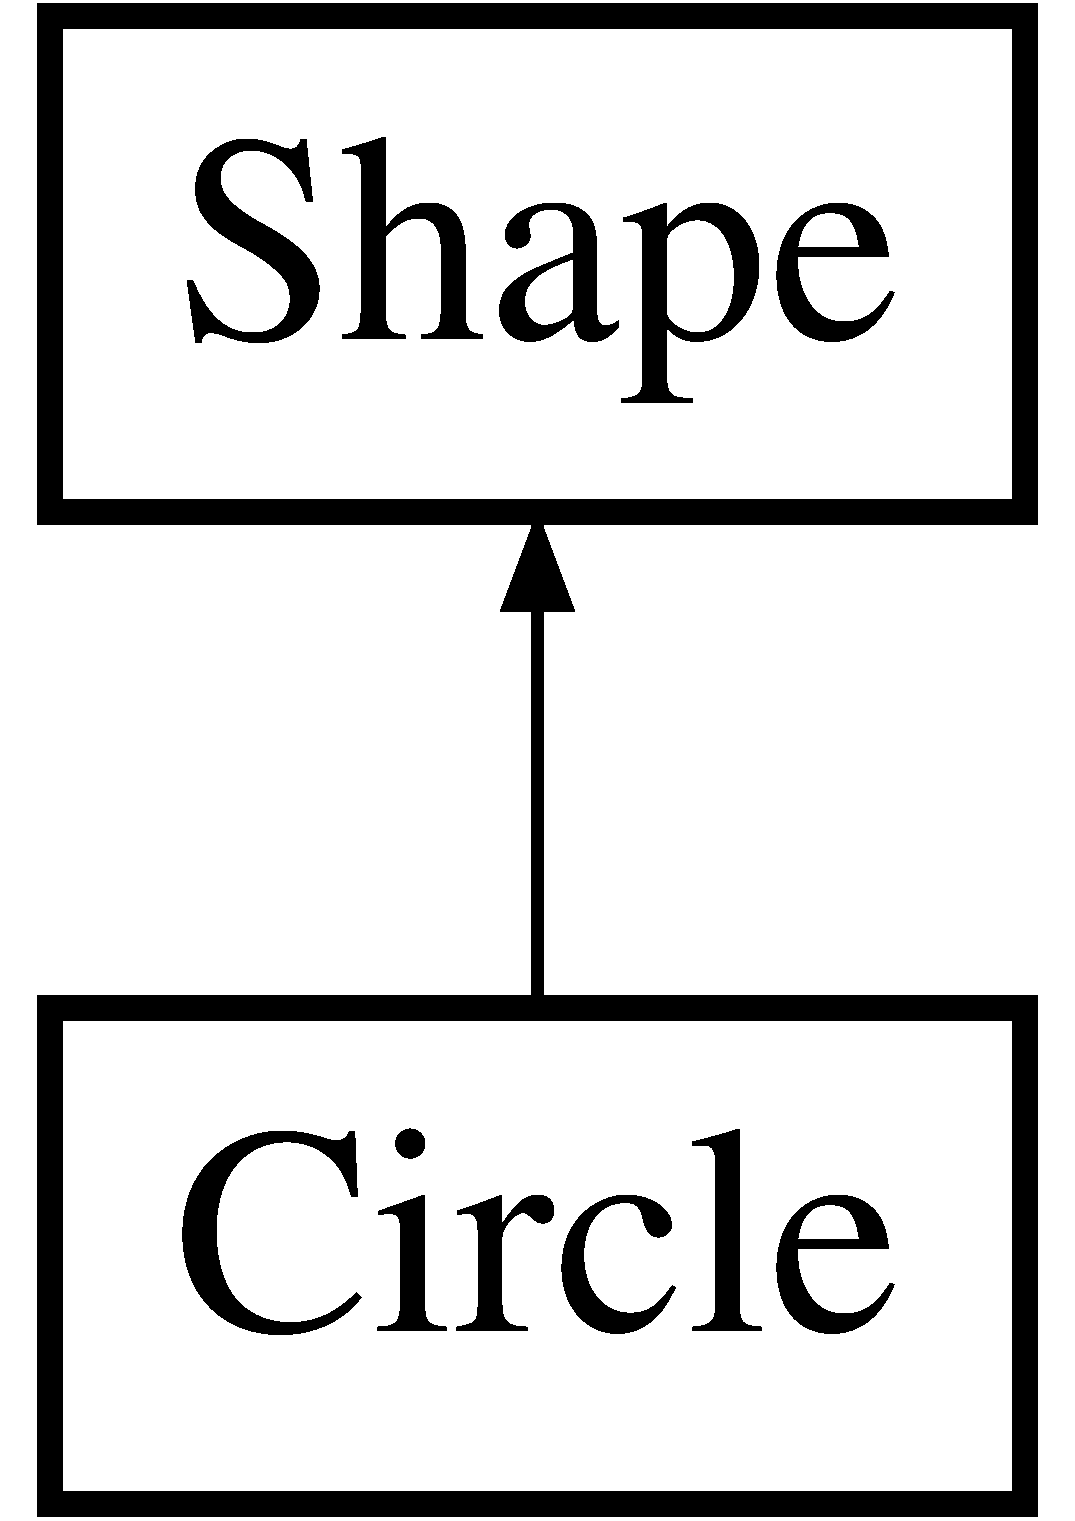
\includegraphics[height=2.000000cm]{class_circle}
\end{center}
\end{figure}
\subsection*{Public Member Functions}
\begin{DoxyCompactItemize}
\item 
\hyperlink{class_circle_ad1ecfcfc7bf34529c6a6d6c448bf70fe}{Circle} ()
\item 
\hyperlink{class_circle_ace551ce2e85abb8660f74ee34f5761a1}{Circle} (int \hyperlink{class_shape_a41e403e73d2949f1a6adfba6032c41ec}{x}, int \hyperlink{class_shape_ac757f715cc5b5681f2c691663ac06f0a}{y}, double \hyperlink{class_circle_addf06b37dda7589ade30e7ea21fe17be}{radius})
\item 
\hyperlink{class_circle_a05c707753451188c26b43508b610ff8e}{Circle} (double \hyperlink{class_circle_addf06b37dda7589ade30e7ea21fe17be}{radius})
\item 
string \hyperlink{class_circle_a3fcc66abd3f30a3c19e3bb63452fc2ed}{draw} () const 
\begin{DoxyCompactList}\small\item\em generate ps code for shape \end{DoxyCompactList}\item 
string \hyperlink{class_circle_a18f2b8aaa80fb870c3aea1798f32678b}{draw} (int \hyperlink{class_shape_a41e403e73d2949f1a6adfba6032c41ec}{x}, int \hyperlink{class_shape_ac757f715cc5b5681f2c691663ac06f0a}{y}) const 
\begin{DoxyCompactList}\small\item\em generate ps code for shape \end{DoxyCompactList}\item 
double \hyperlink{class_circle_addf06b37dda7589ade30e7ea21fe17be}{radius} ()
\begin{DoxyCompactList}\small\item\em returns radius \end{DoxyCompactList}\end{DoxyCompactItemize}
\subsection*{Protected Attributes}
\begin{DoxyCompactItemize}
\item 
double \hyperlink{class_circle_a7daf9293b23457177dbc0fadb960e07e}{radius\+\_\+}
\end{DoxyCompactItemize}


\subsection{Detailed Description}


Definition at line 14 of file circle.\+h.



\subsection{Constructor \& Destructor Documentation}
\hypertarget{class_circle_ad1ecfcfc7bf34529c6a6d6c448bf70fe}{}\index{Circle@{Circle}!Circle@{Circle}}
\index{Circle@{Circle}!Circle@{Circle}}
\subsubsection[{Circle()}]{\setlength{\rightskip}{0pt plus 5cm}Circle\+::\+Circle (
\begin{DoxyParamCaption}
{}
\end{DoxyParamCaption}
)\hspace{0.3cm}{\ttfamily [inline]}}\label{class_circle_ad1ecfcfc7bf34529c6a6d6c448bf70fe}


Definition at line 17 of file circle.\+h.

\hypertarget{class_circle_ace551ce2e85abb8660f74ee34f5761a1}{}\index{Circle@{Circle}!Circle@{Circle}}
\index{Circle@{Circle}!Circle@{Circle}}
\subsubsection[{Circle(int x, int y, double radius)}]{\setlength{\rightskip}{0pt plus 5cm}Circle\+::\+Circle (
\begin{DoxyParamCaption}
\item[{int}]{x, }
\item[{int}]{y, }
\item[{double}]{radius}
\end{DoxyParamCaption}
)\hspace{0.3cm}{\ttfamily [inline]}}\label{class_circle_ace551ce2e85abb8660f74ee34f5761a1}


Definition at line 18 of file circle.\+h.

\hypertarget{class_circle_a05c707753451188c26b43508b610ff8e}{}\index{Circle@{Circle}!Circle@{Circle}}
\index{Circle@{Circle}!Circle@{Circle}}
\subsubsection[{Circle(double radius)}]{\setlength{\rightskip}{0pt plus 5cm}Circle\+::\+Circle (
\begin{DoxyParamCaption}
\item[{double}]{radius}
\end{DoxyParamCaption}
)\hspace{0.3cm}{\ttfamily [inline]}}\label{class_circle_a05c707753451188c26b43508b610ff8e}


Definition at line 19 of file circle.\+h.



\subsection{Member Function Documentation}
\hypertarget{class_circle_a3fcc66abd3f30a3c19e3bb63452fc2ed}{}\index{Circle@{Circle}!draw@{draw}}
\index{draw@{draw}!Circle@{Circle}}
\subsubsection[{draw() const }]{\setlength{\rightskip}{0pt plus 5cm}string Circle\+::draw (
\begin{DoxyParamCaption}
{}
\end{DoxyParamCaption}
) const\hspace{0.3cm}{\ttfamily [virtual]}}\label{class_circle_a3fcc66abd3f30a3c19e3bb63452fc2ed}


generate ps code for shape 

generate ps code for drawing shape at default location \begin{DoxyReturn}{Returns}
string containing ps code for drawing shape at default location 
\end{DoxyReturn}


Reimplemented from \hyperlink{class_shape_a8405e352e8bbbdd173fd89065d63a80b}{Shape}.



Definition at line 15 of file circle.\+cpp.

\hypertarget{class_circle_a18f2b8aaa80fb870c3aea1798f32678b}{}\index{Circle@{Circle}!draw@{draw}}
\index{draw@{draw}!Circle@{Circle}}
\subsubsection[{draw(int x, int y) const }]{\setlength{\rightskip}{0pt plus 5cm}string Circle\+::draw (
\begin{DoxyParamCaption}
\item[{int}]{x, }
\item[{int}]{y}
\end{DoxyParamCaption}
) const\hspace{0.3cm}{\ttfamily [virtual]}}\label{class_circle_a18f2b8aaa80fb870c3aea1798f32678b}


generate ps code for shape 

generate ps code for drawing shape at specified coordinates


\begin{DoxyParams}{Parameters}
{\em x} & x position for center of shape\textquotesingle{}s desired location \\
\hline
{\em y} & y position for center of shape\textquotesingle{}s desired location\\
\hline
\end{DoxyParams}
\begin{DoxyReturn}{Returns}
string containing ps code for drawing shape at specified location 
\end{DoxyReturn}


Reimplemented from \hyperlink{class_shape_af26d06a96ece90a563795ec571451eb1}{Shape}.



Definition at line 19 of file circle.\+cpp.

\hypertarget{class_circle_addf06b37dda7589ade30e7ea21fe17be}{}\index{Circle@{Circle}!radius@{radius}}
\index{radius@{radius}!Circle@{Circle}}
\subsubsection[{radius()}]{\setlength{\rightskip}{0pt plus 5cm}double Circle\+::radius (
\begin{DoxyParamCaption}
{}
\end{DoxyParamCaption}
)\hspace{0.3cm}{\ttfamily [virtual]}}\label{class_circle_addf06b37dda7589ade30e7ea21fe17be}


returns radius 

returns the radius of a shape, only defined for \hyperlink{class_polygon}{Polygon} and \hyperlink{class_circle}{Circle} \begin{DoxyReturn}{Returns}
if \hyperlink{class_polygon}{Polygon} or \hyperlink{class_circle}{Circle}, returns the radius. Otherwise returns 0. 
\end{DoxyReturn}


Reimplemented from \hyperlink{class_shape_a8193b252afa84bbf0b173160d2b3302d}{Shape}.



Definition at line 11 of file circle.\+cpp.



\subsection{Member Data Documentation}
\hypertarget{class_circle_a7daf9293b23457177dbc0fadb960e07e}{}\index{Circle@{Circle}!radius\+\_\+@{radius\+\_\+}}
\index{radius\+\_\+@{radius\+\_\+}!Circle@{Circle}}
\subsubsection[{radius\+\_\+}]{\setlength{\rightskip}{0pt plus 5cm}double Circle\+::radius\+\_\+\hspace{0.3cm}{\ttfamily [protected]}}\label{class_circle_a7daf9293b23457177dbc0fadb960e07e}
radius of circle 

Definition at line 30 of file circle.\+h.



The documentation for this class was generated from the following files\+:\begin{DoxyCompactItemize}
\item 
\hyperlink{circle_8h}{circle.\+h}\item 
\hyperlink{circle_8cpp}{circle.\+cpp}\end{DoxyCompactItemize}

\hypertarget{class_horizontal}{}\section{Horizontal Class Reference}
\label{class_horizontal}\index{Horizontal@{Horizontal}}


{\ttfamily \#include $<$layered.\+h$>$}

Inheritance diagram for Horizontal\+:\begin{figure}[H]
\begin{center}
\leavevmode
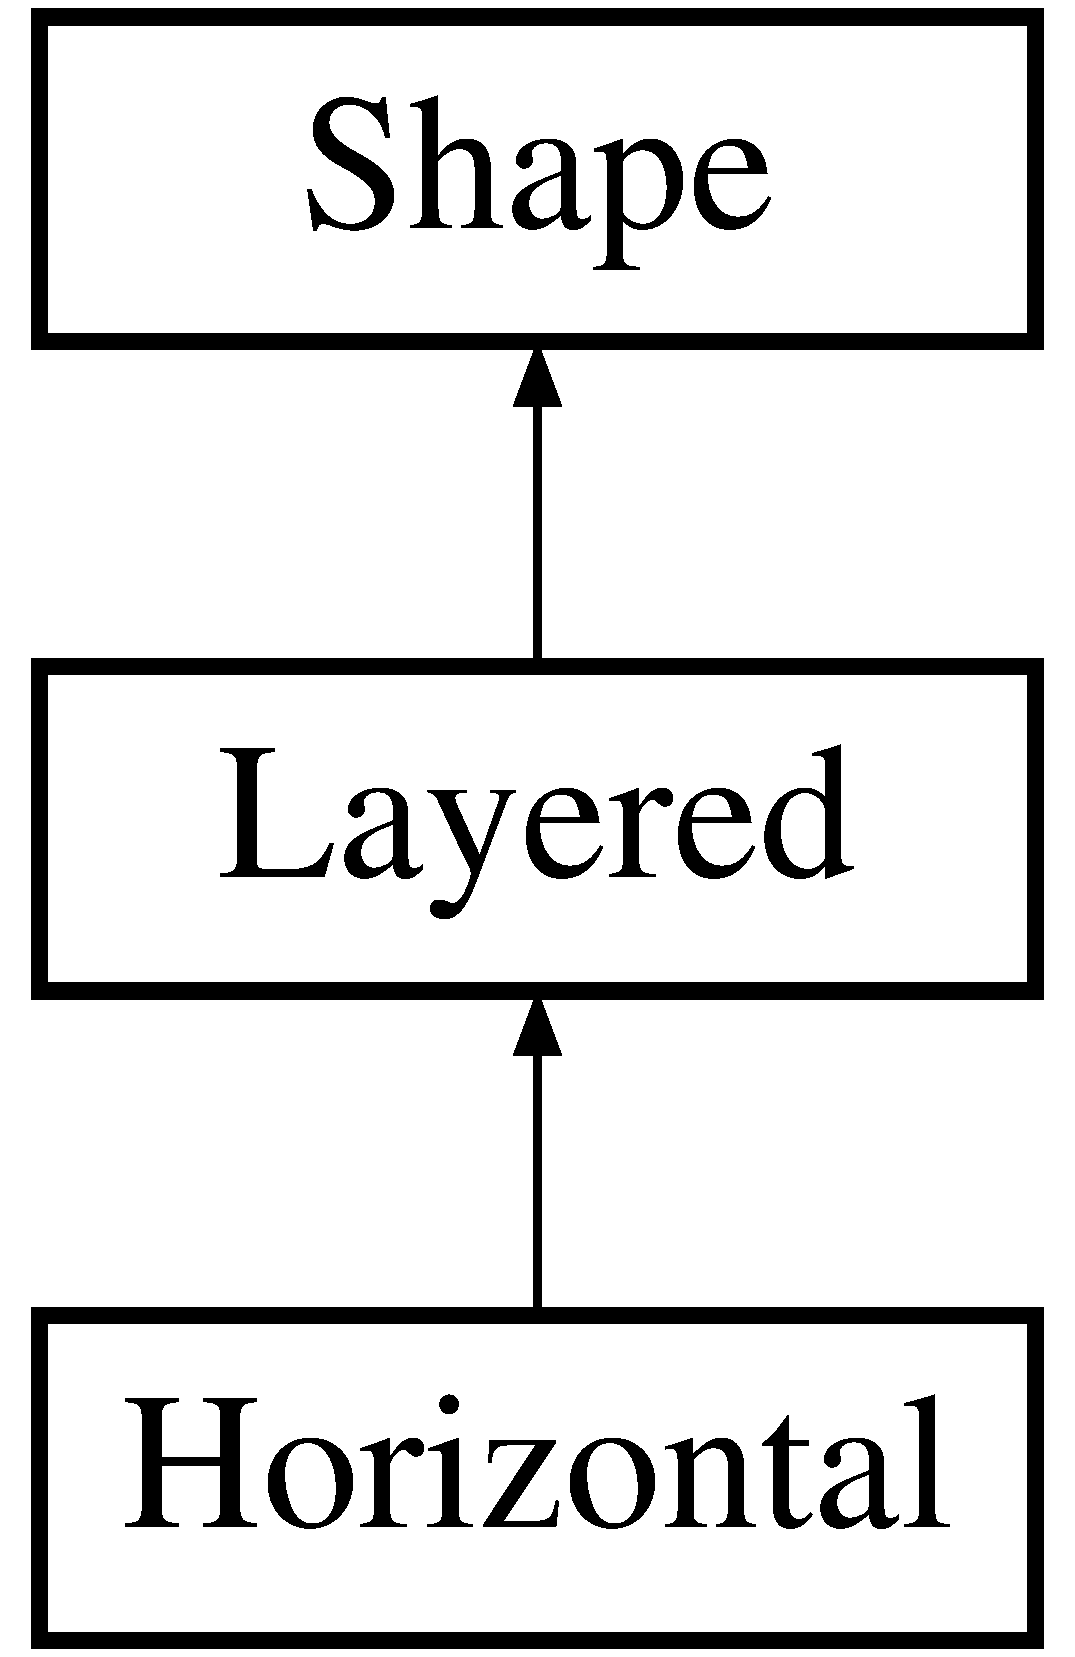
\includegraphics[height=3.000000cm]{class_horizontal}
\end{center}
\end{figure}
\subsection*{Public Member Functions}
\begin{DoxyCompactItemize}
\item 
\hyperlink{class_horizontal_a21ca6396569c657e9f6e16f07c9d0eec}{Horizontal} ()
\item 
\hyperlink{class_horizontal_a2f0a00cf0c24b1e5f001a315901274b0}{Horizontal} (int \hyperlink{class_shape_a41e403e73d2949f1a6adfba6032c41ec}{x}, int \hyperlink{class_shape_ac757f715cc5b5681f2c691663ac06f0a}{y}, initializer\+\_\+list$<$ \hyperlink{class_shape}{Shape} $\ast$ $>$ shapes)
\begin{DoxyCompactList}\small\item\em \hyperlink{class_horizontal}{Horizontal} costructor. \end{DoxyCompactList}\item 
\hyperlink{class_horizontal_a640dc2d55b1ba908b7eecff612b4e147}{Horizontal} (initializer\+\_\+list$<$ \hyperlink{class_shape}{Shape} $\ast$ $>$ shapes)
\item 
string \hyperlink{class_horizontal_a79e26b6d0db2a2b7e4f25a3f0f67e7a2}{draw} () const 
\begin{DoxyCompactList}\small\item\em generate ps code for shape \end{DoxyCompactList}\item 
string \hyperlink{class_horizontal_aea100857d1a9a269b66060b8bd32ced1}{draw} (int \hyperlink{class_shape_a41e403e73d2949f1a6adfba6032c41ec}{x}, int \hyperlink{class_shape_ac757f715cc5b5681f2c691663ac06f0a}{y}) const 
\begin{DoxyCompactList}\small\item\em generate ps code for shape \end{DoxyCompactList}\end{DoxyCompactItemize}
\subsection*{Additional Inherited Members}


\subsection{Detailed Description}


Definition at line 35 of file layered.\+h.



\subsection{Constructor \& Destructor Documentation}
\hypertarget{class_horizontal_a21ca6396569c657e9f6e16f07c9d0eec}{}\index{Horizontal@{Horizontal}!Horizontal@{Horizontal}}
\index{Horizontal@{Horizontal}!Horizontal@{Horizontal}}
\subsubsection[{Horizontal()}]{\setlength{\rightskip}{0pt plus 5cm}Horizontal\+::\+Horizontal (
\begin{DoxyParamCaption}
{}
\end{DoxyParamCaption}
)\hspace{0.3cm}{\ttfamily [inline]}}\label{class_horizontal_a21ca6396569c657e9f6e16f07c9d0eec}


Definition at line 38 of file layered.\+h.

\hypertarget{class_horizontal_a2f0a00cf0c24b1e5f001a315901274b0}{}\index{Horizontal@{Horizontal}!Horizontal@{Horizontal}}
\index{Horizontal@{Horizontal}!Horizontal@{Horizontal}}
\subsubsection[{Horizontal(int x, int y, initializer\+\_\+list$<$ Shape $\ast$ $>$ shapes)}]{\setlength{\rightskip}{0pt plus 5cm}Horizontal\+::\+Horizontal (
\begin{DoxyParamCaption}
\item[{int}]{x, }
\item[{int}]{y, }
\item[{initializer\+\_\+list$<$ {\bf Shape} $\ast$ $>$}]{shapes}
\end{DoxyParamCaption}
)}\label{class_horizontal_a2f0a00cf0c24b1e5f001a315901274b0}


\hyperlink{class_horizontal}{Horizontal} costructor. 

constructs a \hyperlink{class_horizontal}{Horizontal} shape from a list of Shapes


\begin{DoxyParams}{Parameters}
{\em x} & x position of center \\
\hline
{\em y} & y position of center \\
\hline
{\em shapes} & list of pointers to Shapes \\
\hline
\end{DoxyParams}


Definition at line 55 of file layered.\+cpp.

\hypertarget{class_horizontal_a640dc2d55b1ba908b7eecff612b4e147}{}\index{Horizontal@{Horizontal}!Horizontal@{Horizontal}}
\index{Horizontal@{Horizontal}!Horizontal@{Horizontal}}
\subsubsection[{Horizontal(initializer\+\_\+list$<$ Shape $\ast$ $>$ shapes)}]{\setlength{\rightskip}{0pt plus 5cm}Horizontal\+::\+Horizontal (
\begin{DoxyParamCaption}
\item[{initializer\+\_\+list$<$ {\bf Shape} $\ast$ $>$}]{shapes}
\end{DoxyParamCaption}
)\hspace{0.3cm}{\ttfamily [inline]}}\label{class_horizontal_a640dc2d55b1ba908b7eecff612b4e147}


Definition at line 40 of file layered.\+h.



\subsection{Member Function Documentation}
\hypertarget{class_horizontal_a79e26b6d0db2a2b7e4f25a3f0f67e7a2}{}\index{Horizontal@{Horizontal}!draw@{draw}}
\index{draw@{draw}!Horizontal@{Horizontal}}
\subsubsection[{draw() const }]{\setlength{\rightskip}{0pt plus 5cm}string Horizontal\+::draw (
\begin{DoxyParamCaption}
{}
\end{DoxyParamCaption}
) const\hspace{0.3cm}{\ttfamily [virtual]}}\label{class_horizontal_a79e26b6d0db2a2b7e4f25a3f0f67e7a2}


generate ps code for shape 

generate ps code for drawing shape at default location \begin{DoxyReturn}{Returns}
string containing ps code for drawing shape at default location 
\end{DoxyReturn}


Reimplemented from \hyperlink{class_layered_a968cd141e61eb039b997352a318dcae0}{Layered}.



Definition at line 65 of file layered.\+cpp.

\hypertarget{class_horizontal_aea100857d1a9a269b66060b8bd32ced1}{}\index{Horizontal@{Horizontal}!draw@{draw}}
\index{draw@{draw}!Horizontal@{Horizontal}}
\subsubsection[{draw(int x, int y) const }]{\setlength{\rightskip}{0pt plus 5cm}string Horizontal\+::draw (
\begin{DoxyParamCaption}
\item[{int}]{x, }
\item[{int}]{y}
\end{DoxyParamCaption}
) const\hspace{0.3cm}{\ttfamily [virtual]}}\label{class_horizontal_aea100857d1a9a269b66060b8bd32ced1}


generate ps code for shape 

generate ps code for drawing shape at specified coordinates


\begin{DoxyParams}{Parameters}
{\em x} & x position for center of shape\textquotesingle{}s desired location \\
\hline
{\em y} & y position for center of shape\textquotesingle{}s desired location\\
\hline
\end{DoxyParams}
\begin{DoxyReturn}{Returns}
string containing ps code for drawing shape at specified location 
\end{DoxyReturn}


Reimplemented from \hyperlink{class_layered_a6eb564ff0646b26fdd4175856b1a0815}{Layered}.



Definition at line 69 of file layered.\+cpp.



The documentation for this class was generated from the following files\+:\begin{DoxyCompactItemize}
\item 
\hyperlink{layered_8h}{layered.\+h}\item 
\hyperlink{layered_8cpp}{layered.\+cpp}\end{DoxyCompactItemize}

\hypertarget{class_layered}{}\section{Layered Class Reference}
\label{class_layered}\index{Layered@{Layered}}


{\ttfamily \#include $<$layered.\+h$>$}

Inheritance diagram for Layered\+:\begin{figure}[H]
\begin{center}
\leavevmode
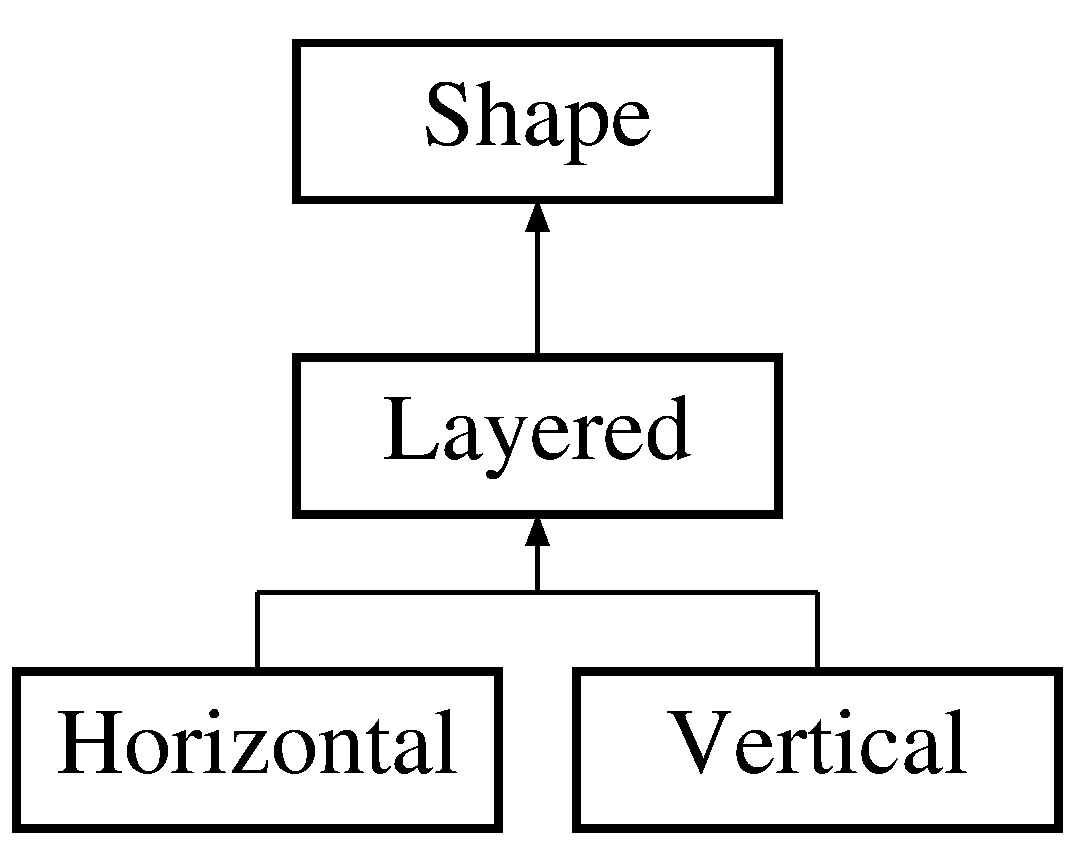
\includegraphics[height=3.000000cm]{class_layered}
\end{center}
\end{figure}
\subsection*{Public Member Functions}
\begin{DoxyCompactItemize}
\item 
\hyperlink{class_layered_a6a9d25d4d62c7dc21f93b8384c4f91ce}{Layered} ()
\item 
\hyperlink{class_layered_a5957ef351efc54bcfe38719b3ef5e1a4}{Layered} (int \hyperlink{class_shape_a41e403e73d2949f1a6adfba6032c41ec}{x}, int \hyperlink{class_shape_ac757f715cc5b5681f2c691663ac06f0a}{y}, initializer\+\_\+list$<$ \hyperlink{class_shape}{Shape} $\ast$ $>$ shapes)
\begin{DoxyCompactList}\small\item\em \hyperlink{class_layered}{Layered} constructor. \end{DoxyCompactList}\item 
\hyperlink{class_layered_ac9c58b109dfc7204a3a4be1a185cb1f2}{Layered} (initializer\+\_\+list$<$ \hyperlink{class_shape}{Shape} $\ast$ $>$ shapes)
\item 
string \hyperlink{class_layered_a968cd141e61eb039b997352a318dcae0}{draw} () const 
\begin{DoxyCompactList}\small\item\em generate ps code for shape \end{DoxyCompactList}\item 
string \hyperlink{class_layered_a6eb564ff0646b26fdd4175856b1a0815}{draw} (int \hyperlink{class_shape_a41e403e73d2949f1a6adfba6032c41ec}{x}, int \hyperlink{class_shape_ac757f715cc5b5681f2c691663ac06f0a}{y}) const 
\begin{DoxyCompactList}\small\item\em generate ps code for shape \end{DoxyCompactList}\end{DoxyCompactItemize}
\subsection*{Protected Attributes}
\begin{DoxyCompactItemize}
\item 
initializer\+\_\+list$<$ \hyperlink{class_shape}{Shape} $\ast$ $>$ \hyperlink{class_layered_a80ab4f9aaec1246a9d16400bbf8d3dce}{shapes\+\_\+}
\end{DoxyCompactItemize}


\subsection{Detailed Description}


Definition at line 17 of file layered.\+h.



\subsection{Constructor \& Destructor Documentation}
\hypertarget{class_layered_a6a9d25d4d62c7dc21f93b8384c4f91ce}{}\index{Layered@{Layered}!Layered@{Layered}}
\index{Layered@{Layered}!Layered@{Layered}}
\subsubsection[{Layered()}]{\setlength{\rightskip}{0pt plus 5cm}Layered\+::\+Layered (
\begin{DoxyParamCaption}
{}
\end{DoxyParamCaption}
)\hspace{0.3cm}{\ttfamily [inline]}}\label{class_layered_a6a9d25d4d62c7dc21f93b8384c4f91ce}


Definition at line 20 of file layered.\+h.

\hypertarget{class_layered_a5957ef351efc54bcfe38719b3ef5e1a4}{}\index{Layered@{Layered}!Layered@{Layered}}
\index{Layered@{Layered}!Layered@{Layered}}
\subsubsection[{Layered(int x, int y, initializer\+\_\+list$<$ Shape $\ast$ $>$ shapes)}]{\setlength{\rightskip}{0pt plus 5cm}Layered\+::\+Layered (
\begin{DoxyParamCaption}
\item[{int}]{x, }
\item[{int}]{y, }
\item[{initializer\+\_\+list$<$ {\bf Shape} $\ast$ $>$}]{shapes}
\end{DoxyParamCaption}
)}\label{class_layered_a5957ef351efc54bcfe38719b3ef5e1a4}


\hyperlink{class_layered}{Layered} constructor. 

constructs a \hyperlink{class_layered}{Layered} shape from a list of shapes


\begin{DoxyParams}{Parameters}
{\em x} & x position of center \\
\hline
{\em y} & y position of center \\
\hline
{\em shapes} & list of pointers to Shapes \\
\hline
\end{DoxyParams}


Definition at line 19 of file layered.\+cpp.

\hypertarget{class_layered_ac9c58b109dfc7204a3a4be1a185cb1f2}{}\index{Layered@{Layered}!Layered@{Layered}}
\index{Layered@{Layered}!Layered@{Layered}}
\subsubsection[{Layered(initializer\+\_\+list$<$ Shape $\ast$ $>$ shapes)}]{\setlength{\rightskip}{0pt plus 5cm}Layered\+::\+Layered (
\begin{DoxyParamCaption}
\item[{initializer\+\_\+list$<$ {\bf Shape} $\ast$ $>$}]{shapes}
\end{DoxyParamCaption}
)\hspace{0.3cm}{\ttfamily [inline]}}\label{class_layered_ac9c58b109dfc7204a3a4be1a185cb1f2}


Definition at line 22 of file layered.\+h.



\subsection{Member Function Documentation}
\hypertarget{class_layered_a968cd141e61eb039b997352a318dcae0}{}\index{Layered@{Layered}!draw@{draw}}
\index{draw@{draw}!Layered@{Layered}}
\subsubsection[{draw() const }]{\setlength{\rightskip}{0pt plus 5cm}string Layered\+::draw (
\begin{DoxyParamCaption}
{}
\end{DoxyParamCaption}
) const\hspace{0.3cm}{\ttfamily [virtual]}}\label{class_layered_a968cd141e61eb039b997352a318dcae0}


generate ps code for shape 

generate ps code for drawing shape at default location \begin{DoxyReturn}{Returns}
string containing ps code for drawing shape at default location 
\end{DoxyReturn}


Reimplemented from \hyperlink{class_shape_a8405e352e8bbbdd173fd89065d63a80b}{Shape}.



Reimplemented in \hyperlink{class_vertical_a778fd2aa48afcf255b75413e29613ebb}{Vertical}, and \hyperlink{class_horizontal_a79e26b6d0db2a2b7e4f25a3f0f67e7a2}{Horizontal}.



Definition at line 29 of file layered.\+cpp.

\hypertarget{class_layered_a6eb564ff0646b26fdd4175856b1a0815}{}\index{Layered@{Layered}!draw@{draw}}
\index{draw@{draw}!Layered@{Layered}}
\subsubsection[{draw(int x, int y) const }]{\setlength{\rightskip}{0pt plus 5cm}string Layered\+::draw (
\begin{DoxyParamCaption}
\item[{int}]{x, }
\item[{int}]{y}
\end{DoxyParamCaption}
) const\hspace{0.3cm}{\ttfamily [virtual]}}\label{class_layered_a6eb564ff0646b26fdd4175856b1a0815}


generate ps code for shape 

generate ps code for drawing shape at specified coordinates


\begin{DoxyParams}{Parameters}
{\em x} & x position for center of shape\textquotesingle{}s desired location \\
\hline
{\em y} & y position for center of shape\textquotesingle{}s desired location\\
\hline
\end{DoxyParams}
\begin{DoxyReturn}{Returns}
string containing ps code for drawing shape at specified location 
\end{DoxyReturn}


Reimplemented from \hyperlink{class_shape_af26d06a96ece90a563795ec571451eb1}{Shape}.



Reimplemented in \hyperlink{class_vertical_a9be329f986230ccaa35ec7f63553d658}{Vertical}, and \hyperlink{class_horizontal_aea100857d1a9a269b66060b8bd32ced1}{Horizontal}.



Definition at line 33 of file layered.\+cpp.



\subsection{Member Data Documentation}
\hypertarget{class_layered_a80ab4f9aaec1246a9d16400bbf8d3dce}{}\index{Layered@{Layered}!shapes\+\_\+@{shapes\+\_\+}}
\index{shapes\+\_\+@{shapes\+\_\+}!Layered@{Layered}}
\subsubsection[{shapes\+\_\+}]{\setlength{\rightskip}{0pt plus 5cm}initializer\+\_\+list$<${\bf Shape}$\ast$$>$ Layered\+::shapes\+\_\+\hspace{0.3cm}{\ttfamily [protected]}}\label{class_layered_a80ab4f9aaec1246a9d16400bbf8d3dce}
vector of pointers to \hyperlink{class_shape}{Shape} objects 

Definition at line 31 of file layered.\+h.



The documentation for this class was generated from the following files\+:\begin{DoxyCompactItemize}
\item 
\hyperlink{layered_8h}{layered.\+h}\item 
\hyperlink{layered_8cpp}{layered.\+cpp}\end{DoxyCompactItemize}

\hypertarget{class_polygon}{}\section{Polygon Class Reference}
\label{class_polygon}\index{Polygon@{Polygon}}


{\ttfamily \#include $<$polygon.\+h$>$}

Inheritance diagram for Polygon\+:\begin{figure}[H]
\begin{center}
\leavevmode
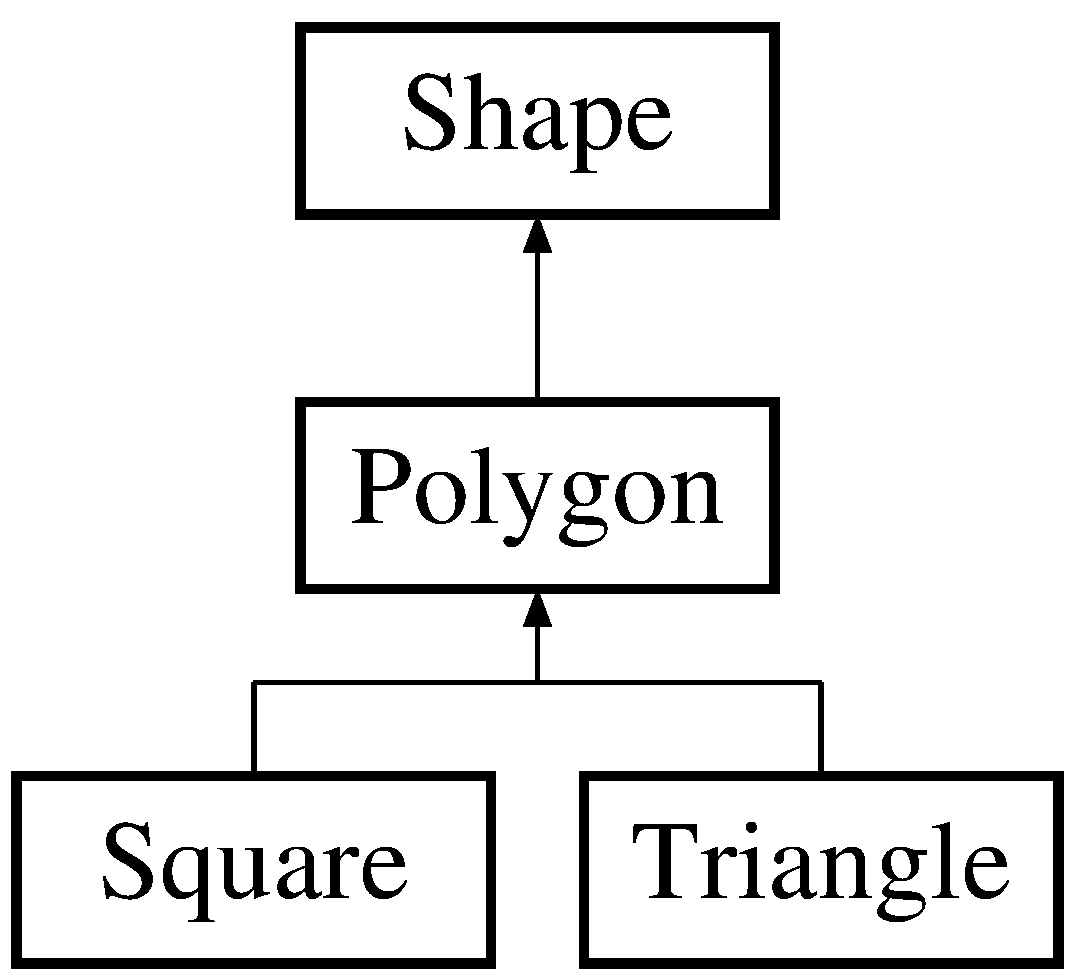
\includegraphics[height=3.000000cm]{class_polygon}
\end{center}
\end{figure}
\subsection*{Public Member Functions}
\begin{DoxyCompactItemize}
\item 
\hyperlink{class_polygon_ac183e712f8be1e13f1c9d5b4d4512ead}{Polygon} ()
\item 
\hyperlink{class_polygon_a295d10cfffd80d67f603642d82f62279}{Polygon} (int \hyperlink{class_shape_a41e403e73d2949f1a6adfba6032c41ec}{x}, int \hyperlink{class_shape_ac757f715cc5b5681f2c691663ac06f0a}{y}, int sides, double length)
\item 
\hyperlink{class_polygon_a8cb36a982609ea22b8722b76cfa9d6fa}{Polygon} (int sides, double length)
\item 
string \hyperlink{class_polygon_a732b40203a5cc2baadd90446c3ec8213}{draw} () const 
\begin{DoxyCompactList}\small\item\em generates ps code for drawing a polygon \end{DoxyCompactList}\item 
string \hyperlink{class_polygon_af0f4e693010935528bb3e99bca2cc433}{draw} (int \hyperlink{class_shape_a41e403e73d2949f1a6adfba6032c41ec}{x}, int \hyperlink{class_shape_ac757f715cc5b5681f2c691663ac06f0a}{y}) const 
\begin{DoxyCompactList}\small\item\em generates ps code for drawing a polygon \end{DoxyCompactList}\item 
int \hyperlink{class_polygon_a3c57ca9893bf151501123b8b1787acf6}{num\+Of\+Sides} ()
\begin{DoxyCompactList}\small\item\em returns number of sides \end{DoxyCompactList}\item 
double \hyperlink{class_polygon_ab03b3c38a9f26b2c0d46294dd77f4318}{side\+Length} ()
\begin{DoxyCompactList}\small\item\em returns side length \end{DoxyCompactList}\item 
double \hyperlink{class_polygon_af1af4ce31b24eb31b4300e932f2578c2}{radius} ()
\begin{DoxyCompactList}\small\item\em returns radius \end{DoxyCompactList}\end{DoxyCompactItemize}
\subsection*{Protected Attributes}
\begin{DoxyCompactItemize}
\item 
int \hyperlink{class_polygon_a2c2596c34f01b275323971f8f29e4cd5}{num\+Of\+Sides\+\_\+}
\item 
double \hyperlink{class_polygon_a22a65792492ceb172e3f9ac63a619864}{side\+Length\+\_\+}
\item 
double \hyperlink{class_polygon_ae9ee97d51db108f9e2cc073aabaa68df}{radius\+\_\+}
\end{DoxyCompactItemize}


\subsection{Detailed Description}


Definition at line 14 of file polygon.\+h.



\subsection{Constructor \& Destructor Documentation}
\hypertarget{class_polygon_ac183e712f8be1e13f1c9d5b4d4512ead}{}\index{Polygon@{Polygon}!Polygon@{Polygon}}
\index{Polygon@{Polygon}!Polygon@{Polygon}}
\subsubsection[{Polygon()}]{\setlength{\rightskip}{0pt plus 5cm}Polygon\+::\+Polygon (
\begin{DoxyParamCaption}
{}
\end{DoxyParamCaption}
)\hspace{0.3cm}{\ttfamily [inline]}}\label{class_polygon_ac183e712f8be1e13f1c9d5b4d4512ead}


Definition at line 17 of file polygon.\+h.

\hypertarget{class_polygon_a295d10cfffd80d67f603642d82f62279}{}\index{Polygon@{Polygon}!Polygon@{Polygon}}
\index{Polygon@{Polygon}!Polygon@{Polygon}}
\subsubsection[{Polygon(int x, int y, int sides, double length)}]{\setlength{\rightskip}{0pt plus 5cm}Polygon\+::\+Polygon (
\begin{DoxyParamCaption}
\item[{int}]{x, }
\item[{int}]{y, }
\item[{int}]{sides, }
\item[{double}]{length}
\end{DoxyParamCaption}
)\hspace{0.3cm}{\ttfamily [inline]}}\label{class_polygon_a295d10cfffd80d67f603642d82f62279}


Definition at line 24 of file polygon.\+h.

\hypertarget{class_polygon_a8cb36a982609ea22b8722b76cfa9d6fa}{}\index{Polygon@{Polygon}!Polygon@{Polygon}}
\index{Polygon@{Polygon}!Polygon@{Polygon}}
\subsubsection[{Polygon(int sides, double length)}]{\setlength{\rightskip}{0pt plus 5cm}Polygon\+::\+Polygon (
\begin{DoxyParamCaption}
\item[{int}]{sides, }
\item[{double}]{length}
\end{DoxyParamCaption}
)\hspace{0.3cm}{\ttfamily [inline]}}\label{class_polygon_a8cb36a982609ea22b8722b76cfa9d6fa}


Definition at line 31 of file polygon.\+h.



\subsection{Member Function Documentation}
\hypertarget{class_polygon_a732b40203a5cc2baadd90446c3ec8213}{}\index{Polygon@{Polygon}!draw@{draw}}
\index{draw@{draw}!Polygon@{Polygon}}
\subsubsection[{draw() const }]{\setlength{\rightskip}{0pt plus 5cm}string Polygon\+::draw (
\begin{DoxyParamCaption}
{}
\end{DoxyParamCaption}
) const\hspace{0.3cm}{\ttfamily [virtual]}}\label{class_polygon_a732b40203a5cc2baadd90446c3ec8213}


generates ps code for drawing a polygon 

returns a string containing the ps code for drawing any equilateral polygon \begin{DoxyReturn}{Returns}
string containing ps code 
\end{DoxyReturn}


Reimplemented from \hyperlink{class_shape_a8405e352e8bbbdd173fd89065d63a80b}{Shape}.



Definition at line 16 of file polygon.\+cpp.

\hypertarget{class_polygon_af0f4e693010935528bb3e99bca2cc433}{}\index{Polygon@{Polygon}!draw@{draw}}
\index{draw@{draw}!Polygon@{Polygon}}
\subsubsection[{draw(int x, int y) const }]{\setlength{\rightskip}{0pt plus 5cm}string Polygon\+::draw (
\begin{DoxyParamCaption}
\item[{int}]{x, }
\item[{int}]{y}
\end{DoxyParamCaption}
) const\hspace{0.3cm}{\ttfamily [virtual]}}\label{class_polygon_af0f4e693010935528bb3e99bca2cc433}


generates ps code for drawing a polygon 

returns a string containing the ps code for drawing any equilateral polygon


\begin{DoxyParams}{Parameters}
{\em x} & x position of center \\
\hline
{\em y} & y position of center\\
\hline
\end{DoxyParams}
\begin{DoxyReturn}{Returns}
string containing ps code 
\end{DoxyReturn}


Reimplemented from \hyperlink{class_shape_af26d06a96ece90a563795ec571451eb1}{Shape}.



Definition at line 30 of file polygon.\+cpp.

\hypertarget{class_polygon_a3c57ca9893bf151501123b8b1787acf6}{}\index{Polygon@{Polygon}!num\+Of\+Sides@{num\+Of\+Sides}}
\index{num\+Of\+Sides@{num\+Of\+Sides}!Polygon@{Polygon}}
\subsubsection[{num\+Of\+Sides()}]{\setlength{\rightskip}{0pt plus 5cm}int Polygon\+::num\+Of\+Sides (
\begin{DoxyParamCaption}
{}
\end{DoxyParamCaption}
)\hspace{0.3cm}{\ttfamily [virtual]}}\label{class_polygon_a3c57ca9893bf151501123b8b1787acf6}


returns number of sides 

returns number of sides of a shape, only defined for \hyperlink{class_polygon}{Polygon} \begin{DoxyReturn}{Returns}
if \hyperlink{class_polygon}{Polygon}, returns number of sides. Otherwise returns 0. 
\end{DoxyReturn}


Reimplemented from \hyperlink{class_shape_ac152ef6b8150122e1e279e3ac2d9b627}{Shape}.



Definition at line 50 of file polygon.\+cpp.

\hypertarget{class_polygon_af1af4ce31b24eb31b4300e932f2578c2}{}\index{Polygon@{Polygon}!radius@{radius}}
\index{radius@{radius}!Polygon@{Polygon}}
\subsubsection[{radius()}]{\setlength{\rightskip}{0pt plus 5cm}double Polygon\+::radius (
\begin{DoxyParamCaption}
{}
\end{DoxyParamCaption}
)\hspace{0.3cm}{\ttfamily [virtual]}}\label{class_polygon_af1af4ce31b24eb31b4300e932f2578c2}


returns radius 

returns the radius of a shape, only defined for \hyperlink{class_polygon}{Polygon} and \hyperlink{class_circle}{Circle} \begin{DoxyReturn}{Returns}
if \hyperlink{class_polygon}{Polygon} or \hyperlink{class_circle}{Circle}, returns the radius. Otherwise returns 0. 
\end{DoxyReturn}


Reimplemented from \hyperlink{class_shape_a8193b252afa84bbf0b173160d2b3302d}{Shape}.



Definition at line 56 of file polygon.\+cpp.

\hypertarget{class_polygon_ab03b3c38a9f26b2c0d46294dd77f4318}{}\index{Polygon@{Polygon}!side\+Length@{side\+Length}}
\index{side\+Length@{side\+Length}!Polygon@{Polygon}}
\subsubsection[{side\+Length()}]{\setlength{\rightskip}{0pt plus 5cm}double Polygon\+::side\+Length (
\begin{DoxyParamCaption}
{}
\end{DoxyParamCaption}
)\hspace{0.3cm}{\ttfamily [virtual]}}\label{class_polygon_ab03b3c38a9f26b2c0d46294dd77f4318}


returns side length 

returns length of a side of a shape, only defined for \hyperlink{class_polygon}{Polygon} \begin{DoxyReturn}{Returns}
if \hyperlink{class_polygon}{Polygon}, returns length of a side. Otherwise returns 0. 
\end{DoxyReturn}


Reimplemented from \hyperlink{class_shape_a116897479aa63aeea80648b7ac9e114a}{Shape}.



Definition at line 53 of file polygon.\+cpp.



\subsection{Member Data Documentation}
\hypertarget{class_polygon_a2c2596c34f01b275323971f8f29e4cd5}{}\index{Polygon@{Polygon}!num\+Of\+Sides\+\_\+@{num\+Of\+Sides\+\_\+}}
\index{num\+Of\+Sides\+\_\+@{num\+Of\+Sides\+\_\+}!Polygon@{Polygon}}
\subsubsection[{num\+Of\+Sides\+\_\+}]{\setlength{\rightskip}{0pt plus 5cm}int Polygon\+::num\+Of\+Sides\+\_\+\hspace{0.3cm}{\ttfamily [protected]}}\label{class_polygon_a2c2596c34f01b275323971f8f29e4cd5}
number of sides of the polygon 

Definition at line 46 of file polygon.\+h.

\hypertarget{class_polygon_ae9ee97d51db108f9e2cc073aabaa68df}{}\index{Polygon@{Polygon}!radius\+\_\+@{radius\+\_\+}}
\index{radius\+\_\+@{radius\+\_\+}!Polygon@{Polygon}}
\subsubsection[{radius\+\_\+}]{\setlength{\rightskip}{0pt plus 5cm}double Polygon\+::radius\+\_\+\hspace{0.3cm}{\ttfamily [protected]}}\label{class_polygon_ae9ee97d51db108f9e2cc073aabaa68df}
radius of polygon 

Definition at line 54 of file polygon.\+h.

\hypertarget{class_polygon_a22a65792492ceb172e3f9ac63a619864}{}\index{Polygon@{Polygon}!side\+Length\+\_\+@{side\+Length\+\_\+}}
\index{side\+Length\+\_\+@{side\+Length\+\_\+}!Polygon@{Polygon}}
\subsubsection[{side\+Length\+\_\+}]{\setlength{\rightskip}{0pt plus 5cm}double Polygon\+::side\+Length\+\_\+\hspace{0.3cm}{\ttfamily [protected]}}\label{class_polygon_a22a65792492ceb172e3f9ac63a619864}
length of polygon\textquotesingle{}s sides 

Definition at line 50 of file polygon.\+h.



The documentation for this class was generated from the following files\+:\begin{DoxyCompactItemize}
\item 
\hyperlink{polygon_8h}{polygon.\+h}\item 
\hyperlink{polygon_8cpp}{polygon.\+cpp}\end{DoxyCompactItemize}

\hypertarget{class_rectangle}{}\section{Rectangle Class Reference}
\label{class_rectangle}\index{Rectangle@{Rectangle}}


{\ttfamily \#include $<$rectangle.\+h$>$}

Inheritance diagram for Rectangle\+:\begin{figure}[H]
\begin{center}
\leavevmode
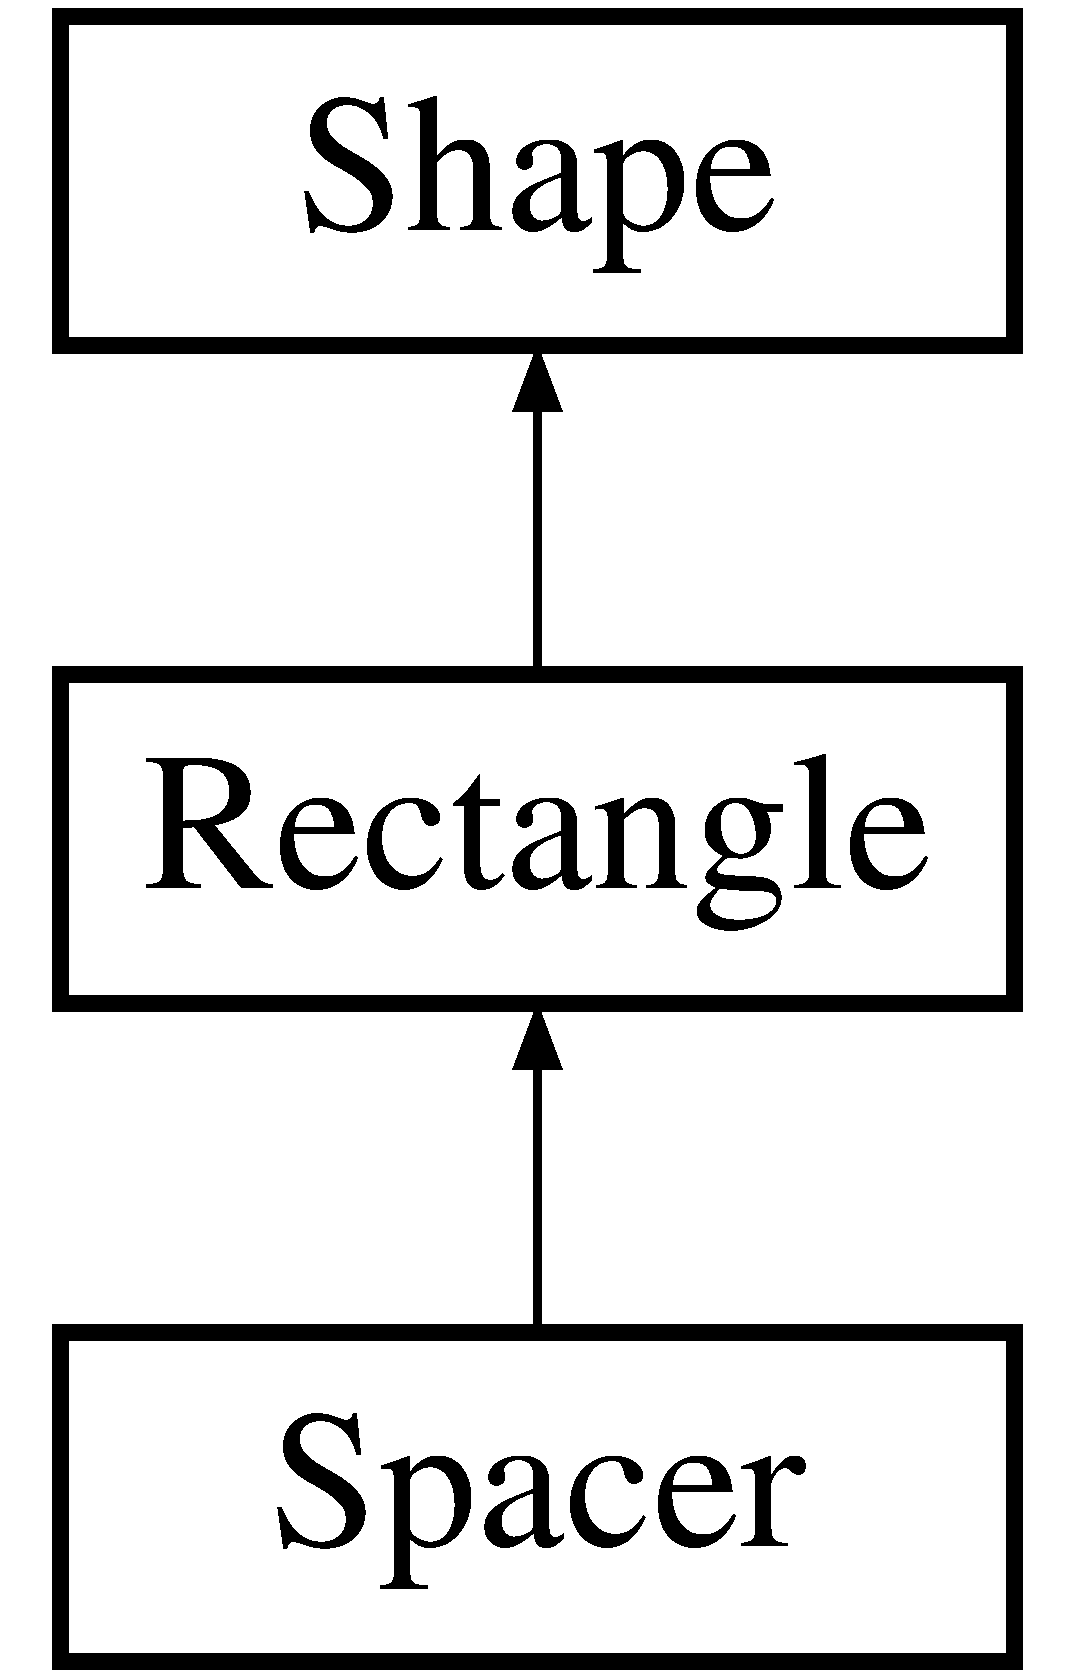
\includegraphics[height=3.000000cm]{class_rectangle}
\end{center}
\end{figure}
\subsection*{Public Member Functions}
\begin{DoxyCompactItemize}
\item 
\hyperlink{class_rectangle_a8a933e0ebd9e80ce91e61ffe87fd577e}{Rectangle} ()
\item 
\hyperlink{class_rectangle_a1dc8d8db9c867aa80616837bd980fd78}{Rectangle} (int \hyperlink{class_shape_a41e403e73d2949f1a6adfba6032c41ec}{x}, int \hyperlink{class_shape_ac757f715cc5b5681f2c691663ac06f0a}{y}, double w, double h)
\item 
\hyperlink{class_rectangle_a361b04e1812db6a4774273d18198f65d}{Rectangle} (double w, double h)
\item 
string \hyperlink{class_rectangle_add9328727ce45f2782971385343a4ea1}{draw} () const 
\begin{DoxyCompactList}\small\item\em generate ps code for shape \end{DoxyCompactList}\item 
string \hyperlink{class_rectangle_ac1cd2c2307b24d001171361f95ea214f}{draw} (int \hyperlink{class_shape_a41e403e73d2949f1a6adfba6032c41ec}{x}, int \hyperlink{class_shape_ac757f715cc5b5681f2c691663ac06f0a}{y}) const 
\begin{DoxyCompactList}\small\item\em generate ps code for shape \end{DoxyCompactList}\end{DoxyCompactItemize}
\subsection*{Protected Attributes}
\begin{DoxyCompactItemize}
\item 
double \hyperlink{class_rectangle_a4a7673968f25a38762439c252b6d877d}{width\+\_\+}
\item 
double \hyperlink{class_rectangle_a3d08f9a12635131e76c4d73a586150d3}{height\+\_\+}
\end{DoxyCompactItemize}


\subsection{Detailed Description}


Definition at line 17 of file rectangle.\+h.



\subsection{Constructor \& Destructor Documentation}
\hypertarget{class_rectangle_a8a933e0ebd9e80ce91e61ffe87fd577e}{}\index{Rectangle@{Rectangle}!Rectangle@{Rectangle}}
\index{Rectangle@{Rectangle}!Rectangle@{Rectangle}}
\subsubsection[{Rectangle()}]{\setlength{\rightskip}{0pt plus 5cm}Rectangle\+::\+Rectangle (
\begin{DoxyParamCaption}
{}
\end{DoxyParamCaption}
)\hspace{0.3cm}{\ttfamily [inline]}}\label{class_rectangle_a8a933e0ebd9e80ce91e61ffe87fd577e}


Definition at line 20 of file rectangle.\+h.

\hypertarget{class_rectangle_a1dc8d8db9c867aa80616837bd980fd78}{}\index{Rectangle@{Rectangle}!Rectangle@{Rectangle}}
\index{Rectangle@{Rectangle}!Rectangle@{Rectangle}}
\subsubsection[{Rectangle(int x, int y, double w, double h)}]{\setlength{\rightskip}{0pt plus 5cm}Rectangle\+::\+Rectangle (
\begin{DoxyParamCaption}
\item[{int}]{x, }
\item[{int}]{y, }
\item[{double}]{w, }
\item[{double}]{h}
\end{DoxyParamCaption}
)\hspace{0.3cm}{\ttfamily [inline]}}\label{class_rectangle_a1dc8d8db9c867aa80616837bd980fd78}


Definition at line 21 of file rectangle.\+h.

\hypertarget{class_rectangle_a361b04e1812db6a4774273d18198f65d}{}\index{Rectangle@{Rectangle}!Rectangle@{Rectangle}}
\index{Rectangle@{Rectangle}!Rectangle@{Rectangle}}
\subsubsection[{Rectangle(double w, double h)}]{\setlength{\rightskip}{0pt plus 5cm}Rectangle\+::\+Rectangle (
\begin{DoxyParamCaption}
\item[{double}]{w, }
\item[{double}]{h}
\end{DoxyParamCaption}
)\hspace{0.3cm}{\ttfamily [inline]}}\label{class_rectangle_a361b04e1812db6a4774273d18198f65d}


Definition at line 22 of file rectangle.\+h.



\subsection{Member Function Documentation}
\hypertarget{class_rectangle_add9328727ce45f2782971385343a4ea1}{}\index{Rectangle@{Rectangle}!draw@{draw}}
\index{draw@{draw}!Rectangle@{Rectangle}}
\subsubsection[{draw() const }]{\setlength{\rightskip}{0pt plus 5cm}string Rectangle\+::draw (
\begin{DoxyParamCaption}
{}
\end{DoxyParamCaption}
) const\hspace{0.3cm}{\ttfamily [virtual]}}\label{class_rectangle_add9328727ce45f2782971385343a4ea1}


generate ps code for shape 

generate ps code for drawing shape at default location \begin{DoxyReturn}{Returns}
string containing ps code for drawing shape at default location 
\end{DoxyReturn}


Reimplemented from \hyperlink{class_shape_a8405e352e8bbbdd173fd89065d63a80b}{Shape}.



Reimplemented in \hyperlink{class_spacer_a9f649a8e182a99584cfd8de8a90423f7}{Spacer}.



Definition at line 11 of file rectangle.\+cpp.

\hypertarget{class_rectangle_ac1cd2c2307b24d001171361f95ea214f}{}\index{Rectangle@{Rectangle}!draw@{draw}}
\index{draw@{draw}!Rectangle@{Rectangle}}
\subsubsection[{draw(int x, int y) const }]{\setlength{\rightskip}{0pt plus 5cm}string Rectangle\+::draw (
\begin{DoxyParamCaption}
\item[{int}]{x, }
\item[{int}]{y}
\end{DoxyParamCaption}
) const\hspace{0.3cm}{\ttfamily [virtual]}}\label{class_rectangle_ac1cd2c2307b24d001171361f95ea214f}


generate ps code for shape 

generate ps code for drawing shape at specified coordinates


\begin{DoxyParams}{Parameters}
{\em x} & x position for center of shape\textquotesingle{}s desired location \\
\hline
{\em y} & y position for center of shape\textquotesingle{}s desired location\\
\hline
\end{DoxyParams}
\begin{DoxyReturn}{Returns}
string containing ps code for drawing shape at specified location 
\end{DoxyReturn}


Reimplemented from \hyperlink{class_shape_af26d06a96ece90a563795ec571451eb1}{Shape}.



Reimplemented in \hyperlink{class_spacer_a7c79d0ca6ccc80a08bdaa839c8e05b2f}{Spacer}.



Definition at line 15 of file rectangle.\+cpp.



\subsection{Member Data Documentation}
\hypertarget{class_rectangle_a3d08f9a12635131e76c4d73a586150d3}{}\index{Rectangle@{Rectangle}!height\+\_\+@{height\+\_\+}}
\index{height\+\_\+@{height\+\_\+}!Rectangle@{Rectangle}}
\subsubsection[{height\+\_\+}]{\setlength{\rightskip}{0pt plus 5cm}double Rectangle\+::height\+\_\+\hspace{0.3cm}{\ttfamily [protected]}}\label{class_rectangle_a3d08f9a12635131e76c4d73a586150d3}
height of rectangle 

Definition at line 35 of file rectangle.\+h.

\hypertarget{class_rectangle_a4a7673968f25a38762439c252b6d877d}{}\index{Rectangle@{Rectangle}!width\+\_\+@{width\+\_\+}}
\index{width\+\_\+@{width\+\_\+}!Rectangle@{Rectangle}}
\subsubsection[{width\+\_\+}]{\setlength{\rightskip}{0pt plus 5cm}double Rectangle\+::width\+\_\+\hspace{0.3cm}{\ttfamily [protected]}}\label{class_rectangle_a4a7673968f25a38762439c252b6d877d}
width of rectangle 

Definition at line 31 of file rectangle.\+h.



The documentation for this class was generated from the following files\+:\begin{DoxyCompactItemize}
\item 
\hyperlink{rectangle_8h}{rectangle.\+h}\item 
\hyperlink{rectangle_8cpp}{rectangle.\+cpp}\end{DoxyCompactItemize}

\hypertarget{class_rotated}{}\section{Rotated Class Reference}
\label{class_rotated}\index{Rotated@{Rotated}}


{\ttfamily \#include $<$rotate.\+h$>$}

Inheritance diagram for Rotated\+:\begin{figure}[H]
\begin{center}
\leavevmode
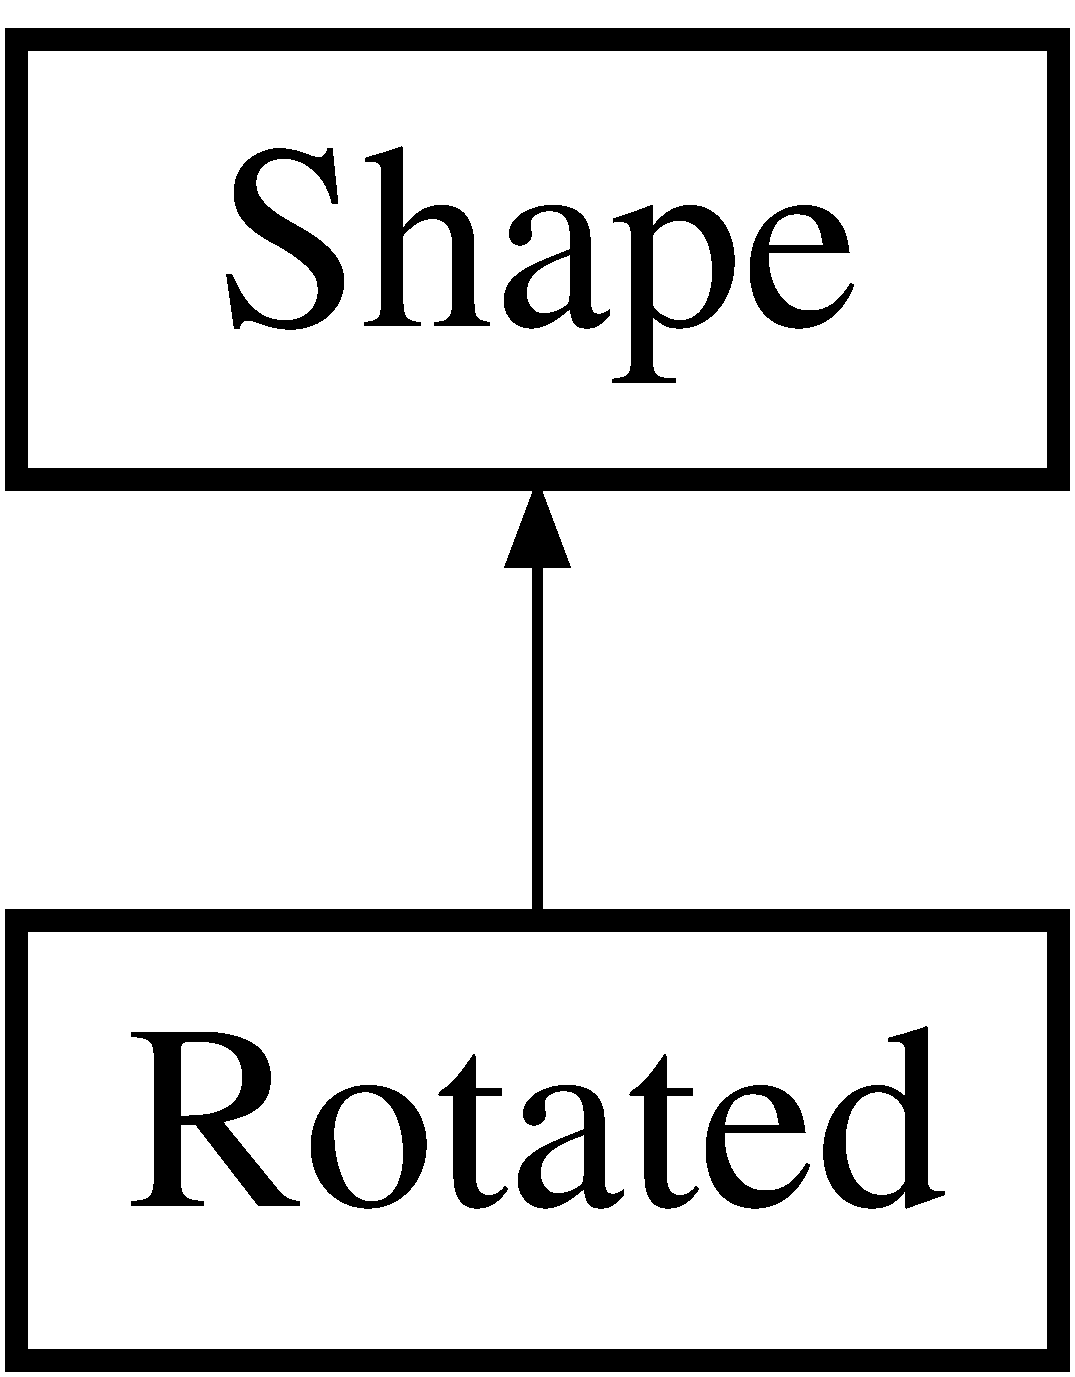
\includegraphics[height=2.000000cm]{class_rotated}
\end{center}
\end{figure}
\subsection*{Public Member Functions}
\begin{DoxyCompactItemize}
\item 
\hyperlink{class_rotated_a0e7bbab1043b5f83912a3963170160aa}{Rotated} ()
\item 
\hyperlink{class_rotated_aee5f88769baea78d5d2fb8f72ac818cf}{Rotated} (\hyperlink{class_shape}{Shape} $\ast$shape, int angle)
\item 
string \hyperlink{class_rotated_ae36addd682056fbd7acef703dc81fafe}{draw} () const 
\begin{DoxyCompactList}\small\item\em generate ps code for shape \end{DoxyCompactList}\item 
string \hyperlink{class_rotated_a1a83cd3f5a9fe6cd99d3eba826f46dd6}{draw} (int \hyperlink{class_shape_a41e403e73d2949f1a6adfba6032c41ec}{x}, int \hyperlink{class_shape_ac757f715cc5b5681f2c691663ac06f0a}{y}) const 
\begin{DoxyCompactList}\small\item\em generate ps code for shape \end{DoxyCompactList}\end{DoxyCompactItemize}
\subsection*{Additional Inherited Members}


\subsection{Detailed Description}


Definition at line 14 of file rotate.\+h.



\subsection{Constructor \& Destructor Documentation}
\hypertarget{class_rotated_a0e7bbab1043b5f83912a3963170160aa}{}\index{Rotated@{Rotated}!Rotated@{Rotated}}
\index{Rotated@{Rotated}!Rotated@{Rotated}}
\subsubsection[{Rotated()}]{\setlength{\rightskip}{0pt plus 5cm}Rotated\+::\+Rotated (
\begin{DoxyParamCaption}
{}
\end{DoxyParamCaption}
)\hspace{0.3cm}{\ttfamily [inline]}}\label{class_rotated_a0e7bbab1043b5f83912a3963170160aa}


Definition at line 17 of file rotate.\+h.

\hypertarget{class_rotated_aee5f88769baea78d5d2fb8f72ac818cf}{}\index{Rotated@{Rotated}!Rotated@{Rotated}}
\index{Rotated@{Rotated}!Rotated@{Rotated}}
\subsubsection[{Rotated(\+Shape $\ast$shape, int angle)}]{\setlength{\rightskip}{0pt plus 5cm}Rotated\+::\+Rotated (
\begin{DoxyParamCaption}
\item[{{\bf Shape} $\ast$}]{shape, }
\item[{int}]{angle}
\end{DoxyParamCaption}
)}\label{class_rotated_aee5f88769baea78d5d2fb8f72ac818cf}


Definition at line 11 of file rotate.\+cpp.



\subsection{Member Function Documentation}
\hypertarget{class_rotated_ae36addd682056fbd7acef703dc81fafe}{}\index{Rotated@{Rotated}!draw@{draw}}
\index{draw@{draw}!Rotated@{Rotated}}
\subsubsection[{draw() const }]{\setlength{\rightskip}{0pt plus 5cm}string Rotated\+::draw (
\begin{DoxyParamCaption}
{}
\end{DoxyParamCaption}
) const\hspace{0.3cm}{\ttfamily [virtual]}}\label{class_rotated_ae36addd682056fbd7acef703dc81fafe}


generate ps code for shape 

generate ps code for drawing shape at default location \begin{DoxyReturn}{Returns}
string containing ps code for drawing shape at default location 
\end{DoxyReturn}


Reimplemented from \hyperlink{class_shape_a8405e352e8bbbdd173fd89065d63a80b}{Shape}.



Definition at line 42 of file rotate.\+cpp.

\hypertarget{class_rotated_a1a83cd3f5a9fe6cd99d3eba826f46dd6}{}\index{Rotated@{Rotated}!draw@{draw}}
\index{draw@{draw}!Rotated@{Rotated}}
\subsubsection[{draw(int x, int y) const }]{\setlength{\rightskip}{0pt plus 5cm}string Rotated\+::draw (
\begin{DoxyParamCaption}
\item[{int}]{x, }
\item[{int}]{y}
\end{DoxyParamCaption}
) const\hspace{0.3cm}{\ttfamily [virtual]}}\label{class_rotated_a1a83cd3f5a9fe6cd99d3eba826f46dd6}


generate ps code for shape 

generate ps code for drawing shape at specified coordinates


\begin{DoxyParams}{Parameters}
{\em x} & x position for center of shape\textquotesingle{}s desired location \\
\hline
{\em y} & y position for center of shape\textquotesingle{}s desired location\\
\hline
\end{DoxyParams}
\begin{DoxyReturn}{Returns}
string containing ps code for drawing shape at specified location 
\end{DoxyReturn}


Reimplemented from \hyperlink{class_shape_af26d06a96ece90a563795ec571451eb1}{Shape}.



Definition at line 46 of file rotate.\+cpp.



The documentation for this class was generated from the following files\+:\begin{DoxyCompactItemize}
\item 
\hyperlink{rotate_8h}{rotate.\+h}\item 
\hyperlink{rotate_8cpp}{rotate.\+cpp}\end{DoxyCompactItemize}

\hypertarget{class_scaled}{}\section{Scaled Class Reference}
\label{class_scaled}\index{Scaled@{Scaled}}


{\ttfamily \#include $<$scaled.\+h$>$}

Inheritance diagram for Scaled\+:\begin{figure}[H]
\begin{center}
\leavevmode
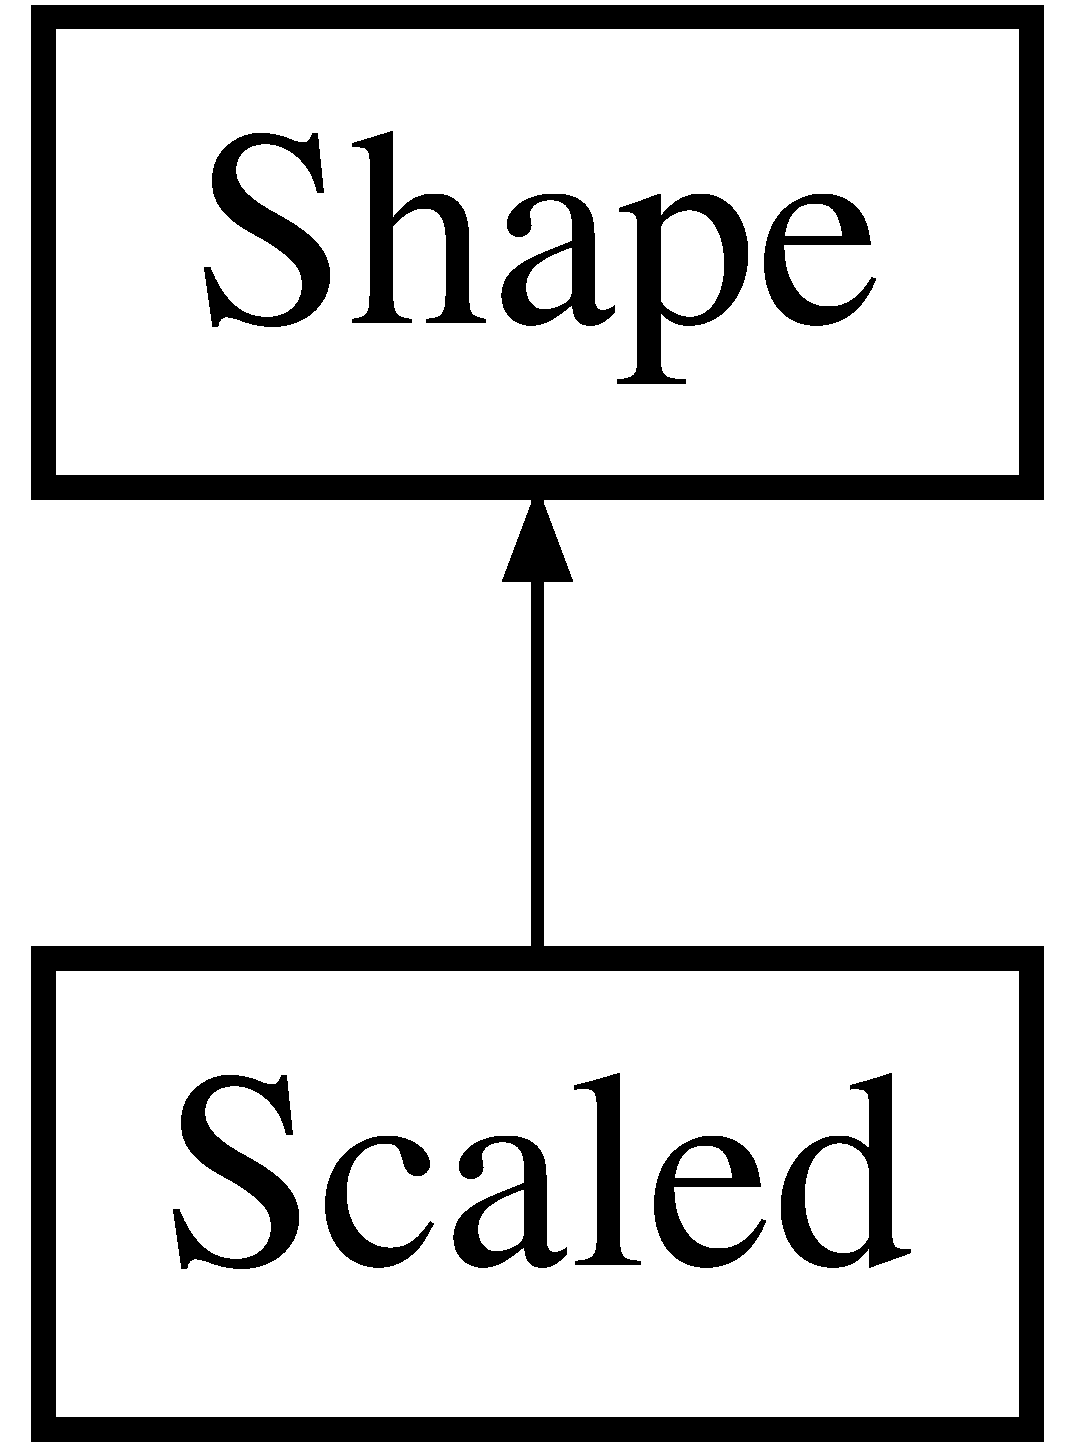
\includegraphics[height=2.000000cm]{class_scaled}
\end{center}
\end{figure}
\subsection*{Public Member Functions}
\begin{DoxyCompactItemize}
\item 
\hyperlink{class_scaled_a77df7ef81f1c3c267cf093c215fe67a8}{Scaled} ()
\item 
\hyperlink{class_scaled_aa0379fdc7d7d44b4735644447386c5c4}{Scaled} (\hyperlink{class_shape}{Shape} $\ast$shape, double sx, double sy)
\item 
string \hyperlink{class_scaled_ad86e14b9c9e880d31b7581134f03e5dc}{draw} () const 
\begin{DoxyCompactList}\small\item\em generate ps code for shape \end{DoxyCompactList}\item 
string \hyperlink{class_scaled_a643010334ff7c4d5cffb98e735a94f8e}{draw} (int \hyperlink{class_shape_a41e403e73d2949f1a6adfba6032c41ec}{x}, int \hyperlink{class_shape_ac757f715cc5b5681f2c691663ac06f0a}{y}) const 
\begin{DoxyCompactList}\small\item\em generate ps code for shape \end{DoxyCompactList}\end{DoxyCompactItemize}
\subsection*{Additional Inherited Members}


\subsection{Detailed Description}


Definition at line 14 of file scaled.\+h.



\subsection{Constructor \& Destructor Documentation}
\hypertarget{class_scaled_a77df7ef81f1c3c267cf093c215fe67a8}{}\index{Scaled@{Scaled}!Scaled@{Scaled}}
\index{Scaled@{Scaled}!Scaled@{Scaled}}
\subsubsection[{Scaled()}]{\setlength{\rightskip}{0pt plus 5cm}Scaled\+::\+Scaled (
\begin{DoxyParamCaption}
{}
\end{DoxyParamCaption}
)\hspace{0.3cm}{\ttfamily [inline]}}\label{class_scaled_a77df7ef81f1c3c267cf093c215fe67a8}


Definition at line 17 of file scaled.\+h.

\hypertarget{class_scaled_aa0379fdc7d7d44b4735644447386c5c4}{}\index{Scaled@{Scaled}!Scaled@{Scaled}}
\index{Scaled@{Scaled}!Scaled@{Scaled}}
\subsubsection[{Scaled(\+Shape $\ast$shape, double sx, double sy)}]{\setlength{\rightskip}{0pt plus 5cm}Scaled\+::\+Scaled (
\begin{DoxyParamCaption}
\item[{{\bf Shape} $\ast$}]{shape, }
\item[{double}]{sx, }
\item[{double}]{sy}
\end{DoxyParamCaption}
)\hspace{0.3cm}{\ttfamily [inline]}}\label{class_scaled_aa0379fdc7d7d44b4735644447386c5c4}


Definition at line 18 of file scaled.\+h.



\subsection{Member Function Documentation}
\hypertarget{class_scaled_ad86e14b9c9e880d31b7581134f03e5dc}{}\index{Scaled@{Scaled}!draw@{draw}}
\index{draw@{draw}!Scaled@{Scaled}}
\subsubsection[{draw() const }]{\setlength{\rightskip}{0pt plus 5cm}string Scaled\+::draw (
\begin{DoxyParamCaption}
{}
\end{DoxyParamCaption}
) const\hspace{0.3cm}{\ttfamily [virtual]}}\label{class_scaled_ad86e14b9c9e880d31b7581134f03e5dc}


generate ps code for shape 

generate ps code for drawing shape at default location \begin{DoxyReturn}{Returns}
string containing ps code for drawing shape at default location 
\end{DoxyReturn}


Reimplemented from \hyperlink{class_shape_a8405e352e8bbbdd173fd89065d63a80b}{Shape}.



Definition at line 11 of file scaled.\+cpp.

\hypertarget{class_scaled_a643010334ff7c4d5cffb98e735a94f8e}{}\index{Scaled@{Scaled}!draw@{draw}}
\index{draw@{draw}!Scaled@{Scaled}}
\subsubsection[{draw(int x, int y) const }]{\setlength{\rightskip}{0pt plus 5cm}string Scaled\+::draw (
\begin{DoxyParamCaption}
\item[{int}]{x, }
\item[{int}]{y}
\end{DoxyParamCaption}
) const\hspace{0.3cm}{\ttfamily [virtual]}}\label{class_scaled_a643010334ff7c4d5cffb98e735a94f8e}


generate ps code for shape 

generate ps code for drawing shape at specified coordinates


\begin{DoxyParams}{Parameters}
{\em x} & x position for center of shape\textquotesingle{}s desired location \\
\hline
{\em y} & y position for center of shape\textquotesingle{}s desired location\\
\hline
\end{DoxyParams}
\begin{DoxyReturn}{Returns}
string containing ps code for drawing shape at specified location 
\end{DoxyReturn}


Reimplemented from \hyperlink{class_shape_af26d06a96ece90a563795ec571451eb1}{Shape}.



Definition at line 15 of file scaled.\+cpp.



The documentation for this class was generated from the following files\+:\begin{DoxyCompactItemize}
\item 
\hyperlink{scaled_8h}{scaled.\+h}\item 
\hyperlink{scaled_8cpp}{scaled.\+cpp}\end{DoxyCompactItemize}

\hypertarget{class_shape}{}\section{Shape Class Reference}
\label{class_shape}\index{Shape@{Shape}}


{\ttfamily \#include $<$shape.\+h$>$}

Inheritance diagram for Shape\+:\begin{figure}[H]
\begin{center}
\leavevmode
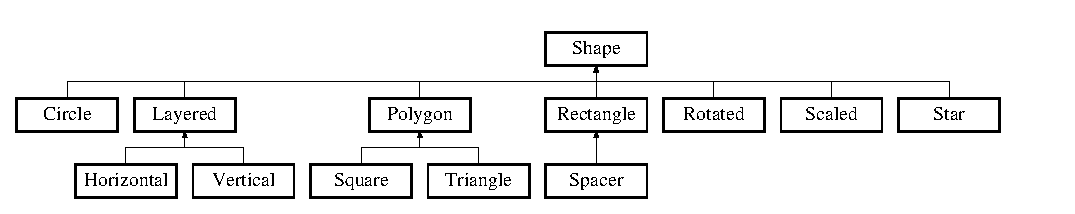
\includegraphics[height=2.424242cm]{class_shape}
\end{center}
\end{figure}
\subsection*{Public Member Functions}
\begin{DoxyCompactItemize}
\item 
\hyperlink{class_shape_aaa8d87171e65e0d8ba3c5459978992a7}{Shape} ()
\item 
\hyperlink{class_shape_a06ed78198a1e3f0940d5e72006c3a074}{Shape} (int \hyperlink{class_shape_a41e403e73d2949f1a6adfba6032c41ec}{x}, int \hyperlink{class_shape_ac757f715cc5b5681f2c691663ac06f0a}{y}, double \hyperlink{class_shape_ab00e62f9f7cd0be450ac29437b80ce13}{width}, double \hyperlink{class_shape_a11686d7b1511fc6707f4dd7b74c65111}{height})
\item 
\hyperlink{class_shape_af3e449cf02a5f99a7c0d11873756b81f}{Shape} (double \hyperlink{class_shape_ab00e62f9f7cd0be450ac29437b80ce13}{width}, double \hyperlink{class_shape_a11686d7b1511fc6707f4dd7b74c65111}{height})
\item 
virtual \hyperlink{class_shape_ac3b9fc48965274893f25b18aa14ba665}{$\sim$\+Shape} ()
\item 
virtual string \hyperlink{class_shape_a8405e352e8bbbdd173fd89065d63a80b}{draw} () const 
\begin{DoxyCompactList}\small\item\em generate ps code for shape \end{DoxyCompactList}\item 
virtual string \hyperlink{class_shape_af26d06a96ece90a563795ec571451eb1}{draw} (int \hyperlink{class_shape_a41e403e73d2949f1a6adfba6032c41ec}{x}, int \hyperlink{class_shape_ac757f715cc5b5681f2c691663ac06f0a}{y}) const 
\begin{DoxyCompactList}\small\item\em generate ps code for shape \end{DoxyCompactList}\item 
virtual void \hyperlink{class_shape_a9d6b2e7274a0e1708d5ec93613b53ef2}{place} (int \hyperlink{class_shape_a41e403e73d2949f1a6adfba6032c41ec}{x}, int \hyperlink{class_shape_ac757f715cc5b5681f2c691663ac06f0a}{y})
\begin{DoxyCompactList}\small\item\em change shape position \end{DoxyCompactList}\item 
string \hyperlink{class_shape_a8b66fe7fe3e0e3ad883eb5d487d8d442}{bounds} ()
\begin{DoxyCompactList}\small\item\em shape boundary \end{DoxyCompactList}\item 
double \hyperlink{class_shape_ab00e62f9f7cd0be450ac29437b80ce13}{width} ()
\begin{DoxyCompactList}\small\item\em get boundary width \end{DoxyCompactList}\item 
double \hyperlink{class_shape_a11686d7b1511fc6707f4dd7b74c65111}{height} ()
\begin{DoxyCompactList}\small\item\em get boundary box height \end{DoxyCompactList}\item 
int \hyperlink{class_shape_a41e403e73d2949f1a6adfba6032c41ec}{x} ()
\begin{DoxyCompactList}\small\item\em get x \end{DoxyCompactList}\item 
void \hyperlink{class_shape_adc67c1bfb923ed3d7e0cfe4a0cd34f29}{x} (int x)
\begin{DoxyCompactList}\small\item\em set x \end{DoxyCompactList}\item 
int \hyperlink{class_shape_ac757f715cc5b5681f2c691663ac06f0a}{y} ()
\begin{DoxyCompactList}\small\item\em get y \end{DoxyCompactList}\item 
void \hyperlink{class_shape_ae3245e558aad6f812b108632aed6745f}{y} (int y)
\begin{DoxyCompactList}\small\item\em sets y \end{DoxyCompactList}\item 
string \hyperlink{class_shape_ac3ac785096912e7b1b3c0ac603714482}{operator()} ()
\begin{DoxyCompactList}\small\item\em draw shape at position \end{DoxyCompactList}\item 
string \hyperlink{class_shape_ab188d62cc440aeaab8407b32caaa8823}{operator()} (int \hyperlink{class_shape_a41e403e73d2949f1a6adfba6032c41ec}{x}, int \hyperlink{class_shape_ac757f715cc5b5681f2c691663ac06f0a}{y})
\begin{DoxyCompactList}\small\item\em draw shape at position \end{DoxyCompactList}\item 
virtual int \hyperlink{class_shape_ac152ef6b8150122e1e279e3ac2d9b627}{num\+Of\+Sides} ()
\begin{DoxyCompactList}\small\item\em returns number of sides \end{DoxyCompactList}\item 
virtual double \hyperlink{class_shape_a116897479aa63aeea80648b7ac9e114a}{side\+Length} ()
\begin{DoxyCompactList}\small\item\em returns side length \end{DoxyCompactList}\item 
virtual double \hyperlink{class_shape_a8193b252afa84bbf0b173160d2b3302d}{radius} ()
\begin{DoxyCompactList}\small\item\em returns radius \end{DoxyCompactList}\end{DoxyCompactItemize}
\subsection*{Protected Attributes}
\begin{DoxyCompactItemize}
\item 
int \hyperlink{class_shape_ac9f855989a11f0baf8c6a0a494270a2c}{x\+\_\+}
\item 
int \hyperlink{class_shape_ae85309f9b9f6ecb7713ebe1d6891126b}{y\+\_\+}
\item 
double \hyperlink{class_shape_a8d608b3645ea020c08eaabfd112bd5d4}{bounds\+Width\+\_\+}
\item 
double \hyperlink{class_shape_a99e0e92930da8380eedae20255347b50}{bounds\+Height\+\_\+}
\end{DoxyCompactItemize}


\subsection{Detailed Description}


Definition at line 28 of file shape.\+h.



\subsection{Constructor \& Destructor Documentation}
\hypertarget{class_shape_aaa8d87171e65e0d8ba3c5459978992a7}{}\index{Shape@{Shape}!Shape@{Shape}}
\index{Shape@{Shape}!Shape@{Shape}}
\subsubsection[{Shape()}]{\setlength{\rightskip}{0pt plus 5cm}Shape\+::\+Shape (
\begin{DoxyParamCaption}
{}
\end{DoxyParamCaption}
)\hspace{0.3cm}{\ttfamily [inline]}}\label{class_shape_aaa8d87171e65e0d8ba3c5459978992a7}


Definition at line 32 of file shape.\+h.

\hypertarget{class_shape_a06ed78198a1e3f0940d5e72006c3a074}{}\index{Shape@{Shape}!Shape@{Shape}}
\index{Shape@{Shape}!Shape@{Shape}}
\subsubsection[{Shape(int x, int y, double width, double height)}]{\setlength{\rightskip}{0pt plus 5cm}Shape\+::\+Shape (
\begin{DoxyParamCaption}
\item[{int}]{x, }
\item[{int}]{y, }
\item[{double}]{width, }
\item[{double}]{height}
\end{DoxyParamCaption}
)\hspace{0.3cm}{\ttfamily [inline]}}\label{class_shape_a06ed78198a1e3f0940d5e72006c3a074}


Definition at line 33 of file shape.\+h.

\hypertarget{class_shape_af3e449cf02a5f99a7c0d11873756b81f}{}\index{Shape@{Shape}!Shape@{Shape}}
\index{Shape@{Shape}!Shape@{Shape}}
\subsubsection[{Shape(double width, double height)}]{\setlength{\rightskip}{0pt plus 5cm}Shape\+::\+Shape (
\begin{DoxyParamCaption}
\item[{double}]{width, }
\item[{double}]{height}
\end{DoxyParamCaption}
)\hspace{0.3cm}{\ttfamily [inline]}}\label{class_shape_af3e449cf02a5f99a7c0d11873756b81f}


Definition at line 34 of file shape.\+h.

\hypertarget{class_shape_ac3b9fc48965274893f25b18aa14ba665}{}\index{Shape@{Shape}!````~Shape@{$\sim$\+Shape}}
\index{````~Shape@{$\sim$\+Shape}!Shape@{Shape}}
\subsubsection[{$\sim$\+Shape()}]{\setlength{\rightskip}{0pt plus 5cm}virtual Shape\+::$\sim$\+Shape (
\begin{DoxyParamCaption}
{}
\end{DoxyParamCaption}
)\hspace{0.3cm}{\ttfamily [inline]}, {\ttfamily [virtual]}}\label{class_shape_ac3b9fc48965274893f25b18aa14ba665}


Definition at line 36 of file shape.\+h.



\subsection{Member Function Documentation}
\hypertarget{class_shape_a8b66fe7fe3e0e3ad883eb5d487d8d442}{}\index{Shape@{Shape}!bounds@{bounds}}
\index{bounds@{bounds}!Shape@{Shape}}
\subsubsection[{bounds()}]{\setlength{\rightskip}{0pt plus 5cm}string Shape\+::bounds (
\begin{DoxyParamCaption}
{}
\end{DoxyParamCaption}
)}\label{class_shape_a8b66fe7fe3e0e3ad883eb5d487d8d442}


shape boundary 

generates string with the values of boundary box witdth and height \begin{DoxyReturn}{Returns}
string with boundary 
\end{DoxyReturn}


Definition at line 50 of file shape.\+cpp.

\hypertarget{class_shape_a8405e352e8bbbdd173fd89065d63a80b}{}\index{Shape@{Shape}!draw@{draw}}
\index{draw@{draw}!Shape@{Shape}}
\subsubsection[{draw() const }]{\setlength{\rightskip}{0pt plus 5cm}string Shape\+::draw (
\begin{DoxyParamCaption}
{}
\end{DoxyParamCaption}
) const\hspace{0.3cm}{\ttfamily [virtual]}}\label{class_shape_a8405e352e8bbbdd173fd89065d63a80b}


generate ps code for shape 

generate ps code for drawing shape at default location \begin{DoxyReturn}{Returns}
string containing ps code for drawing shape at default location 
\end{DoxyReturn}


Reimplemented in \hyperlink{class_vertical_a778fd2aa48afcf255b75413e29613ebb}{Vertical}, \hyperlink{class_horizontal_a79e26b6d0db2a2b7e4f25a3f0f67e7a2}{Horizontal}, \hyperlink{class_polygon_a732b40203a5cc2baadd90446c3ec8213}{Polygon}, \hyperlink{class_scaled_ad86e14b9c9e880d31b7581134f03e5dc}{Scaled}, \hyperlink{class_layered_a968cd141e61eb039b997352a318dcae0}{Layered}, \hyperlink{class_rectangle_add9328727ce45f2782971385343a4ea1}{Rectangle}, \hyperlink{class_circle_a3fcc66abd3f30a3c19e3bb63452fc2ed}{Circle}, \hyperlink{class_spacer_a9f649a8e182a99584cfd8de8a90423f7}{Spacer}, \hyperlink{class_star_ae0187621a33e5b704f92c77089250316}{Star}, and \hyperlink{class_rotated_ae36addd682056fbd7acef703dc81fafe}{Rotated}.



Definition at line 16 of file shape.\+cpp.

\hypertarget{class_shape_af26d06a96ece90a563795ec571451eb1}{}\index{Shape@{Shape}!draw@{draw}}
\index{draw@{draw}!Shape@{Shape}}
\subsubsection[{draw(int x, int y) const }]{\setlength{\rightskip}{0pt plus 5cm}string Shape\+::draw (
\begin{DoxyParamCaption}
\item[{int}]{x, }
\item[{int}]{y}
\end{DoxyParamCaption}
) const\hspace{0.3cm}{\ttfamily [virtual]}}\label{class_shape_af26d06a96ece90a563795ec571451eb1}


generate ps code for shape 

generate ps code for drawing shape at specified coordinates


\begin{DoxyParams}{Parameters}
{\em x} & x position for center of shape\textquotesingle{}s desired location \\
\hline
{\em y} & y position for center of shape\textquotesingle{}s desired location\\
\hline
\end{DoxyParams}
\begin{DoxyReturn}{Returns}
string containing ps code for drawing shape at specified location 
\end{DoxyReturn}


Reimplemented in \hyperlink{class_vertical_a9be329f986230ccaa35ec7f63553d658}{Vertical}, \hyperlink{class_horizontal_aea100857d1a9a269b66060b8bd32ced1}{Horizontal}, \hyperlink{class_polygon_af0f4e693010935528bb3e99bca2cc433}{Polygon}, \hyperlink{class_scaled_a643010334ff7c4d5cffb98e735a94f8e}{Scaled}, \hyperlink{class_layered_a6eb564ff0646b26fdd4175856b1a0815}{Layered}, \hyperlink{class_rectangle_ac1cd2c2307b24d001171361f95ea214f}{Rectangle}, \hyperlink{class_circle_a18f2b8aaa80fb870c3aea1798f32678b}{Circle}, \hyperlink{class_spacer_a7c79d0ca6ccc80a08bdaa839c8e05b2f}{Spacer}, \hyperlink{class_star_abb1a219aa29c63205f1e23a056aae521}{Star}, and \hyperlink{class_rotated_a1a83cd3f5a9fe6cd99d3eba826f46dd6}{Rotated}.



Definition at line 29 of file shape.\+cpp.

\hypertarget{class_shape_a11686d7b1511fc6707f4dd7b74c65111}{}\index{Shape@{Shape}!height@{height}}
\index{height@{height}!Shape@{Shape}}
\subsubsection[{height()}]{\setlength{\rightskip}{0pt plus 5cm}double Shape\+::height (
\begin{DoxyParamCaption}
{}
\end{DoxyParamCaption}
)}\label{class_shape_a11686d7b1511fc6707f4dd7b74c65111}


get boundary box height 

get the double containing the height of the shape\textquotesingle{}s boundary box \begin{DoxyReturn}{Returns}
double boundary height 
\end{DoxyReturn}


Definition at line 70 of file shape.\+cpp.

\hypertarget{class_shape_ac152ef6b8150122e1e279e3ac2d9b627}{}\index{Shape@{Shape}!num\+Of\+Sides@{num\+Of\+Sides}}
\index{num\+Of\+Sides@{num\+Of\+Sides}!Shape@{Shape}}
\subsubsection[{num\+Of\+Sides()}]{\setlength{\rightskip}{0pt plus 5cm}int Shape\+::num\+Of\+Sides (
\begin{DoxyParamCaption}
{}
\end{DoxyParamCaption}
)\hspace{0.3cm}{\ttfamily [virtual]}}\label{class_shape_ac152ef6b8150122e1e279e3ac2d9b627}


returns number of sides 

returns number of sides of a shape, only defined for \hyperlink{class_polygon}{Polygon} \begin{DoxyReturn}{Returns}
if \hyperlink{class_polygon}{Polygon}, returns number of sides. Otherwise returns 0. 
\end{DoxyReturn}


Reimplemented in \hyperlink{class_polygon_a3c57ca9893bf151501123b8b1787acf6}{Polygon}.



Definition at line 139 of file shape.\+cpp.

\hypertarget{class_shape_ac3ac785096912e7b1b3c0ac603714482}{}\index{Shape@{Shape}!operator()@{operator()}}
\index{operator()@{operator()}!Shape@{Shape}}
\subsubsection[{operator()()}]{\setlength{\rightskip}{0pt plus 5cm}string Shape\+::operator() (
\begin{DoxyParamCaption}
{}
\end{DoxyParamCaption}
)}\label{class_shape_ac3ac785096912e7b1b3c0ac603714482}


draw shape at position 

generates ps code for drawing a shape at the shape\textquotesingle{}s set location \begin{DoxyReturn}{Returns}
string containing ps code 
\end{DoxyReturn}


Definition at line 117 of file shape.\+cpp.

\hypertarget{class_shape_ab188d62cc440aeaab8407b32caaa8823}{}\index{Shape@{Shape}!operator()@{operator()}}
\index{operator()@{operator()}!Shape@{Shape}}
\subsubsection[{operator()(int x, int y)}]{\setlength{\rightskip}{0pt plus 5cm}string Shape\+::operator() (
\begin{DoxyParamCaption}
\item[{int}]{x, }
\item[{int}]{y}
\end{DoxyParamCaption}
)}\label{class_shape_ab188d62cc440aeaab8407b32caaa8823}


draw shape at position 

generates ps code for drawing shape at specified location


\begin{DoxyParams}{Parameters}
{\em x} & x position of center of shape \\
\hline
{\em y} & y position of center of shape\\
\hline
\end{DoxyParams}
\begin{DoxyReturn}{Returns}
string containing ps code 
\end{DoxyReturn}


Definition at line 130 of file shape.\+cpp.

\hypertarget{class_shape_a9d6b2e7274a0e1708d5ec93613b53ef2}{}\index{Shape@{Shape}!place@{place}}
\index{place@{place}!Shape@{Shape}}
\subsubsection[{place(int x, int y)}]{\setlength{\rightskip}{0pt plus 5cm}void Shape\+::place (
\begin{DoxyParamCaption}
\item[{int}]{x, }
\item[{int}]{y}
\end{DoxyParamCaption}
)\hspace{0.3cm}{\ttfamily [virtual]}}\label{class_shape_a9d6b2e7274a0e1708d5ec93613b53ef2}


change shape position 

change shape position to passed coordinates


\begin{DoxyParams}{Parameters}
{\em x} & x coordinate of new position \\
\hline
{\em y} & y coordinate of new position \\
\hline
\end{DoxyParams}


Definition at line 40 of file shape.\+cpp.

\hypertarget{class_shape_a8193b252afa84bbf0b173160d2b3302d}{}\index{Shape@{Shape}!radius@{radius}}
\index{radius@{radius}!Shape@{Shape}}
\subsubsection[{radius()}]{\setlength{\rightskip}{0pt plus 5cm}double Shape\+::radius (
\begin{DoxyParamCaption}
{}
\end{DoxyParamCaption}
)\hspace{0.3cm}{\ttfamily [virtual]}}\label{class_shape_a8193b252afa84bbf0b173160d2b3302d}


returns radius 

returns the radius of a shape, only defined for \hyperlink{class_polygon}{Polygon} and \hyperlink{class_circle}{Circle} \begin{DoxyReturn}{Returns}
if \hyperlink{class_polygon}{Polygon} or \hyperlink{class_circle}{Circle}, returns the radius. Otherwise returns 0. 
\end{DoxyReturn}


Reimplemented in \hyperlink{class_polygon_af1af4ce31b24eb31b4300e932f2578c2}{Polygon}, and \hyperlink{class_circle_addf06b37dda7589ade30e7ea21fe17be}{Circle}.



Definition at line 157 of file shape.\+cpp.

\hypertarget{class_shape_a116897479aa63aeea80648b7ac9e114a}{}\index{Shape@{Shape}!side\+Length@{side\+Length}}
\index{side\+Length@{side\+Length}!Shape@{Shape}}
\subsubsection[{side\+Length()}]{\setlength{\rightskip}{0pt plus 5cm}double Shape\+::side\+Length (
\begin{DoxyParamCaption}
{}
\end{DoxyParamCaption}
)\hspace{0.3cm}{\ttfamily [virtual]}}\label{class_shape_a116897479aa63aeea80648b7ac9e114a}


returns side length 

returns length of a side of a shape, only defined for \hyperlink{class_polygon}{Polygon} \begin{DoxyReturn}{Returns}
if \hyperlink{class_polygon}{Polygon}, returns length of a side. Otherwise returns 0. 
\end{DoxyReturn}


Reimplemented in \hyperlink{class_polygon_ab03b3c38a9f26b2c0d46294dd77f4318}{Polygon}.



Definition at line 148 of file shape.\+cpp.

\hypertarget{class_shape_ab00e62f9f7cd0be450ac29437b80ce13}{}\index{Shape@{Shape}!width@{width}}
\index{width@{width}!Shape@{Shape}}
\subsubsection[{width()}]{\setlength{\rightskip}{0pt plus 5cm}double Shape\+::width (
\begin{DoxyParamCaption}
{}
\end{DoxyParamCaption}
)}\label{class_shape_ab00e62f9f7cd0be450ac29437b80ce13}


get boundary width 

get the double containing the width of the shape\textquotesingle{}s boundary box \begin{DoxyReturn}{Returns}
double boundary width 
\end{DoxyReturn}


Definition at line 61 of file shape.\+cpp.

\hypertarget{class_shape_a41e403e73d2949f1a6adfba6032c41ec}{}\index{Shape@{Shape}!x@{x}}
\index{x@{x}!Shape@{Shape}}
\subsubsection[{x()}]{\setlength{\rightskip}{0pt plus 5cm}int Shape\+::x (
\begin{DoxyParamCaption}
{}
\end{DoxyParamCaption}
)}\label{class_shape_a41e403e73d2949f1a6adfba6032c41ec}


get x 

gets x value of center of shape \begin{DoxyReturn}{Returns}
returns x 
\end{DoxyReturn}


Definition at line 79 of file shape.\+cpp.

\hypertarget{class_shape_adc67c1bfb923ed3d7e0cfe4a0cd34f29}{}\index{Shape@{Shape}!x@{x}}
\index{x@{x}!Shape@{Shape}}
\subsubsection[{x(int x)}]{\setlength{\rightskip}{0pt plus 5cm}void Shape\+::x (
\begin{DoxyParamCaption}
\item[{int}]{x}
\end{DoxyParamCaption}
)}\label{class_shape_adc67c1bfb923ed3d7e0cfe4a0cd34f29}


set x 

sets x value of center of shape


\begin{DoxyParams}{Parameters}
{\em x} & new x value \\
\hline
\end{DoxyParams}


Definition at line 89 of file shape.\+cpp.

\hypertarget{class_shape_ac757f715cc5b5681f2c691663ac06f0a}{}\index{Shape@{Shape}!y@{y}}
\index{y@{y}!Shape@{Shape}}
\subsubsection[{y()}]{\setlength{\rightskip}{0pt plus 5cm}int Shape\+::y (
\begin{DoxyParamCaption}
{}
\end{DoxyParamCaption}
)}\label{class_shape_ac757f715cc5b5681f2c691663ac06f0a}


get y 

gets y value of center of shape \begin{DoxyReturn}{Returns}
returns y 
\end{DoxyReturn}


Definition at line 98 of file shape.\+cpp.

\hypertarget{class_shape_ae3245e558aad6f812b108632aed6745f}{}\index{Shape@{Shape}!y@{y}}
\index{y@{y}!Shape@{Shape}}
\subsubsection[{y(int y)}]{\setlength{\rightskip}{0pt plus 5cm}void Shape\+::y (
\begin{DoxyParamCaption}
\item[{int}]{y}
\end{DoxyParamCaption}
)}\label{class_shape_ae3245e558aad6f812b108632aed6745f}


sets y 

sets y value of center of shape


\begin{DoxyParams}{Parameters}
{\em y} & new y value \\
\hline
\end{DoxyParams}


Definition at line 108 of file shape.\+cpp.



\subsection{Member Data Documentation}
\hypertarget{class_shape_a99e0e92930da8380eedae20255347b50}{}\index{Shape@{Shape}!bounds\+Height\+\_\+@{bounds\+Height\+\_\+}}
\index{bounds\+Height\+\_\+@{bounds\+Height\+\_\+}!Shape@{Shape}}
\subsubsection[{bounds\+Height\+\_\+}]{\setlength{\rightskip}{0pt plus 5cm}double Shape\+::bounds\+Height\+\_\+\hspace{0.3cm}{\ttfamily [protected]}}\label{class_shape_a99e0e92930da8380eedae20255347b50}
height of boundary box 

Definition at line 76 of file shape.\+h.

\hypertarget{class_shape_a8d608b3645ea020c08eaabfd112bd5d4}{}\index{Shape@{Shape}!bounds\+Width\+\_\+@{bounds\+Width\+\_\+}}
\index{bounds\+Width\+\_\+@{bounds\+Width\+\_\+}!Shape@{Shape}}
\subsubsection[{bounds\+Width\+\_\+}]{\setlength{\rightskip}{0pt plus 5cm}double Shape\+::bounds\+Width\+\_\+\hspace{0.3cm}{\ttfamily [protected]}}\label{class_shape_a8d608b3645ea020c08eaabfd112bd5d4}
width of boundary box 

Definition at line 71 of file shape.\+h.

\hypertarget{class_shape_ac9f855989a11f0baf8c6a0a494270a2c}{}\index{Shape@{Shape}!x\+\_\+@{x\+\_\+}}
\index{x\+\_\+@{x\+\_\+}!Shape@{Shape}}
\subsubsection[{x\+\_\+}]{\setlength{\rightskip}{0pt plus 5cm}int Shape\+::x\+\_\+\hspace{0.3cm}{\ttfamily [protected]}}\label{class_shape_ac9f855989a11f0baf8c6a0a494270a2c}
x coordinate of shape position 

Definition at line 61 of file shape.\+h.

\hypertarget{class_shape_ae85309f9b9f6ecb7713ebe1d6891126b}{}\index{Shape@{Shape}!y\+\_\+@{y\+\_\+}}
\index{y\+\_\+@{y\+\_\+}!Shape@{Shape}}
\subsubsection[{y\+\_\+}]{\setlength{\rightskip}{0pt plus 5cm}int Shape\+::y\+\_\+\hspace{0.3cm}{\ttfamily [protected]}}\label{class_shape_ae85309f9b9f6ecb7713ebe1d6891126b}
y coordinate of shape position 

Definition at line 66 of file shape.\+h.



The documentation for this class was generated from the following files\+:\begin{DoxyCompactItemize}
\item 
\hyperlink{shape_8h}{shape.\+h}\item 
\hyperlink{shape_8cpp}{shape.\+cpp}\end{DoxyCompactItemize}

\hypertarget{class_spacer}{}\section{Spacer Class Reference}
\label{class_spacer}\index{Spacer@{Spacer}}


{\ttfamily \#include $<$spacer.\+h$>$}

Inheritance diagram for Spacer\+:\begin{figure}[H]
\begin{center}
\leavevmode
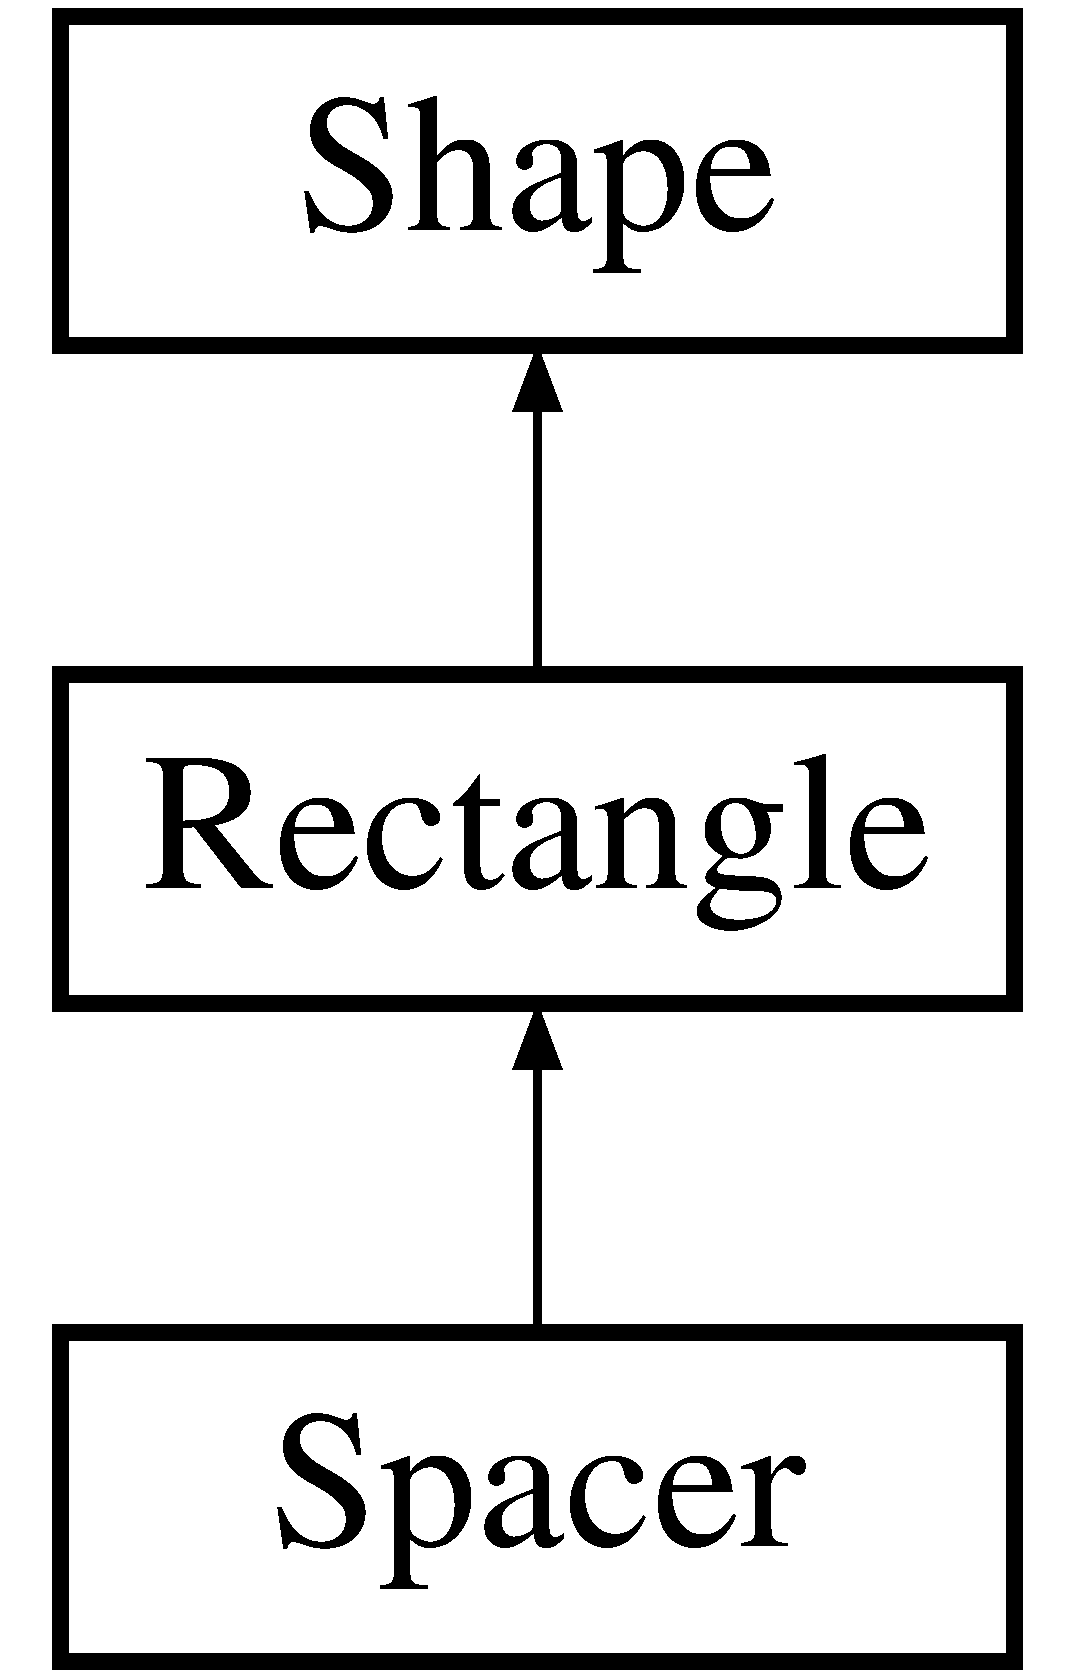
\includegraphics[height=3.000000cm]{class_spacer}
\end{center}
\end{figure}
\subsection*{Public Member Functions}
\begin{DoxyCompactItemize}
\item 
\hyperlink{class_spacer_a633ff31f694cbefad661ba67c0a4b11b}{Spacer} ()
\item 
\hyperlink{class_spacer_a358ef503c38bd3b6b370de2e8eb1b603}{Spacer} (int \hyperlink{class_shape_a41e403e73d2949f1a6adfba6032c41ec}{x}, int \hyperlink{class_shape_ac757f715cc5b5681f2c691663ac06f0a}{y}, double w, double h)
\item 
\hyperlink{class_spacer_a33874d4aa3de2963b2672e3b50a41eb2}{Spacer} (double w, double h)
\item 
string \hyperlink{class_spacer_a9f649a8e182a99584cfd8de8a90423f7}{draw} () const 
\begin{DoxyCompactList}\small\item\em generate ps code for shape \end{DoxyCompactList}\item 
string \hyperlink{class_spacer_a7c79d0ca6ccc80a08bdaa839c8e05b2f}{draw} (int \hyperlink{class_shape_a41e403e73d2949f1a6adfba6032c41ec}{x}, int \hyperlink{class_shape_ac757f715cc5b5681f2c691663ac06f0a}{y}) const 
\begin{DoxyCompactList}\small\item\em generate ps code for shape \end{DoxyCompactList}\end{DoxyCompactItemize}
\subsection*{Additional Inherited Members}


\subsection{Detailed Description}


Definition at line 14 of file spacer.\+h.



\subsection{Constructor \& Destructor Documentation}
\hypertarget{class_spacer_a633ff31f694cbefad661ba67c0a4b11b}{}\index{Spacer@{Spacer}!Spacer@{Spacer}}
\index{Spacer@{Spacer}!Spacer@{Spacer}}
\subsubsection[{Spacer()}]{\setlength{\rightskip}{0pt plus 5cm}Spacer\+::\+Spacer (
\begin{DoxyParamCaption}
{}
\end{DoxyParamCaption}
)\hspace{0.3cm}{\ttfamily [inline]}}\label{class_spacer_a633ff31f694cbefad661ba67c0a4b11b}


Definition at line 17 of file spacer.\+h.

\hypertarget{class_spacer_a358ef503c38bd3b6b370de2e8eb1b603}{}\index{Spacer@{Spacer}!Spacer@{Spacer}}
\index{Spacer@{Spacer}!Spacer@{Spacer}}
\subsubsection[{Spacer(int x, int y, double w, double h)}]{\setlength{\rightskip}{0pt plus 5cm}Spacer\+::\+Spacer (
\begin{DoxyParamCaption}
\item[{int}]{x, }
\item[{int}]{y, }
\item[{double}]{w, }
\item[{double}]{h}
\end{DoxyParamCaption}
)\hspace{0.3cm}{\ttfamily [inline]}}\label{class_spacer_a358ef503c38bd3b6b370de2e8eb1b603}


Definition at line 18 of file spacer.\+h.

\hypertarget{class_spacer_a33874d4aa3de2963b2672e3b50a41eb2}{}\index{Spacer@{Spacer}!Spacer@{Spacer}}
\index{Spacer@{Spacer}!Spacer@{Spacer}}
\subsubsection[{Spacer(double w, double h)}]{\setlength{\rightskip}{0pt plus 5cm}Spacer\+::\+Spacer (
\begin{DoxyParamCaption}
\item[{double}]{w, }
\item[{double}]{h}
\end{DoxyParamCaption}
)\hspace{0.3cm}{\ttfamily [inline]}}\label{class_spacer_a33874d4aa3de2963b2672e3b50a41eb2}


Definition at line 19 of file spacer.\+h.



\subsection{Member Function Documentation}
\hypertarget{class_spacer_a9f649a8e182a99584cfd8de8a90423f7}{}\index{Spacer@{Spacer}!draw@{draw}}
\index{draw@{draw}!Spacer@{Spacer}}
\subsubsection[{draw() const }]{\setlength{\rightskip}{0pt plus 5cm}string Spacer\+::draw (
\begin{DoxyParamCaption}
{}
\end{DoxyParamCaption}
) const\hspace{0.3cm}{\ttfamily [virtual]}}\label{class_spacer_a9f649a8e182a99584cfd8de8a90423f7}


generate ps code for shape 

generate ps code for drawing shape at default location \begin{DoxyReturn}{Returns}
string containing ps code for drawing shape at default location 
\end{DoxyReturn}


Reimplemented from \hyperlink{class_rectangle_add9328727ce45f2782971385343a4ea1}{Rectangle}.



Definition at line 11 of file spacer.\+cpp.

\hypertarget{class_spacer_a7c79d0ca6ccc80a08bdaa839c8e05b2f}{}\index{Spacer@{Spacer}!draw@{draw}}
\index{draw@{draw}!Spacer@{Spacer}}
\subsubsection[{draw(int x, int y) const }]{\setlength{\rightskip}{0pt plus 5cm}string Spacer\+::draw (
\begin{DoxyParamCaption}
\item[{int}]{x, }
\item[{int}]{y}
\end{DoxyParamCaption}
) const\hspace{0.3cm}{\ttfamily [virtual]}}\label{class_spacer_a7c79d0ca6ccc80a08bdaa839c8e05b2f}


generate ps code for shape 

generate ps code for drawing shape at specified coordinates


\begin{DoxyParams}{Parameters}
{\em x} & x position for center of shape\textquotesingle{}s desired location \\
\hline
{\em y} & y position for center of shape\textquotesingle{}s desired location\\
\hline
\end{DoxyParams}
\begin{DoxyReturn}{Returns}
string containing ps code for drawing shape at specified location 
\end{DoxyReturn}


Reimplemented from \hyperlink{class_rectangle_ac1cd2c2307b24d001171361f95ea214f}{Rectangle}.



Definition at line 15 of file spacer.\+cpp.



The documentation for this class was generated from the following files\+:\begin{DoxyCompactItemize}
\item 
\hyperlink{spacer_8h}{spacer.\+h}\item 
\hyperlink{spacer_8cpp}{spacer.\+cpp}\end{DoxyCompactItemize}

\hypertarget{class_square}{}\section{Square Class Reference}
\label{class_square}\index{Square@{Square}}


{\ttfamily \#include $<$polygon.\+h$>$}

Inheritance diagram for Square\+:\begin{figure}[H]
\begin{center}
\leavevmode
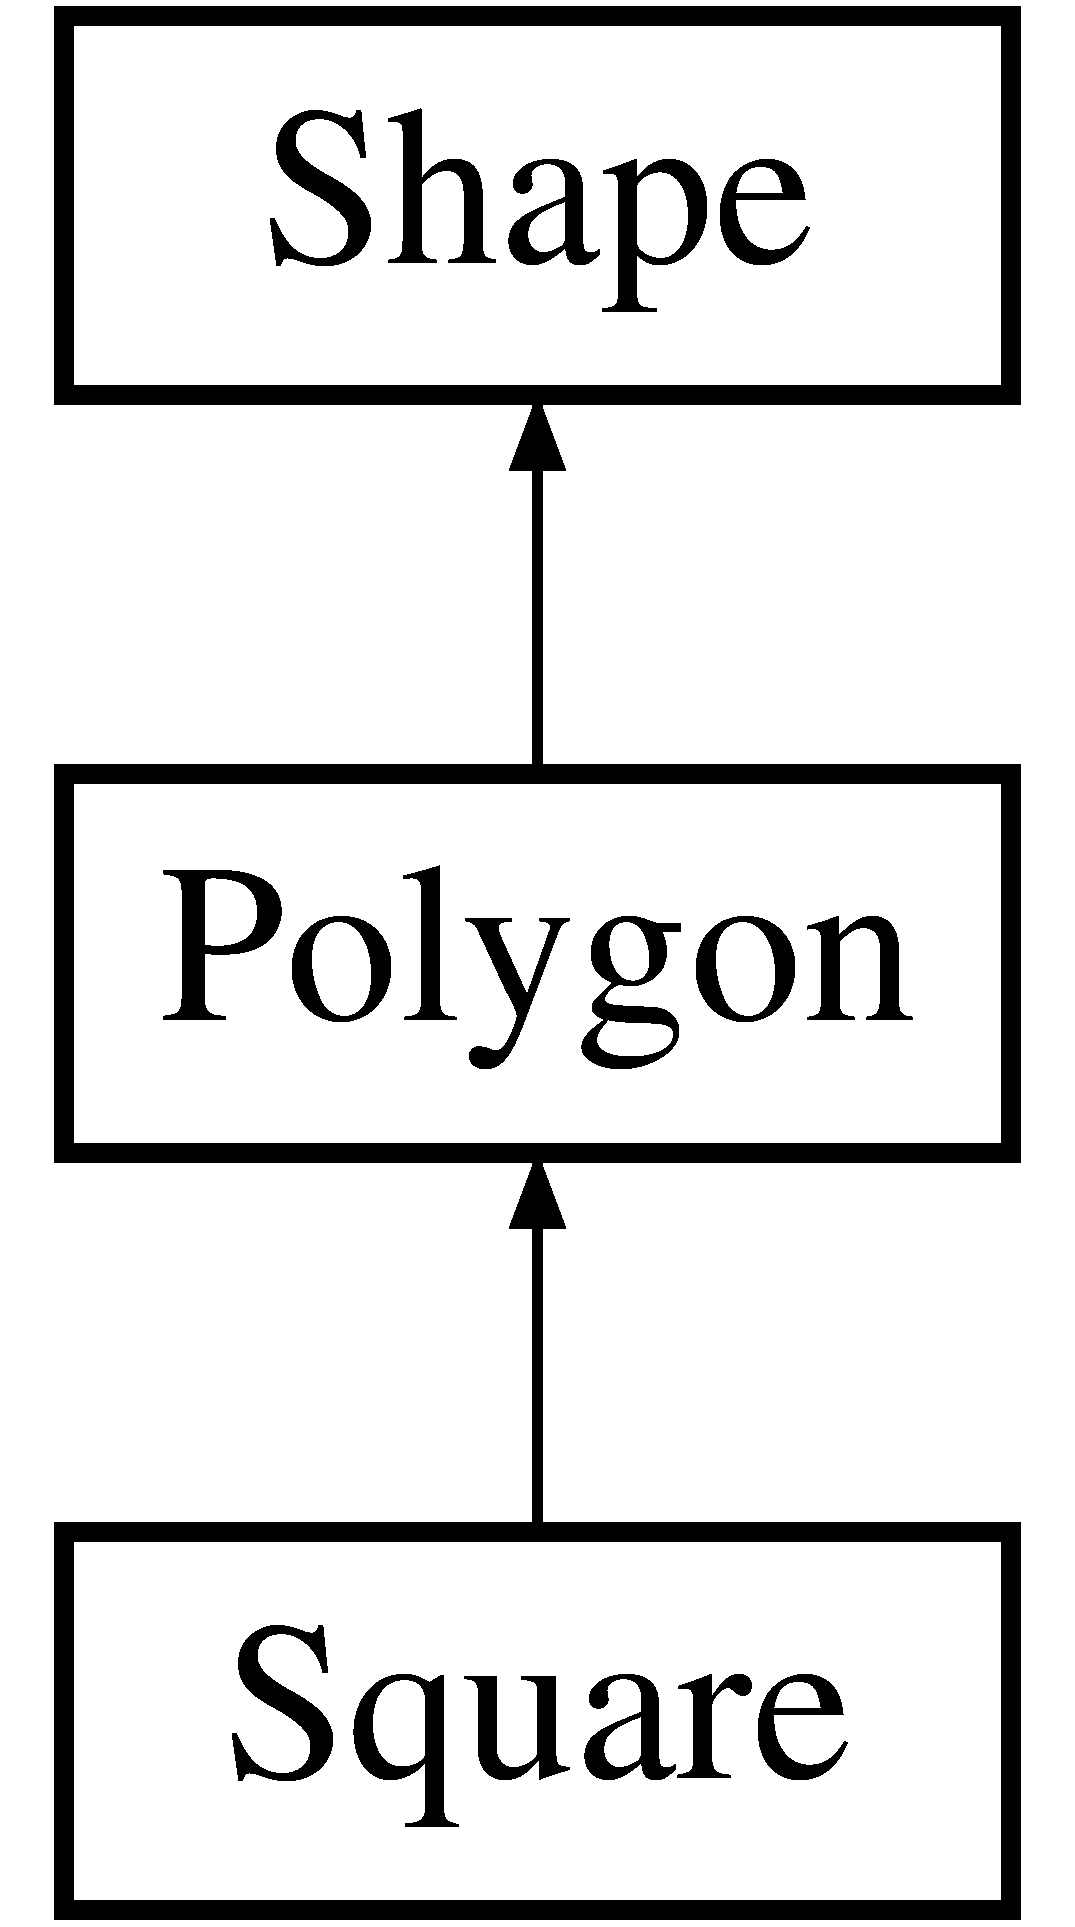
\includegraphics[height=3.000000cm]{class_square}
\end{center}
\end{figure}
\subsection*{Public Member Functions}
\begin{DoxyCompactItemize}
\item 
\hyperlink{class_square_a3dc7ff9aefc2725172b5d3153973d243}{Square} ()
\item 
\hyperlink{class_square_aa8d8831ed45f154396848ef38b99e389}{Square} (int \hyperlink{class_shape_a41e403e73d2949f1a6adfba6032c41ec}{x}, int \hyperlink{class_shape_ac757f715cc5b5681f2c691663ac06f0a}{y}, double side)
\item 
\hyperlink{class_square_a8e4034d486f24636febfaf2235b40834}{Square} (double side)
\end{DoxyCompactItemize}
\subsection*{Additional Inherited Members}


\subsection{Detailed Description}


Definition at line 71 of file polygon.\+h.



\subsection{Constructor \& Destructor Documentation}
\hypertarget{class_square_a3dc7ff9aefc2725172b5d3153973d243}{}\index{Square@{Square}!Square@{Square}}
\index{Square@{Square}!Square@{Square}}
\subsubsection[{Square()}]{\setlength{\rightskip}{0pt plus 5cm}Square\+::\+Square (
\begin{DoxyParamCaption}
{}
\end{DoxyParamCaption}
)\hspace{0.3cm}{\ttfamily [inline]}}\label{class_square_a3dc7ff9aefc2725172b5d3153973d243}


Definition at line 74 of file polygon.\+h.

\hypertarget{class_square_aa8d8831ed45f154396848ef38b99e389}{}\index{Square@{Square}!Square@{Square}}
\index{Square@{Square}!Square@{Square}}
\subsubsection[{Square(int x, int y, double side)}]{\setlength{\rightskip}{0pt plus 5cm}Square\+::\+Square (
\begin{DoxyParamCaption}
\item[{int}]{x, }
\item[{int}]{y, }
\item[{double}]{side}
\end{DoxyParamCaption}
)\hspace{0.3cm}{\ttfamily [inline]}}\label{class_square_aa8d8831ed45f154396848ef38b99e389}


Definition at line 75 of file polygon.\+h.

\hypertarget{class_square_a8e4034d486f24636febfaf2235b40834}{}\index{Square@{Square}!Square@{Square}}
\index{Square@{Square}!Square@{Square}}
\subsubsection[{Square(double side)}]{\setlength{\rightskip}{0pt plus 5cm}Square\+::\+Square (
\begin{DoxyParamCaption}
\item[{double}]{side}
\end{DoxyParamCaption}
)\hspace{0.3cm}{\ttfamily [inline]}}\label{class_square_a8e4034d486f24636febfaf2235b40834}


Definition at line 76 of file polygon.\+h.



The documentation for this class was generated from the following file\+:\begin{DoxyCompactItemize}
\item 
\hyperlink{polygon_8h}{polygon.\+h}\end{DoxyCompactItemize}

\hypertarget{class_star}{}\section{Star Class Reference}
\label{class_star}\index{Star@{Star}}


{\ttfamily \#include $<$star.\+h$>$}

Inheritance diagram for Star\+:\begin{figure}[H]
\begin{center}
\leavevmode
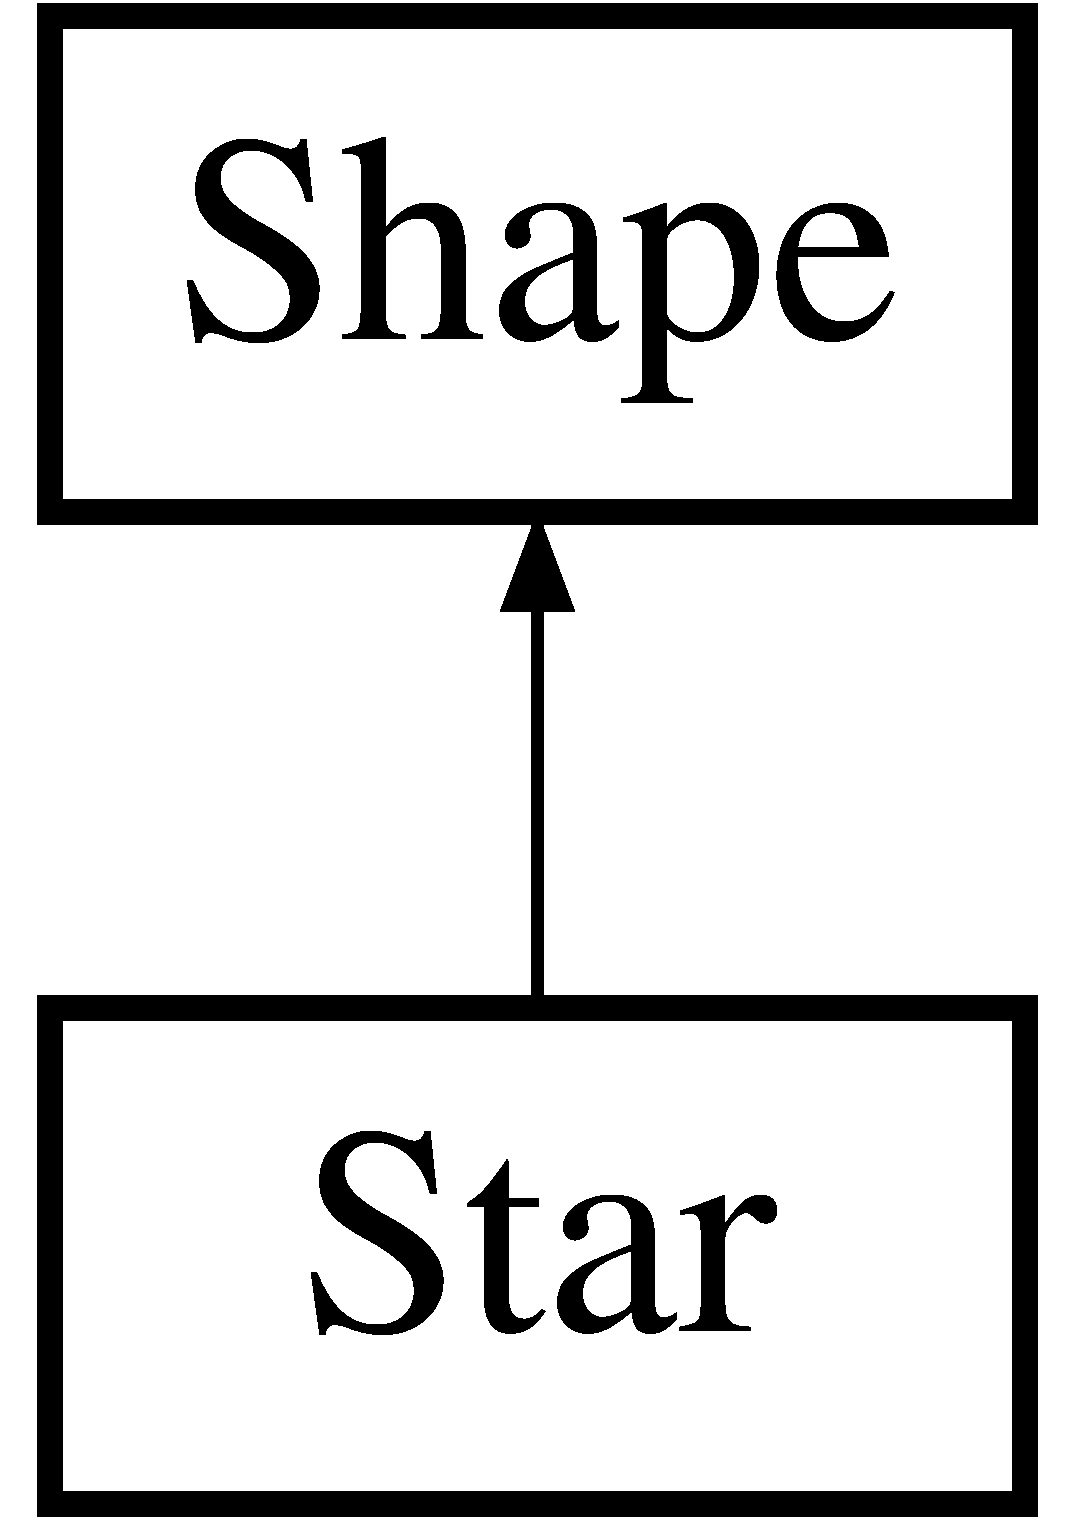
\includegraphics[height=2.000000cm]{class_star}
\end{center}
\end{figure}
\subsection*{Public Member Functions}
\begin{DoxyCompactItemize}
\item 
\hyperlink{class_star_ac174c691c269196c47324a13c3c9f903}{Star} ()
\item 
\hyperlink{class_star_a7f70657eb4be758ec1625e96fbca2133}{Star} (int \hyperlink{class_shape_a41e403e73d2949f1a6adfba6032c41ec}{x}, int \hyperlink{class_shape_ac757f715cc5b5681f2c691663ac06f0a}{y}, int n, double o\+Radius, double i\+Radius)
\item 
\hyperlink{class_star_ac85c92d7f8092da3f5389de37bce8aaa}{Star} (int n, double o\+Radius, double i\+Radius)
\item 
string \hyperlink{class_star_ae0187621a33e5b704f92c77089250316}{draw} () const 
\begin{DoxyCompactList}\small\item\em generate ps code for shape \end{DoxyCompactList}\item 
string \hyperlink{class_star_abb1a219aa29c63205f1e23a056aae521}{draw} (int \hyperlink{class_shape_a41e403e73d2949f1a6adfba6032c41ec}{x}, int \hyperlink{class_shape_ac757f715cc5b5681f2c691663ac06f0a}{y}) const 
\begin{DoxyCompactList}\small\item\em generate ps code for shape \end{DoxyCompactList}\item 
double \hyperlink{class_star_a4bdd108f370f19dc64e9b77df356e1b4}{outer\+Radius} ()
\item 
double \hyperlink{class_star_a35844d0e29a4ad7d5f8ff110832ab31b}{inner\+Radius} ()
\end{DoxyCompactItemize}
\subsection*{Additional Inherited Members}


\subsection{Detailed Description}


Definition at line 14 of file star.\+h.



\subsection{Constructor \& Destructor Documentation}
\hypertarget{class_star_ac174c691c269196c47324a13c3c9f903}{}\index{Star@{Star}!Star@{Star}}
\index{Star@{Star}!Star@{Star}}
\subsubsection[{Star()}]{\setlength{\rightskip}{0pt plus 5cm}Star\+::\+Star (
\begin{DoxyParamCaption}
{}
\end{DoxyParamCaption}
)\hspace{0.3cm}{\ttfamily [inline]}}\label{class_star_ac174c691c269196c47324a13c3c9f903}


Definition at line 17 of file star.\+h.

\hypertarget{class_star_a7f70657eb4be758ec1625e96fbca2133}{}\index{Star@{Star}!Star@{Star}}
\index{Star@{Star}!Star@{Star}}
\subsubsection[{Star(int x, int y, int n, double o\+Radius, double i\+Radius)}]{\setlength{\rightskip}{0pt plus 5cm}Star\+::\+Star (
\begin{DoxyParamCaption}
\item[{int}]{x, }
\item[{int}]{y, }
\item[{int}]{n, }
\item[{double}]{o\+Radius, }
\item[{double}]{i\+Radius}
\end{DoxyParamCaption}
)\hspace{0.3cm}{\ttfamily [inline]}}\label{class_star_a7f70657eb4be758ec1625e96fbca2133}


Definition at line 18 of file star.\+h.

\hypertarget{class_star_ac85c92d7f8092da3f5389de37bce8aaa}{}\index{Star@{Star}!Star@{Star}}
\index{Star@{Star}!Star@{Star}}
\subsubsection[{Star(int n, double o\+Radius, double i\+Radius)}]{\setlength{\rightskip}{0pt plus 5cm}Star\+::\+Star (
\begin{DoxyParamCaption}
\item[{int}]{n, }
\item[{double}]{o\+Radius, }
\item[{double}]{i\+Radius}
\end{DoxyParamCaption}
)\hspace{0.3cm}{\ttfamily [inline]}}\label{class_star_ac85c92d7f8092da3f5389de37bce8aaa}


Definition at line 19 of file star.\+h.



\subsection{Member Function Documentation}
\hypertarget{class_star_ae0187621a33e5b704f92c77089250316}{}\index{Star@{Star}!draw@{draw}}
\index{draw@{draw}!Star@{Star}}
\subsubsection[{draw() const }]{\setlength{\rightskip}{0pt plus 5cm}string Star\+::draw (
\begin{DoxyParamCaption}
{}
\end{DoxyParamCaption}
) const\hspace{0.3cm}{\ttfamily [virtual]}}\label{class_star_ae0187621a33e5b704f92c77089250316}


generate ps code for shape 

generate ps code for drawing shape at default location \begin{DoxyReturn}{Returns}
string containing ps code for drawing shape at default location 
\end{DoxyReturn}


Reimplemented from \hyperlink{class_shape_a8405e352e8bbbdd173fd89065d63a80b}{Shape}.



Definition at line 11 of file star.\+cpp.

\hypertarget{class_star_abb1a219aa29c63205f1e23a056aae521}{}\index{Star@{Star}!draw@{draw}}
\index{draw@{draw}!Star@{Star}}
\subsubsection[{draw(int x, int y) const }]{\setlength{\rightskip}{0pt plus 5cm}string Star\+::draw (
\begin{DoxyParamCaption}
\item[{int}]{x, }
\item[{int}]{y}
\end{DoxyParamCaption}
) const\hspace{0.3cm}{\ttfamily [virtual]}}\label{class_star_abb1a219aa29c63205f1e23a056aae521}


generate ps code for shape 

generate ps code for drawing shape at specified coordinates


\begin{DoxyParams}{Parameters}
{\em x} & x position for center of shape\textquotesingle{}s desired location \\
\hline
{\em y} & y position for center of shape\textquotesingle{}s desired location\\
\hline
\end{DoxyParams}
\begin{DoxyReturn}{Returns}
string containing ps code for drawing shape at specified location 
\end{DoxyReturn}


Reimplemented from \hyperlink{class_shape_af26d06a96ece90a563795ec571451eb1}{Shape}.



Definition at line 15 of file star.\+cpp.

\hypertarget{class_star_a35844d0e29a4ad7d5f8ff110832ab31b}{}\index{Star@{Star}!inner\+Radius@{inner\+Radius}}
\index{inner\+Radius@{inner\+Radius}!Star@{Star}}
\subsubsection[{inner\+Radius()}]{\setlength{\rightskip}{0pt plus 5cm}double Star\+::inner\+Radius (
\begin{DoxyParamCaption}
{}
\end{DoxyParamCaption}
)}\label{class_star_a35844d0e29a4ad7d5f8ff110832ab31b}
\hypertarget{class_star_a4bdd108f370f19dc64e9b77df356e1b4}{}\index{Star@{Star}!outer\+Radius@{outer\+Radius}}
\index{outer\+Radius@{outer\+Radius}!Star@{Star}}
\subsubsection[{outer\+Radius()}]{\setlength{\rightskip}{0pt plus 5cm}double Star\+::outer\+Radius (
\begin{DoxyParamCaption}
{}
\end{DoxyParamCaption}
)}\label{class_star_a4bdd108f370f19dc64e9b77df356e1b4}


The documentation for this class was generated from the following files\+:\begin{DoxyCompactItemize}
\item 
\hyperlink{star_8h}{star.\+h}\item 
\hyperlink{star_8cpp}{star.\+cpp}\end{DoxyCompactItemize}

\hypertarget{class_triangle}{}\section{Triangle Class Reference}
\label{class_triangle}\index{Triangle@{Triangle}}


{\ttfamily \#include $<$polygon.\+h$>$}

Inheritance diagram for Triangle\+:\begin{figure}[H]
\begin{center}
\leavevmode
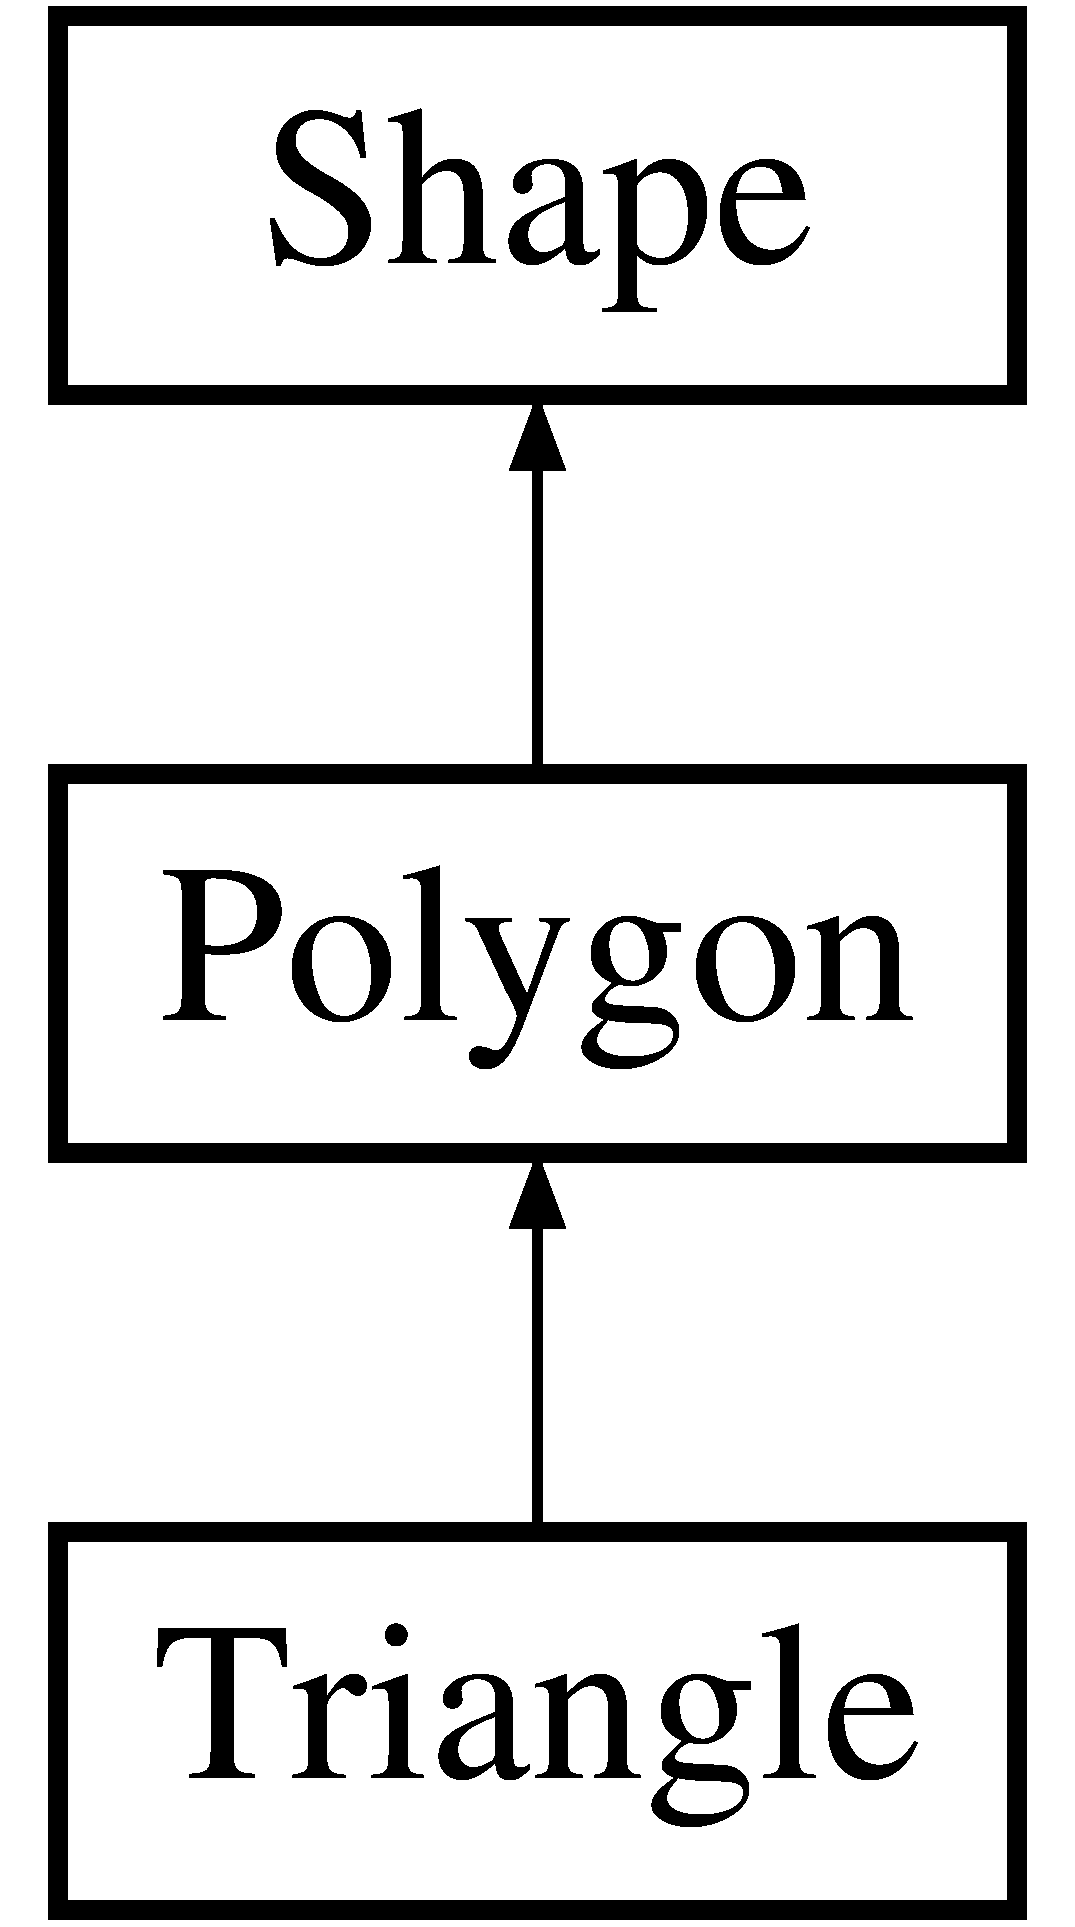
\includegraphics[height=3.000000cm]{class_triangle}
\end{center}
\end{figure}
\subsection*{Public Member Functions}
\begin{DoxyCompactItemize}
\item 
\hyperlink{class_triangle_aaefe4ed500c07918d30c6f0e286332c5}{Triangle} ()
\item 
\hyperlink{class_triangle_a026fe60b6825f39eb8c582ab13032582}{Triangle} (int \hyperlink{class_shape_a41e403e73d2949f1a6adfba6032c41ec}{x}, int \hyperlink{class_shape_ac757f715cc5b5681f2c691663ac06f0a}{y}, double side)
\item 
\hyperlink{class_triangle_a55a9c6195c3f384f3b21b90a80ddc5c3}{Triangle} (double side)
\end{DoxyCompactItemize}
\subsection*{Additional Inherited Members}


\subsection{Detailed Description}


Definition at line 60 of file polygon.\+h.



\subsection{Constructor \& Destructor Documentation}
\hypertarget{class_triangle_aaefe4ed500c07918d30c6f0e286332c5}{}\index{Triangle@{Triangle}!Triangle@{Triangle}}
\index{Triangle@{Triangle}!Triangle@{Triangle}}
\subsubsection[{Triangle()}]{\setlength{\rightskip}{0pt plus 5cm}Triangle\+::\+Triangle (
\begin{DoxyParamCaption}
{}
\end{DoxyParamCaption}
)\hspace{0.3cm}{\ttfamily [inline]}}\label{class_triangle_aaefe4ed500c07918d30c6f0e286332c5}


Definition at line 63 of file polygon.\+h.

\hypertarget{class_triangle_a026fe60b6825f39eb8c582ab13032582}{}\index{Triangle@{Triangle}!Triangle@{Triangle}}
\index{Triangle@{Triangle}!Triangle@{Triangle}}
\subsubsection[{Triangle(int x, int y, double side)}]{\setlength{\rightskip}{0pt plus 5cm}Triangle\+::\+Triangle (
\begin{DoxyParamCaption}
\item[{int}]{x, }
\item[{int}]{y, }
\item[{double}]{side}
\end{DoxyParamCaption}
)\hspace{0.3cm}{\ttfamily [inline]}}\label{class_triangle_a026fe60b6825f39eb8c582ab13032582}


Definition at line 64 of file polygon.\+h.

\hypertarget{class_triangle_a55a9c6195c3f384f3b21b90a80ddc5c3}{}\index{Triangle@{Triangle}!Triangle@{Triangle}}
\index{Triangle@{Triangle}!Triangle@{Triangle}}
\subsubsection[{Triangle(double side)}]{\setlength{\rightskip}{0pt plus 5cm}Triangle\+::\+Triangle (
\begin{DoxyParamCaption}
\item[{double}]{side}
\end{DoxyParamCaption}
)\hspace{0.3cm}{\ttfamily [inline]}}\label{class_triangle_a55a9c6195c3f384f3b21b90a80ddc5c3}


Definition at line 65 of file polygon.\+h.



The documentation for this class was generated from the following file\+:\begin{DoxyCompactItemize}
\item 
\hyperlink{polygon_8h}{polygon.\+h}\end{DoxyCompactItemize}

\hypertarget{class_vertical}{}\section{Vertical Class Reference}
\label{class_vertical}\index{Vertical@{Vertical}}


{\ttfamily \#include $<$layered.\+h$>$}

Inheritance diagram for Vertical\+:\begin{figure}[H]
\begin{center}
\leavevmode
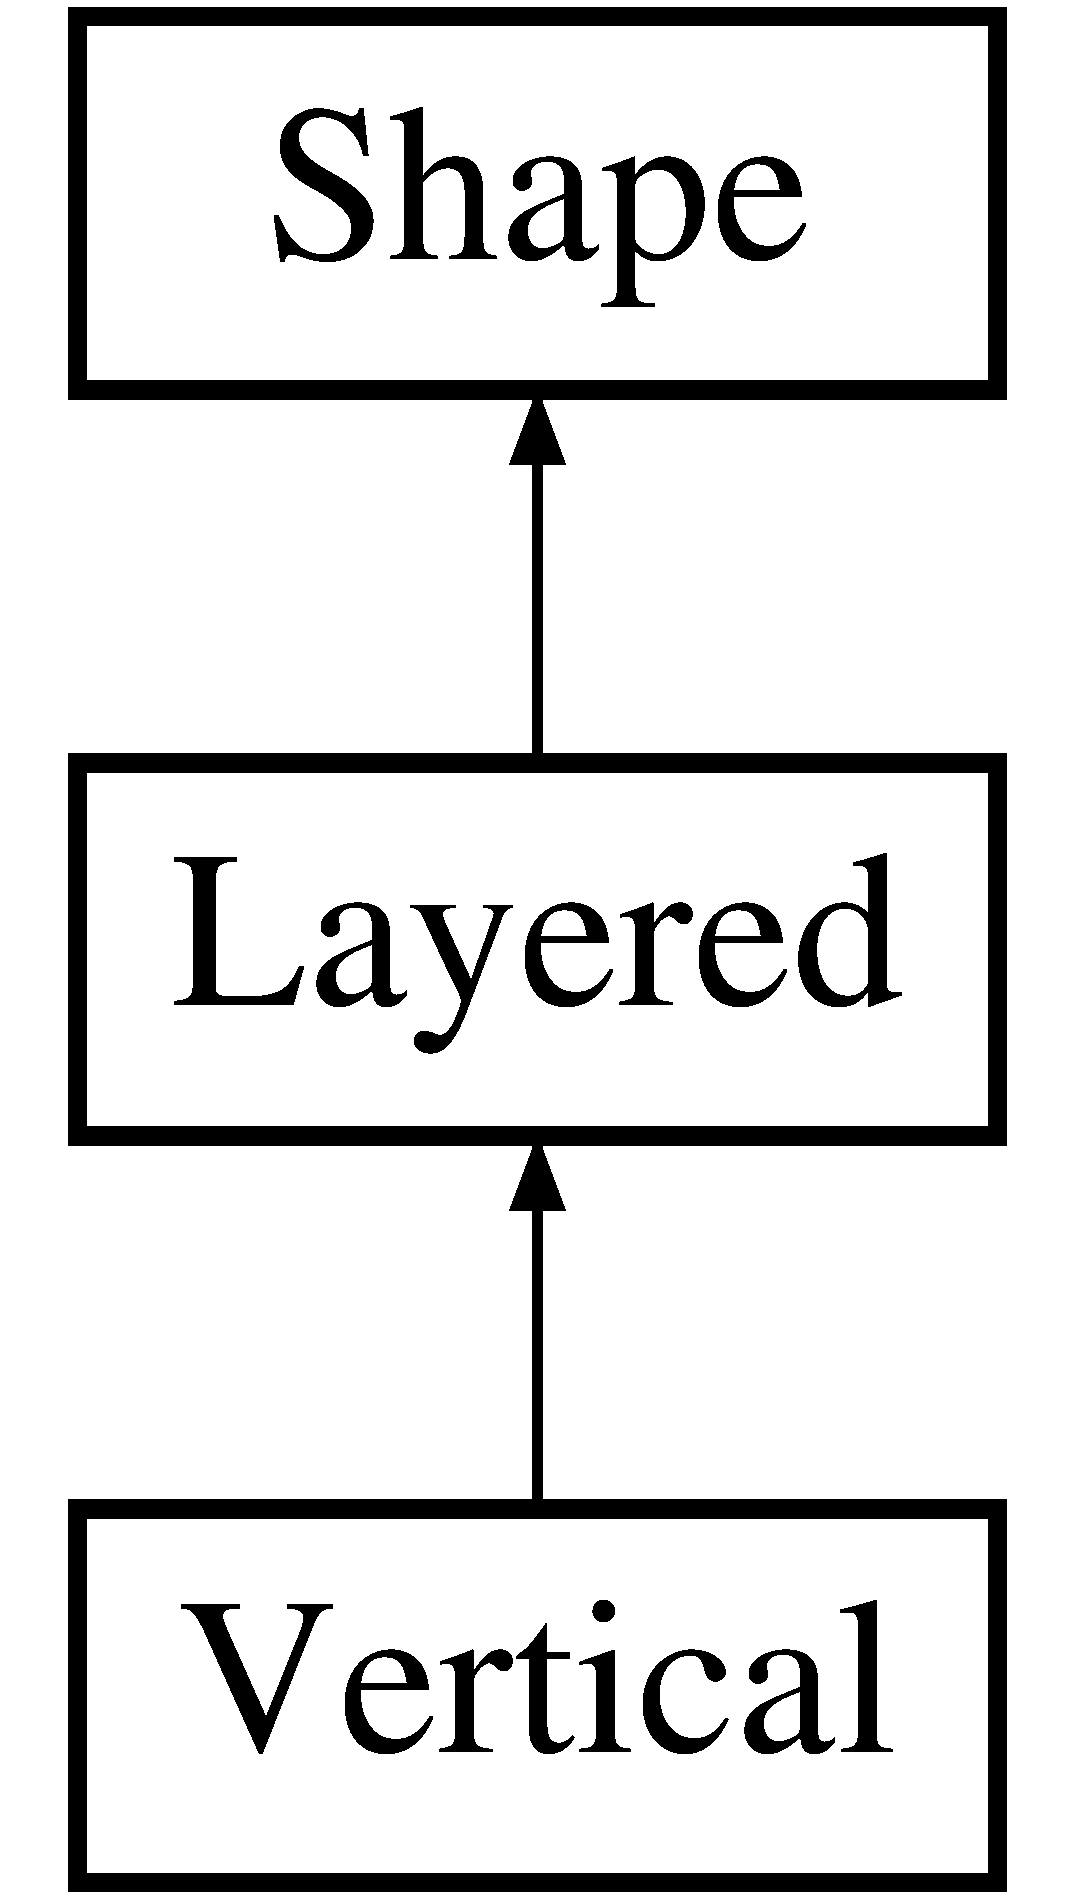
\includegraphics[height=3.000000cm]{class_vertical}
\end{center}
\end{figure}
\subsection*{Public Member Functions}
\begin{DoxyCompactItemize}
\item 
\hyperlink{class_vertical_abe7fe115a8ff6300a0e60fab51f4da7e}{Vertical} ()
\item 
\hyperlink{class_vertical_a534fca34871e38a252b40acf94e05dbf}{Vertical} (int \hyperlink{class_shape_a41e403e73d2949f1a6adfba6032c41ec}{x}, int \hyperlink{class_shape_ac757f715cc5b5681f2c691663ac06f0a}{y}, initializer\+\_\+list$<$ \hyperlink{class_shape}{Shape} $\ast$ $>$ shapes)
\begin{DoxyCompactList}\small\item\em \hyperlink{class_vertical}{Vertical} constructor. \end{DoxyCompactList}\item 
\hyperlink{class_vertical_a3356dc6b2454dea361e08224b1bb187c}{Vertical} (initializer\+\_\+list$<$ \hyperlink{class_shape}{Shape} $\ast$ $>$ shapes)
\item 
string \hyperlink{class_vertical_a778fd2aa48afcf255b75413e29613ebb}{draw} () const 
\begin{DoxyCompactList}\small\item\em generate ps code for shape \end{DoxyCompactList}\item 
string \hyperlink{class_vertical_a9be329f986230ccaa35ec7f63553d658}{draw} (int \hyperlink{class_shape_a41e403e73d2949f1a6adfba6032c41ec}{x}, int \hyperlink{class_shape_ac757f715cc5b5681f2c691663ac06f0a}{y}) const 
\begin{DoxyCompactList}\small\item\em generate ps code for shape \end{DoxyCompactList}\end{DoxyCompactItemize}
\subsection*{Additional Inherited Members}


\subsection{Detailed Description}


Definition at line 46 of file layered.\+h.



\subsection{Constructor \& Destructor Documentation}
\hypertarget{class_vertical_abe7fe115a8ff6300a0e60fab51f4da7e}{}\index{Vertical@{Vertical}!Vertical@{Vertical}}
\index{Vertical@{Vertical}!Vertical@{Vertical}}
\subsubsection[{Vertical()}]{\setlength{\rightskip}{0pt plus 5cm}Vertical\+::\+Vertical (
\begin{DoxyParamCaption}
{}
\end{DoxyParamCaption}
)\hspace{0.3cm}{\ttfamily [inline]}}\label{class_vertical_abe7fe115a8ff6300a0e60fab51f4da7e}


Definition at line 49 of file layered.\+h.

\hypertarget{class_vertical_a534fca34871e38a252b40acf94e05dbf}{}\index{Vertical@{Vertical}!Vertical@{Vertical}}
\index{Vertical@{Vertical}!Vertical@{Vertical}}
\subsubsection[{Vertical(int x, int y, initializer\+\_\+list$<$ Shape $\ast$ $>$ shapes)}]{\setlength{\rightskip}{0pt plus 5cm}Vertical\+::\+Vertical (
\begin{DoxyParamCaption}
\item[{int}]{x, }
\item[{int}]{y, }
\item[{initializer\+\_\+list$<$ {\bf Shape} $\ast$ $>$}]{shapes}
\end{DoxyParamCaption}
)}\label{class_vertical_a534fca34871e38a252b40acf94e05dbf}


\hyperlink{class_vertical}{Vertical} constructor. 

constructs a \hyperlink{class_vertical}{Vertical} shape from a list of Shapes


\begin{DoxyParams}{Parameters}
{\em x} & x position of center \\
\hline
{\em y} & y position of center \\
\hline
{\em shapes} & list of pointers to Shapes \\
\hline
\end{DoxyParams}


Definition at line 94 of file layered.\+cpp.

\hypertarget{class_vertical_a3356dc6b2454dea361e08224b1bb187c}{}\index{Vertical@{Vertical}!Vertical@{Vertical}}
\index{Vertical@{Vertical}!Vertical@{Vertical}}
\subsubsection[{Vertical(initializer\+\_\+list$<$ Shape $\ast$ $>$ shapes)}]{\setlength{\rightskip}{0pt plus 5cm}Vertical\+::\+Vertical (
\begin{DoxyParamCaption}
\item[{initializer\+\_\+list$<$ {\bf Shape} $\ast$ $>$}]{shapes}
\end{DoxyParamCaption}
)\hspace{0.3cm}{\ttfamily [inline]}}\label{class_vertical_a3356dc6b2454dea361e08224b1bb187c}


Definition at line 51 of file layered.\+h.



\subsection{Member Function Documentation}
\hypertarget{class_vertical_a778fd2aa48afcf255b75413e29613ebb}{}\index{Vertical@{Vertical}!draw@{draw}}
\index{draw@{draw}!Vertical@{Vertical}}
\subsubsection[{draw() const }]{\setlength{\rightskip}{0pt plus 5cm}string Vertical\+::draw (
\begin{DoxyParamCaption}
{}
\end{DoxyParamCaption}
) const\hspace{0.3cm}{\ttfamily [virtual]}}\label{class_vertical_a778fd2aa48afcf255b75413e29613ebb}


generate ps code for shape 

generate ps code for drawing shape at default location \begin{DoxyReturn}{Returns}
string containing ps code for drawing shape at default location 
\end{DoxyReturn}


Reimplemented from \hyperlink{class_layered_a968cd141e61eb039b997352a318dcae0}{Layered}.



Definition at line 104 of file layered.\+cpp.

\hypertarget{class_vertical_a9be329f986230ccaa35ec7f63553d658}{}\index{Vertical@{Vertical}!draw@{draw}}
\index{draw@{draw}!Vertical@{Vertical}}
\subsubsection[{draw(int x, int y) const }]{\setlength{\rightskip}{0pt plus 5cm}string Vertical\+::draw (
\begin{DoxyParamCaption}
\item[{int}]{x, }
\item[{int}]{y}
\end{DoxyParamCaption}
) const\hspace{0.3cm}{\ttfamily [virtual]}}\label{class_vertical_a9be329f986230ccaa35ec7f63553d658}


generate ps code for shape 

generate ps code for drawing shape at specified coordinates


\begin{DoxyParams}{Parameters}
{\em x} & x position for center of shape\textquotesingle{}s desired location \\
\hline
{\em y} & y position for center of shape\textquotesingle{}s desired location\\
\hline
\end{DoxyParams}
\begin{DoxyReturn}{Returns}
string containing ps code for drawing shape at specified location 
\end{DoxyReturn}


Reimplemented from \hyperlink{class_layered_a6eb564ff0646b26fdd4175856b1a0815}{Layered}.



Definition at line 108 of file layered.\+cpp.



The documentation for this class was generated from the following files\+:\begin{DoxyCompactItemize}
\item 
\hyperlink{layered_8h}{layered.\+h}\item 
\hyperlink{layered_8cpp}{layered.\+cpp}\end{DoxyCompactItemize}

\chapter{File Documentation}
\hypertarget{circle_8cpp}{}\section{circle.\+cpp File Reference}
\label{circle_8cpp}\index{circle.\+cpp@{circle.\+cpp}}
{\ttfamily \#include \char`\"{}circle.\+h\char`\"{}}\\*

\hypertarget{circle_8h}{}\section{circle.\+h File Reference}
\label{circle_8h}\index{circle.\+h@{circle.\+h}}
{\ttfamily \#include \char`\"{}shape.\+h\char`\"{}}\\*
\subsection*{Classes}
\begin{DoxyCompactItemize}
\item 
class \hyperlink{class_circle}{Circle}
\end{DoxyCompactItemize}

\hypertarget{layered_8cpp}{}\section{layered.\+cpp File Reference}
\label{layered_8cpp}\index{layered.\+cpp@{layered.\+cpp}}
{\ttfamily \#include \char`\"{}layered.\+h\char`\"{}}\\*

\hypertarget{layered_8h}{}\section{layered.\+h File Reference}
\label{layered_8h}\index{layered.\+h@{layered.\+h}}
{\ttfamily \#include $<$initializer\+\_\+list$>$}\\*
{\ttfamily \#include \char`\"{}shape.\+h\char`\"{}}\\*
\subsection*{Classes}
\begin{DoxyCompactItemize}
\item 
class \hyperlink{class_layered}{Layered}
\item 
class \hyperlink{class_horizontal}{Horizontal}
\item 
class \hyperlink{class_vertical}{Vertical}
\end{DoxyCompactItemize}

\hypertarget{main_8cpp}{}\section{main.\+cpp File Reference}
\label{main_8cpp}\index{main.\+cpp@{main.\+cpp}}
{\ttfamily \#include \char`\"{}shape.\+h\char`\"{}}\\*
{\ttfamily \#include \char`\"{}circle.\+h\char`\"{}}\\*
{\ttfamily \#include \char`\"{}polygon.\+h\char`\"{}}\\*
{\ttfamily \#include \char`\"{}rectangle.\+h\char`\"{}}\\*
{\ttfamily \#include \char`\"{}spacer.\+h\char`\"{}}\\*
{\ttfamily \#include \char`\"{}layered.\+h\char`\"{}}\\*
{\ttfamily \#include \char`\"{}rotate.\+h\char`\"{}}\\*
{\ttfamily \#include \char`\"{}scaled.\+h\char`\"{}}\\*
{\ttfamily \#include \char`\"{}utils.\+h\char`\"{}}\\*
{\ttfamily \#include \char`\"{}star.\+h\char`\"{}}\\*
{\ttfamily \#include $<$typeinfo$>$}\\*
{\ttfamily \#include $<$iostream$>$}\\*
\subsection*{Functions}
\begin{DoxyCompactItemize}
\item 
int \hyperlink{main_8cpp_ae66f6b31b5ad750f1fe042a706a4e3d4}{main} ()
\end{DoxyCompactItemize}


\subsection{Function Documentation}
\hypertarget{main_8cpp_ae66f6b31b5ad750f1fe042a706a4e3d4}{}\index{main.\+cpp@{main.\+cpp}!main@{main}}
\index{main@{main}!main.\+cpp@{main.\+cpp}}
\subsubsection[{main()}]{\setlength{\rightskip}{0pt plus 5cm}int main (
\begin{DoxyParamCaption}
{}
\end{DoxyParamCaption}
)}\label{main_8cpp_ae66f6b31b5ad750f1fe042a706a4e3d4}


Definition at line 33 of file main.\+cpp.


\hypertarget{polygon_8cpp}{}\section{polygon.\+cpp File Reference}
\label{polygon_8cpp}\index{polygon.\+cpp@{polygon.\+cpp}}
{\ttfamily \#include \char`\"{}polygon.\+h\char`\"{}}\\*

\hypertarget{polygon_8h}{}\section{polygon.\+h File Reference}
\label{polygon_8h}\index{polygon.\+h@{polygon.\+h}}
{\ttfamily \#include \char`\"{}shape.\+h\char`\"{}}\\*
\subsection*{Classes}
\begin{DoxyCompactItemize}
\item 
class \hyperlink{class_polygon}{Polygon}
\item 
class \hyperlink{class_triangle}{Triangle}
\item 
class \hyperlink{class_square}{Square}
\end{DoxyCompactItemize}

\hypertarget{rectangle_8cpp}{}\section{rectangle.\+cpp File Reference}
\label{rectangle_8cpp}\index{rectangle.\+cpp@{rectangle.\+cpp}}
{\ttfamily \#include \char`\"{}rectangle.\+h\char`\"{}}\\*

\hypertarget{rectangle_8h}{}\section{rectangle.\+h File Reference}
\label{rectangle_8h}\index{rectangle.\+h@{rectangle.\+h}}
{\ttfamily \#include \char`\"{}shape.\+h\char`\"{}}\\*
{\ttfamily \#include $<$sstream$>$}\\*
\subsection*{Classes}
\begin{DoxyCompactItemize}
\item 
class \hyperlink{class_rectangle}{Rectangle}
\end{DoxyCompactItemize}

\hypertarget{rotate_8cpp}{}\section{rotate.\+cpp File Reference}
\label{rotate_8cpp}\index{rotate.\+cpp@{rotate.\+cpp}}
{\ttfamily \#include \char`\"{}rotate.\+h\char`\"{}}\\*

\hypertarget{rotate_8h}{}\section{rotate.\+h File Reference}
\label{rotate_8h}\index{rotate.\+h@{rotate.\+h}}
{\ttfamily \#include \char`\"{}shape.\+h\char`\"{}}\\*
\subsection*{Classes}
\begin{DoxyCompactItemize}
\item 
class \hyperlink{class_rotated}{Rotated}
\end{DoxyCompactItemize}

\hypertarget{scaled_8cpp}{}\section{scaled.\+cpp File Reference}
\label{scaled_8cpp}\index{scaled.\+cpp@{scaled.\+cpp}}
{\ttfamily \#include \char`\"{}scaled.\+h\char`\"{}}\\*

\hypertarget{scaled_8h}{}\section{scaled.\+h File Reference}
\label{scaled_8h}\index{scaled.\+h@{scaled.\+h}}
{\ttfamily \#include \char`\"{}shape.\+h\char`\"{}}\\*
\subsection*{Classes}
\begin{DoxyCompactItemize}
\item 
class \hyperlink{class_scaled}{Scaled}
\end{DoxyCompactItemize}

\hypertarget{shape_8cpp}{}\section{shape.\+cpp File Reference}
\label{shape_8cpp}\index{shape.\+cpp@{shape.\+cpp}}
{\ttfamily \#include \char`\"{}shape.\+h\char`\"{}}\\*
\subsection*{Functions}
\begin{DoxyCompactItemize}
\item 
ostream \& \hyperlink{shape_8cpp_ada7f3e97b3113c4725bf7ec7293b5a36}{operator$<$$<$} (ostream \&os, const \hyperlink{class_shape}{Shape} \&shape)
\begin{DoxyCompactList}\small\item\em overloaded output operator \end{DoxyCompactList}\end{DoxyCompactItemize}


\subsection{Function Documentation}
\hypertarget{shape_8cpp_ada7f3e97b3113c4725bf7ec7293b5a36}{}\index{shape.\+cpp@{shape.\+cpp}!operator$<$$<$@{operator$<$$<$}}
\index{operator$<$$<$@{operator$<$$<$}!shape.\+cpp@{shape.\+cpp}}
\subsubsection[{operator$<$$<$(ostream \&os, const Shape \&shape)}]{\setlength{\rightskip}{0pt plus 5cm}ostream\& operator$<$$<$ (
\begin{DoxyParamCaption}
\item[{ostream \&}]{os, }
\item[{const {\bf Shape} \&}]{shape}
\end{DoxyParamCaption}
)}\label{shape_8cpp_ada7f3e97b3113c4725bf7ec7293b5a36}


overloaded output operator 

prints the ps code for drawing the shape to the calling ostream


\begin{DoxyParams}{Parameters}
{\em os} & target ostream, passed implicitly \\
\hline
{\em shape} & \hyperlink{class_shape}{Shape} to print, passed implicitly \\
\hline
\end{DoxyParams}


Definition at line 168 of file shape.\+cpp.


\hypertarget{shape_8h}{}\section{shape.\+h File Reference}
\label{shape_8h}\index{shape.\+h@{shape.\+h}}
{\ttfamily \#include $<$utility$>$}\\*
{\ttfamily \#include $<$string$>$}\\*
{\ttfamily \#include $<$sstream$>$}\\*
{\ttfamily \#include $<$cmath$>$}\\*
{\ttfamily \#include $<$iostream$>$}\\*
{\ttfamily \#include $<$algorithm$>$}\\*
{\ttfamily \#include $<$typeinfo$>$}\\*
{\ttfamily \#include \char`\"{}utils.\+h\char`\"{}}\\*
\subsection*{Classes}
\begin{DoxyCompactItemize}
\item 
class \hyperlink{class_shape}{Shape}
\end{DoxyCompactItemize}
\subsection*{Functions}
\begin{DoxyCompactItemize}
\item 
ostream \& \hyperlink{shape_8h_ada7f3e97b3113c4725bf7ec7293b5a36}{operator$<$$<$} (ostream \&os, const \hyperlink{class_shape}{Shape} \&shape)
\begin{DoxyCompactList}\small\item\em overloaded output operator \end{DoxyCompactList}\end{DoxyCompactItemize}


\subsection{Function Documentation}
\hypertarget{shape_8h_ada7f3e97b3113c4725bf7ec7293b5a36}{}\index{shape.\+h@{shape.\+h}!operator$<$$<$@{operator$<$$<$}}
\index{operator$<$$<$@{operator$<$$<$}!shape.\+h@{shape.\+h}}
\subsubsection[{operator$<$$<$(ostream \&os, const Shape \&shape)}]{\setlength{\rightskip}{0pt plus 5cm}ostream\& operator$<$$<$ (
\begin{DoxyParamCaption}
\item[{ostream \&}]{os, }
\item[{const {\bf Shape} \&}]{shape}
\end{DoxyParamCaption}
)}\label{shape_8h_ada7f3e97b3113c4725bf7ec7293b5a36}


overloaded output operator 

prints the ps code for drawing the shape to the calling ostream


\begin{DoxyParams}{Parameters}
{\em os} & target ostream, passed implicitly \\
\hline
{\em shape} & \hyperlink{class_shape}{Shape} to print, passed implicitly \\
\hline
\end{DoxyParams}


Definition at line 168 of file shape.\+cpp.


\hypertarget{spacer_8cpp}{}\section{spacer.\+cpp File Reference}
\label{spacer_8cpp}\index{spacer.\+cpp@{spacer.\+cpp}}
{\ttfamily \#include \char`\"{}spacer.\+h\char`\"{}}\\*

\hypertarget{spacer_8h}{}\section{spacer.\+h File Reference}
\label{spacer_8h}\index{spacer.\+h@{spacer.\+h}}
{\ttfamily \#include \char`\"{}rectangle.\+h\char`\"{}}\\*
\subsection*{Classes}
\begin{DoxyCompactItemize}
\item 
class \hyperlink{class_spacer}{Spacer}
\end{DoxyCompactItemize}

\hypertarget{star_8cpp}{}\section{star.\+cpp File Reference}
\label{star_8cpp}\index{star.\+cpp@{star.\+cpp}}
{\ttfamily \#include \char`\"{}star.\+h\char`\"{}}\\*

\hypertarget{star_8h}{}\section{star.\+h File Reference}
\label{star_8h}\index{star.\+h@{star.\+h}}
{\ttfamily \#include \char`\"{}shape.\+h\char`\"{}}\\*
\subsection*{Classes}
\begin{DoxyCompactItemize}
\item 
class \hyperlink{class_star}{Star}
\end{DoxyCompactItemize}

\hypertarget{test_8cpp}{}\section{test.\+cpp File Reference}
\label{test_8cpp}\index{test.\+cpp@{test.\+cpp}}
{\ttfamily \#include \char`\"{}catch.\+hpp\char`\"{}}\\*
{\ttfamily \#include $<$random$>$}\\*
{\ttfamily \#include \char`\"{}rectangle.\+h\char`\"{}}\\*
{\ttfamily \#include \char`\"{}polygon.\+h\char`\"{}}\\*
{\ttfamily \#include \char`\"{}spacer.\+h\char`\"{}}\\*
{\ttfamily \#include \char`\"{}circle.\+h\char`\"{}}\\*
{\ttfamily \#include \char`\"{}layered.\+h\char`\"{}}\\*
{\ttfamily \#include \char`\"{}rotate.\+h\char`\"{}}\\*
{\ttfamily \#include \char`\"{}star.\+h\char`\"{}}\\*
{\ttfamily \#include \char`\"{}scaled.\+h\char`\"{}}\\*
\subsection*{Macros}
\begin{DoxyCompactItemize}
\item 
\#define \hyperlink{test_8cpp_a656eb5868e824d59f489f910db438420}{C\+A\+T\+C\+H\+\_\+\+C\+O\+N\+F\+I\+G\+\_\+\+M\+A\+I\+N}
\end{DoxyCompactItemize}
\subsection*{Functions}
\begin{DoxyCompactItemize}
\item 
string \hyperlink{test_8cpp_a05a2cf7a2cccf5ed31896cec5516fb34}{test\+Ps\+Line} (int x, int y)
\item 
string \hyperlink{test_8cpp_ad3ea4dc48b3534885bad21dfca1aecb7}{test\+Ps\+Move} (int x, int y)
\item 
string \hyperlink{test_8cpp_ae11dbf7e8b9a70506cee960cb8eb7ac1}{test\+Ps\+Arc} (int x, int y, double r, int start\+Angle, int end\+Angle)
\item 
string \hyperlink{test_8cpp_a500994bb31d55ee61682a51e9c29515b}{test\+Ps\+Header} (int x, int y)
\item 
string \hyperlink{test_8cpp_a7b69b4bc985b06035fa9e99aa7febb1e}{test\+Ps\+Footer} ()
\item 
double \hyperlink{test_8cpp_a21ad69bdaec05e3c7e33a6c0e2457a52}{test\+Calc\+X} (int k, int n, double l)
\item 
double \hyperlink{test_8cpp_a0f271afc15ce17c857a60f9256262e0f}{test\+Calc\+Y} (int k, int n, double l)
\item 
double \hyperlink{test_8cpp_ac4ac5242bbaf697333ad4c6968e3fa08}{test\+Getwidth} (int sides, double len)
\item 
double \hyperlink{test_8cpp_a52761836fdc054c8b0a8a0d22de206a5}{test\+Get\+Height} (int n, double l)
\item 
double \hyperlink{test_8cpp_a3c22fec146d92745c01395d141de5a58}{test\+Get\+Radius} (int n, double l)
\item 
double \hyperlink{test_8cpp_a895578d3113bd5d5f95d5a9ba23679be}{test\+Get\+Convex\+X} (int k, int n, double r)
\item 
double \hyperlink{test_8cpp_aaa78cb1614d230c465299f64b9673879}{test\+Get\+Convex\+Y} (int k, int n, double r)
\item 
double \hyperlink{test_8cpp_ac60e07c8cc2f232cb260eb17a47a82ad}{test\+Get\+Concave\+X} (int k, int n, double r)
\item 
double \hyperlink{test_8cpp_a2fc1b86165feade40f5e969a5a45742f}{test\+Get\+Concave\+Y} (int k, int n, double r)
\item 
string \hyperlink{test_8cpp_ae9326b802b363d823b82a62ef6f44dcb}{test\+Poly\+Draw} (int x, int y, int sides, double length)
\item 
string \hyperlink{test_8cpp_ab92c281d3f292cc676bb06ebab5df973}{test\+Circle\+Draw} (int x, int y, double radius)
\item 
\hyperlink{test_8cpp_a90116ecd1bf6593f72838013e72e7224}{T\+E\+S\+T\+\_\+\+C\+A\+S\+E} (\char`\"{}Testing utils drawing helpers\char`\"{},\char`\"{}\mbox{[}Utils\mbox{]}\char`\"{})
\item 
\hyperlink{test_8cpp_adc04d9b255824240b506edadf2e1085a}{T\+E\+S\+T\+\_\+\+C\+A\+S\+E} (\char`\"{}Testing Centers\char`\"{},\char`\"{}\mbox{[}Utils\mbox{]}\char`\"{})
\item 
\hyperlink{test_8cpp_a721d97175747b858b178a04d2850d8ad}{T\+E\+S\+T\+\_\+\+C\+A\+S\+E} (\char`\"{}Testing width and height calculations\char`\"{},\char`\"{}\mbox{[}Utils\mbox{]}\char`\"{})
\item 
\hyperlink{test_8cpp_a89ad77ba55c2942dff7df74acb9e62dc}{T\+E\+S\+T\+\_\+\+C\+A\+S\+E} (\char`\"{}Simple \hyperlink{class_shape}{Shape} Default Construction\char`\"{},\char`\"{}\mbox{[}Construction\mbox{]}\char`\"{})
\item 
\hyperlink{test_8cpp_a0db85045df9d5fa1a652c27f0fb40097}{T\+E\+S\+T\+\_\+\+C\+A\+S\+E} (\char`\"{}Polygon Draw\char`\"{},\char`\"{}\mbox{[}\hyperlink{class_polygon}{Polygon}\mbox{]} \mbox{[}draw function\mbox{]}\char`\"{})
\item 
\hyperlink{test_8cpp_abcfdfc36ff5292f8feb49f21c6ab5d63}{T\+E\+S\+T\+\_\+\+C\+A\+S\+E} (\char`\"{}Shape operator $<$$<$\char`\"{},\char`\"{}\mbox{[}\hyperlink{class_shape}{Shape}\mbox{]} \mbox{[}operator $<$$<$\mbox{]}\char`\"{})
\item 
\hyperlink{test_8cpp_ad2be3170398cbf5c9ae07cbb4621b78c}{T\+E\+S\+T\+\_\+\+C\+A\+S\+E} (\char`\"{}Shape operator ()\char`\"{},\char`\"{}\mbox{[}\hyperlink{class_shape}{Shape}\mbox{]} \mbox{[}operator ()\mbox{]}\char`\"{})
\end{DoxyCompactItemize}
\subsection*{Variables}
\begin{DoxyCompactItemize}
\item 
const double \hyperlink{test_8cpp_a1b3972a454d9203b9612da3887e88883}{E\+R\+R\+O\+R} = 0.\+0000001
\end{DoxyCompactItemize}


\subsection{Macro Definition Documentation}
\hypertarget{test_8cpp_a656eb5868e824d59f489f910db438420}{}\index{test.\+cpp@{test.\+cpp}!C\+A\+T\+C\+H\+\_\+\+C\+O\+N\+F\+I\+G\+\_\+\+M\+A\+I\+N@{C\+A\+T\+C\+H\+\_\+\+C\+O\+N\+F\+I\+G\+\_\+\+M\+A\+I\+N}}
\index{C\+A\+T\+C\+H\+\_\+\+C\+O\+N\+F\+I\+G\+\_\+\+M\+A\+I\+N@{C\+A\+T\+C\+H\+\_\+\+C\+O\+N\+F\+I\+G\+\_\+\+M\+A\+I\+N}!test.\+cpp@{test.\+cpp}}
\subsubsection[{C\+A\+T\+C\+H\+\_\+\+C\+O\+N\+F\+I\+G\+\_\+\+M\+A\+I\+N}]{\setlength{\rightskip}{0pt plus 5cm}\#define C\+A\+T\+C\+H\+\_\+\+C\+O\+N\+F\+I\+G\+\_\+\+M\+A\+I\+N}\label{test_8cpp_a656eb5868e824d59f489f910db438420}


Definition at line 1 of file test.\+cpp.



\subsection{Function Documentation}
\hypertarget{test_8cpp_a90116ecd1bf6593f72838013e72e7224}{}\index{test.\+cpp@{test.\+cpp}!T\+E\+S\+T\+\_\+\+C\+A\+S\+E@{T\+E\+S\+T\+\_\+\+C\+A\+S\+E}}
\index{T\+E\+S\+T\+\_\+\+C\+A\+S\+E@{T\+E\+S\+T\+\_\+\+C\+A\+S\+E}!test.\+cpp@{test.\+cpp}}
\subsubsection[{T\+E\+S\+T\+\_\+\+C\+A\+S\+E(""Testing utils drawing helpers"",""[Utils]"")}]{\setlength{\rightskip}{0pt plus 5cm}T\+E\+S\+T\+\_\+\+C\+A\+S\+E (
\begin{DoxyParamCaption}
\item[{\char`\"{}Testing utils drawing helpers\char`\"{}}]{, }
\item[{\char`\"{}\char`\"{}}]{\mbox{[}\+Utils\mbox{]}}
\end{DoxyParamCaption}
)}\label{test_8cpp_a90116ecd1bf6593f72838013e72e7224}


Definition at line 150 of file test.\+cpp.

\hypertarget{test_8cpp_adc04d9b255824240b506edadf2e1085a}{}\index{test.\+cpp@{test.\+cpp}!T\+E\+S\+T\+\_\+\+C\+A\+S\+E@{T\+E\+S\+T\+\_\+\+C\+A\+S\+E}}
\index{T\+E\+S\+T\+\_\+\+C\+A\+S\+E@{T\+E\+S\+T\+\_\+\+C\+A\+S\+E}!test.\+cpp@{test.\+cpp}}
\subsubsection[{T\+E\+S\+T\+\_\+\+C\+A\+S\+E(""Testing Centers"",""[Utils]"")}]{\setlength{\rightskip}{0pt plus 5cm}T\+E\+S\+T\+\_\+\+C\+A\+S\+E (
\begin{DoxyParamCaption}
\item[{\char`\"{}Testing Centers\char`\"{}}]{, }
\item[{\char`\"{}\char`\"{}}]{\mbox{[}\+Utils\mbox{]}}
\end{DoxyParamCaption}
)}\label{test_8cpp_adc04d9b255824240b506edadf2e1085a}


Definition at line 211 of file test.\+cpp.

\hypertarget{test_8cpp_a721d97175747b858b178a04d2850d8ad}{}\index{test.\+cpp@{test.\+cpp}!T\+E\+S\+T\+\_\+\+C\+A\+S\+E@{T\+E\+S\+T\+\_\+\+C\+A\+S\+E}}
\index{T\+E\+S\+T\+\_\+\+C\+A\+S\+E@{T\+E\+S\+T\+\_\+\+C\+A\+S\+E}!test.\+cpp@{test.\+cpp}}
\subsubsection[{T\+E\+S\+T\+\_\+\+C\+A\+S\+E(""Testing width and height calculations"",""[Utils]"")}]{\setlength{\rightskip}{0pt plus 5cm}T\+E\+S\+T\+\_\+\+C\+A\+S\+E (
\begin{DoxyParamCaption}
\item[{\char`\"{}Testing width and height calculations\char`\"{}}]{, }
\item[{\char`\"{}\char`\"{}}]{\mbox{[}\+Utils\mbox{]}}
\end{DoxyParamCaption}
)}\label{test_8cpp_a721d97175747b858b178a04d2850d8ad}


Definition at line 256 of file test.\+cpp.

\hypertarget{test_8cpp_a89ad77ba55c2942dff7df74acb9e62dc}{}\index{test.\+cpp@{test.\+cpp}!T\+E\+S\+T\+\_\+\+C\+A\+S\+E@{T\+E\+S\+T\+\_\+\+C\+A\+S\+E}}
\index{T\+E\+S\+T\+\_\+\+C\+A\+S\+E@{T\+E\+S\+T\+\_\+\+C\+A\+S\+E}!test.\+cpp@{test.\+cpp}}
\subsubsection[{T\+E\+S\+T\+\_\+\+C\+A\+S\+E(""Simple Shape Default Construction"",""[Construction]"")}]{\setlength{\rightskip}{0pt plus 5cm}T\+E\+S\+T\+\_\+\+C\+A\+S\+E (
\begin{DoxyParamCaption}
\item[{\char`\"{}Simple {\bf Shape} Default Construction\char`\"{}}]{, }
\item[{\char`\"{}\char`\"{}}]{\mbox{[}\+Construction\mbox{]}}
\end{DoxyParamCaption}
)}\label{test_8cpp_a89ad77ba55c2942dff7df74acb9e62dc}


Definition at line 329 of file test.\+cpp.

\hypertarget{test_8cpp_a0db85045df9d5fa1a652c27f0fb40097}{}\index{test.\+cpp@{test.\+cpp}!T\+E\+S\+T\+\_\+\+C\+A\+S\+E@{T\+E\+S\+T\+\_\+\+C\+A\+S\+E}}
\index{T\+E\+S\+T\+\_\+\+C\+A\+S\+E@{T\+E\+S\+T\+\_\+\+C\+A\+S\+E}!test.\+cpp@{test.\+cpp}}
\subsubsection[{T\+E\+S\+T\+\_\+\+C\+A\+S\+E(""Polygon Draw"",""[Polygon] [draw function]"")}]{\setlength{\rightskip}{0pt plus 5cm}T\+E\+S\+T\+\_\+\+C\+A\+S\+E (
\begin{DoxyParamCaption}
\item[{\char`\"{}Polygon Draw\char`\"{}}]{, }
\item[{\char`\"{} \char`\"{}}]{\mbox{[}\+Polygon\mbox{]}\mbox{[}draw function\mbox{]}}
\end{DoxyParamCaption}
)}\label{test_8cpp_a0db85045df9d5fa1a652c27f0fb40097}


Definition at line 377 of file test.\+cpp.

\hypertarget{test_8cpp_abcfdfc36ff5292f8feb49f21c6ab5d63}{}\index{test.\+cpp@{test.\+cpp}!T\+E\+S\+T\+\_\+\+C\+A\+S\+E@{T\+E\+S\+T\+\_\+\+C\+A\+S\+E}}
\index{T\+E\+S\+T\+\_\+\+C\+A\+S\+E@{T\+E\+S\+T\+\_\+\+C\+A\+S\+E}!test.\+cpp@{test.\+cpp}}
\subsubsection[{T\+E\+S\+T\+\_\+\+C\+A\+S\+E(""Shape operator $<$$<$"",""[Shape] [operator $<$$<$]"")}]{\setlength{\rightskip}{0pt plus 5cm}T\+E\+S\+T\+\_\+\+C\+A\+S\+E (
\begin{DoxyParamCaption}
\item[{\char`\"{}Shape operator $<$$<$\char`\"{}}]{, }
\item[{\char`\"{} \char`\"{}}]{\mbox{[}\+Shape\mbox{]}\mbox{[}operator$<$$<$\mbox{]}}
\end{DoxyParamCaption}
)}\label{test_8cpp_abcfdfc36ff5292f8feb49f21c6ab5d63}


Definition at line 398 of file test.\+cpp.

\hypertarget{test_8cpp_ad2be3170398cbf5c9ae07cbb4621b78c}{}\index{test.\+cpp@{test.\+cpp}!T\+E\+S\+T\+\_\+\+C\+A\+S\+E@{T\+E\+S\+T\+\_\+\+C\+A\+S\+E}}
\index{T\+E\+S\+T\+\_\+\+C\+A\+S\+E@{T\+E\+S\+T\+\_\+\+C\+A\+S\+E}!test.\+cpp@{test.\+cpp}}
\subsubsection[{T\+E\+S\+T\+\_\+\+C\+A\+S\+E(""Shape operator ()"",""[Shape] [operator ()]"")}]{\setlength{\rightskip}{0pt plus 5cm}T\+E\+S\+T\+\_\+\+C\+A\+S\+E (
\begin{DoxyParamCaption}
\item[{\char`\"{}Shape operator ()\char`\"{}}]{, }
\item[{\char`\"{} \char`\"{}}]{\mbox{[}\+Shape\mbox{]}\mbox{[}operator()\mbox{]}}
\end{DoxyParamCaption}
)}\label{test_8cpp_ad2be3170398cbf5c9ae07cbb4621b78c}


Definition at line 428 of file test.\+cpp.

\hypertarget{test_8cpp_a21ad69bdaec05e3c7e33a6c0e2457a52}{}\index{test.\+cpp@{test.\+cpp}!test\+Calc\+X@{test\+Calc\+X}}
\index{test\+Calc\+X@{test\+Calc\+X}!test.\+cpp@{test.\+cpp}}
\subsubsection[{test\+Calc\+X(int k, int n, double l)}]{\setlength{\rightskip}{0pt plus 5cm}double test\+Calc\+X (
\begin{DoxyParamCaption}
\item[{int}]{k, }
\item[{int}]{n, }
\item[{double}]{l}
\end{DoxyParamCaption}
)}\label{test_8cpp_a21ad69bdaec05e3c7e33a6c0e2457a52}


Definition at line 63 of file test.\+cpp.

\hypertarget{test_8cpp_a0f271afc15ce17c857a60f9256262e0f}{}\index{test.\+cpp@{test.\+cpp}!test\+Calc\+Y@{test\+Calc\+Y}}
\index{test\+Calc\+Y@{test\+Calc\+Y}!test.\+cpp@{test.\+cpp}}
\subsubsection[{test\+Calc\+Y(int k, int n, double l)}]{\setlength{\rightskip}{0pt plus 5cm}double test\+Calc\+Y (
\begin{DoxyParamCaption}
\item[{int}]{k, }
\item[{int}]{n, }
\item[{double}]{l}
\end{DoxyParamCaption}
)}\label{test_8cpp_a0f271afc15ce17c857a60f9256262e0f}


Definition at line 68 of file test.\+cpp.

\hypertarget{test_8cpp_ab92c281d3f292cc676bb06ebab5df973}{}\index{test.\+cpp@{test.\+cpp}!test\+Circle\+Draw@{test\+Circle\+Draw}}
\index{test\+Circle\+Draw@{test\+Circle\+Draw}!test.\+cpp@{test.\+cpp}}
\subsubsection[{test\+Circle\+Draw(int x, int y, double radius)}]{\setlength{\rightskip}{0pt plus 5cm}string test\+Circle\+Draw (
\begin{DoxyParamCaption}
\item[{int}]{x, }
\item[{int}]{y, }
\item[{double}]{radius}
\end{DoxyParamCaption}
)}\label{test_8cpp_ab92c281d3f292cc676bb06ebab5df973}


Definition at line 140 of file test.\+cpp.

\hypertarget{test_8cpp_ac60e07c8cc2f232cb260eb17a47a82ad}{}\index{test.\+cpp@{test.\+cpp}!test\+Get\+Concave\+X@{test\+Get\+Concave\+X}}
\index{test\+Get\+Concave\+X@{test\+Get\+Concave\+X}!test.\+cpp@{test.\+cpp}}
\subsubsection[{test\+Get\+Concave\+X(int k, int n, double r)}]{\setlength{\rightskip}{0pt plus 5cm}double test\+Get\+Concave\+X (
\begin{DoxyParamCaption}
\item[{int}]{k, }
\item[{int}]{n, }
\item[{double}]{r}
\end{DoxyParamCaption}
)}\label{test_8cpp_ac60e07c8cc2f232cb260eb17a47a82ad}


Definition at line 113 of file test.\+cpp.

\hypertarget{test_8cpp_a2fc1b86165feade40f5e969a5a45742f}{}\index{test.\+cpp@{test.\+cpp}!test\+Get\+Concave\+Y@{test\+Get\+Concave\+Y}}
\index{test\+Get\+Concave\+Y@{test\+Get\+Concave\+Y}!test.\+cpp@{test.\+cpp}}
\subsubsection[{test\+Get\+Concave\+Y(int k, int n, double r)}]{\setlength{\rightskip}{0pt plus 5cm}double test\+Get\+Concave\+Y (
\begin{DoxyParamCaption}
\item[{int}]{k, }
\item[{int}]{n, }
\item[{double}]{r}
\end{DoxyParamCaption}
)}\label{test_8cpp_a2fc1b86165feade40f5e969a5a45742f}


Definition at line 117 of file test.\+cpp.

\hypertarget{test_8cpp_a895578d3113bd5d5f95d5a9ba23679be}{}\index{test.\+cpp@{test.\+cpp}!test\+Get\+Convex\+X@{test\+Get\+Convex\+X}}
\index{test\+Get\+Convex\+X@{test\+Get\+Convex\+X}!test.\+cpp@{test.\+cpp}}
\subsubsection[{test\+Get\+Convex\+X(int k, int n, double r)}]{\setlength{\rightskip}{0pt plus 5cm}double test\+Get\+Convex\+X (
\begin{DoxyParamCaption}
\item[{int}]{k, }
\item[{int}]{n, }
\item[{double}]{r}
\end{DoxyParamCaption}
)}\label{test_8cpp_a895578d3113bd5d5f95d5a9ba23679be}


Definition at line 105 of file test.\+cpp.

\hypertarget{test_8cpp_aaa78cb1614d230c465299f64b9673879}{}\index{test.\+cpp@{test.\+cpp}!test\+Get\+Convex\+Y@{test\+Get\+Convex\+Y}}
\index{test\+Get\+Convex\+Y@{test\+Get\+Convex\+Y}!test.\+cpp@{test.\+cpp}}
\subsubsection[{test\+Get\+Convex\+Y(int k, int n, double r)}]{\setlength{\rightskip}{0pt plus 5cm}double test\+Get\+Convex\+Y (
\begin{DoxyParamCaption}
\item[{int}]{k, }
\item[{int}]{n, }
\item[{double}]{r}
\end{DoxyParamCaption}
)}\label{test_8cpp_aaa78cb1614d230c465299f64b9673879}


Definition at line 109 of file test.\+cpp.

\hypertarget{test_8cpp_a52761836fdc054c8b0a8a0d22de206a5}{}\index{test.\+cpp@{test.\+cpp}!test\+Get\+Height@{test\+Get\+Height}}
\index{test\+Get\+Height@{test\+Get\+Height}!test.\+cpp@{test.\+cpp}}
\subsubsection[{test\+Get\+Height(int n, double l)}]{\setlength{\rightskip}{0pt plus 5cm}double test\+Get\+Height (
\begin{DoxyParamCaption}
\item[{int}]{n, }
\item[{double}]{l}
\end{DoxyParamCaption}
)}\label{test_8cpp_a52761836fdc054c8b0a8a0d22de206a5}


Definition at line 93 of file test.\+cpp.

\hypertarget{test_8cpp_a3c22fec146d92745c01395d141de5a58}{}\index{test.\+cpp@{test.\+cpp}!test\+Get\+Radius@{test\+Get\+Radius}}
\index{test\+Get\+Radius@{test\+Get\+Radius}!test.\+cpp@{test.\+cpp}}
\subsubsection[{test\+Get\+Radius(int n, double l)}]{\setlength{\rightskip}{0pt plus 5cm}double test\+Get\+Radius (
\begin{DoxyParamCaption}
\item[{int}]{n, }
\item[{double}]{l}
\end{DoxyParamCaption}
)}\label{test_8cpp_a3c22fec146d92745c01395d141de5a58}


Definition at line 101 of file test.\+cpp.

\hypertarget{test_8cpp_ac4ac5242bbaf697333ad4c6968e3fa08}{}\index{test.\+cpp@{test.\+cpp}!test\+Getwidth@{test\+Getwidth}}
\index{test\+Getwidth@{test\+Getwidth}!test.\+cpp@{test.\+cpp}}
\subsubsection[{test\+Getwidth(int sides, double len)}]{\setlength{\rightskip}{0pt plus 5cm}double test\+Getwidth (
\begin{DoxyParamCaption}
\item[{int}]{sides, }
\item[{double}]{len}
\end{DoxyParamCaption}
)}\label{test_8cpp_ac4ac5242bbaf697333ad4c6968e3fa08}


Definition at line 73 of file test.\+cpp.

\hypertarget{test_8cpp_ae9326b802b363d823b82a62ef6f44dcb}{}\index{test.\+cpp@{test.\+cpp}!test\+Poly\+Draw@{test\+Poly\+Draw}}
\index{test\+Poly\+Draw@{test\+Poly\+Draw}!test.\+cpp@{test.\+cpp}}
\subsubsection[{test\+Poly\+Draw(int x, int y, int sides, double length)}]{\setlength{\rightskip}{0pt plus 5cm}string test\+Poly\+Draw (
\begin{DoxyParamCaption}
\item[{int}]{x, }
\item[{int}]{y, }
\item[{int}]{sides, }
\item[{double}]{length}
\end{DoxyParamCaption}
)}\label{test_8cpp_ae9326b802b363d823b82a62ef6f44dcb}


Definition at line 121 of file test.\+cpp.

\hypertarget{test_8cpp_ae11dbf7e8b9a70506cee960cb8eb7ac1}{}\index{test.\+cpp@{test.\+cpp}!test\+Ps\+Arc@{test\+Ps\+Arc}}
\index{test\+Ps\+Arc@{test\+Ps\+Arc}!test.\+cpp@{test.\+cpp}}
\subsubsection[{test\+Ps\+Arc(int x, int y, double r, int start\+Angle, int end\+Angle)}]{\setlength{\rightskip}{0pt plus 5cm}string test\+Ps\+Arc (
\begin{DoxyParamCaption}
\item[{int}]{x, }
\item[{int}]{y, }
\item[{double}]{r, }
\item[{int}]{start\+Angle, }
\item[{int}]{end\+Angle}
\end{DoxyParamCaption}
)}\label{test_8cpp_ae11dbf7e8b9a70506cee960cb8eb7ac1}


Definition at line 47 of file test.\+cpp.

\hypertarget{test_8cpp_a7b69b4bc985b06035fa9e99aa7febb1e}{}\index{test.\+cpp@{test.\+cpp}!test\+Ps\+Footer@{test\+Ps\+Footer}}
\index{test\+Ps\+Footer@{test\+Ps\+Footer}!test.\+cpp@{test.\+cpp}}
\subsubsection[{test\+Ps\+Footer()}]{\setlength{\rightskip}{0pt plus 5cm}string test\+Ps\+Footer (
\begin{DoxyParamCaption}
{}
\end{DoxyParamCaption}
)}\label{test_8cpp_a7b69b4bc985b06035fa9e99aa7febb1e}


Definition at line 57 of file test.\+cpp.

\hypertarget{test_8cpp_a500994bb31d55ee61682a51e9c29515b}{}\index{test.\+cpp@{test.\+cpp}!test\+Ps\+Header@{test\+Ps\+Header}}
\index{test\+Ps\+Header@{test\+Ps\+Header}!test.\+cpp@{test.\+cpp}}
\subsubsection[{test\+Ps\+Header(int x, int y)}]{\setlength{\rightskip}{0pt plus 5cm}string test\+Ps\+Header (
\begin{DoxyParamCaption}
\item[{int}]{x, }
\item[{int}]{y}
\end{DoxyParamCaption}
)}\label{test_8cpp_a500994bb31d55ee61682a51e9c29515b}


Definition at line 52 of file test.\+cpp.

\hypertarget{test_8cpp_a05a2cf7a2cccf5ed31896cec5516fb34}{}\index{test.\+cpp@{test.\+cpp}!test\+Ps\+Line@{test\+Ps\+Line}}
\index{test\+Ps\+Line@{test\+Ps\+Line}!test.\+cpp@{test.\+cpp}}
\subsubsection[{test\+Ps\+Line(int x, int y)}]{\setlength{\rightskip}{0pt plus 5cm}string test\+Ps\+Line (
\begin{DoxyParamCaption}
\item[{int}]{x, }
\item[{int}]{y}
\end{DoxyParamCaption}
)}\label{test_8cpp_a05a2cf7a2cccf5ed31896cec5516fb34}


Definition at line 37 of file test.\+cpp.

\hypertarget{test_8cpp_ad3ea4dc48b3534885bad21dfca1aecb7}{}\index{test.\+cpp@{test.\+cpp}!test\+Ps\+Move@{test\+Ps\+Move}}
\index{test\+Ps\+Move@{test\+Ps\+Move}!test.\+cpp@{test.\+cpp}}
\subsubsection[{test\+Ps\+Move(int x, int y)}]{\setlength{\rightskip}{0pt plus 5cm}string test\+Ps\+Move (
\begin{DoxyParamCaption}
\item[{int}]{x, }
\item[{int}]{y}
\end{DoxyParamCaption}
)}\label{test_8cpp_ad3ea4dc48b3534885bad21dfca1aecb7}


Definition at line 42 of file test.\+cpp.



\subsection{Variable Documentation}
\hypertarget{test_8cpp_a1b3972a454d9203b9612da3887e88883}{}\index{test.\+cpp@{test.\+cpp}!E\+R\+R\+O\+R@{E\+R\+R\+O\+R}}
\index{E\+R\+R\+O\+R@{E\+R\+R\+O\+R}!test.\+cpp@{test.\+cpp}}
\subsubsection[{E\+R\+R\+O\+R}]{\setlength{\rightskip}{0pt plus 5cm}const double E\+R\+R\+O\+R = 0.\+0000001}\label{test_8cpp_a1b3972a454d9203b9612da3887e88883}


Definition at line 34 of file test.\+cpp.


\hypertarget{utils_8cpp}{}\section{utils.\+cpp File Reference}
\label{utils_8cpp}\index{utils.\+cpp@{utils.\+cpp}}
{\ttfamily \#include \char`\"{}utils.\+h\char`\"{}}\\*
\subsection*{Functions}
\begin{DoxyCompactItemize}
\item 
string \hyperlink{utils_8cpp_ab7e056f17391869c1e55a184305182d6}{ps\+Begin} ()
\begin{DoxyCompactList}\small\item\em generates ps code for ps file header \end{DoxyCompactList}\item 
string \hyperlink{utils_8cpp_af6a2fe89013c90eaaf2d284c0d9eac7e}{ps\+Page\+Break} ()
\begin{DoxyCompactList}\small\item\em generates ps code for printing a page \end{DoxyCompactList}\item 
string \hyperlink{utils_8cpp_a58a4b05282aaf20b75b243a636be3c7d}{ps\+Line} (int x, int y)
\begin{DoxyCompactList}\small\item\em generates ps code for drawing a line \end{DoxyCompactList}\item 
string \hyperlink{utils_8cpp_ab26b377715fa9f6c2508a10dbe7dc052}{ps\+Move} (int x, int y)
\begin{DoxyCompactList}\small\item\em generates ps code for moving the cursor \end{DoxyCompactList}\item 
string \hyperlink{utils_8cpp_ac4bec670532648bb474368e4a5bdffc8}{ps\+Arc} (int x, int y, double r, int start\+Angle, int end\+Angle)
\begin{DoxyCompactList}\small\item\em generates ps code for drawing an arc \end{DoxyCompactList}\item 
string \hyperlink{utils_8cpp_a45cd2155985fff08de4d1aff8eb92486}{ps\+Header} (int x, int y)
\begin{DoxyCompactList}\small\item\em generates ps code for header \end{DoxyCompactList}\item 
string \hyperlink{utils_8cpp_a93ab23a0bdb17c7814ade6943a77b808}{ps\+Footer} ()
\begin{DoxyCompactList}\small\item\em generates ps code for footer \end{DoxyCompactList}\item 
double \hyperlink{utils_8cpp_afd1f4d21b2ff666093d2ef34f3424292}{calc\+X} (int k, int n, double l)
\begin{DoxyCompactList}\small\item\em calculate x \end{DoxyCompactList}\item 
double \hyperlink{utils_8cpp_a0f806f5e75c61438a77de18f413ac8bd}{calc\+Y} (int k, int n, double l)
\begin{DoxyCompactList}\small\item\em calculate y \end{DoxyCompactList}\item 
double \hyperlink{utils_8cpp_a41e2fd73d0ee35ae0aba3752b8ba9539}{get\+Width} (int n, double l)
\begin{DoxyCompactList}\small\item\em cacluate width of polygon \end{DoxyCompactList}\item 
double \hyperlink{utils_8cpp_a4b511aca835044cf9f9a0a3498aa1415}{get\+Height} (int n, double l)
\begin{DoxyCompactList}\small\item\em cacluate height of polygon \end{DoxyCompactList}\item 
double \hyperlink{utils_8cpp_addabdb8e2622bfc492142a9eb62e3413}{get\+Radius} (int n, double l)
\begin{DoxyCompactList}\small\item\em calculate radius \end{DoxyCompactList}\item 
double \hyperlink{utils_8cpp_abdf9e456afb3d9b2c0618c4e811784a7}{get\+Convex\+X} (int k, int n, double r)
\begin{DoxyCompactList}\small\item\em get x \end{DoxyCompactList}\item 
double \hyperlink{utils_8cpp_a7d8596da4188f78c1f7fb5aea1d2742c}{get\+Convex\+Y} (int k, int n, double r)
\begin{DoxyCompactList}\small\item\em get y \end{DoxyCompactList}\item 
double \hyperlink{utils_8cpp_a10dd7c1d6ffdb80d059c877e03da6a4d}{get\+Concave\+X} (int k, int n, double r)
\begin{DoxyCompactList}\small\item\em get x \end{DoxyCompactList}\item 
double \hyperlink{utils_8cpp_a27ebdcf8177fc0025e773aa43f40e03f}{get\+Concave\+Y} (int k, int n, double r)
\begin{DoxyCompactList}\small\item\em get y \end{DoxyCompactList}\end{DoxyCompactItemize}


\subsection{Function Documentation}
\hypertarget{utils_8cpp_afd1f4d21b2ff666093d2ef34f3424292}{}\index{utils.\+cpp@{utils.\+cpp}!calc\+X@{calc\+X}}
\index{calc\+X@{calc\+X}!utils.\+cpp@{utils.\+cpp}}
\subsubsection[{calc\+X(int k, int n, double l)}]{\setlength{\rightskip}{0pt plus 5cm}double calc\+X (
\begin{DoxyParamCaption}
\item[{int}]{k, }
\item[{int}]{n, }
\item[{double}]{l}
\end{DoxyParamCaption}
)}\label{utils_8cpp_afd1f4d21b2ff666093d2ef34f3424292}


calculate x 

calculate the x coordinate of a given vertex of an equilateral polygon


\begin{DoxyParams}{Parameters}
{\em k} & vertex number \\
\hline
{\em n} & number of sides \\
\hline
{\em l} & length of sides \\
\hline
\end{DoxyParams}
\begin{DoxyReturn}{Returns}
double, x coordinate of vertex 
\end{DoxyReturn}


Definition at line 102 of file utils.\+cpp.

\hypertarget{utils_8cpp_a0f806f5e75c61438a77de18f413ac8bd}{}\index{utils.\+cpp@{utils.\+cpp}!calc\+Y@{calc\+Y}}
\index{calc\+Y@{calc\+Y}!utils.\+cpp@{utils.\+cpp}}
\subsubsection[{calc\+Y(int k, int n, double l)}]{\setlength{\rightskip}{0pt plus 5cm}double calc\+Y (
\begin{DoxyParamCaption}
\item[{int}]{k, }
\item[{int}]{n, }
\item[{double}]{l}
\end{DoxyParamCaption}
)}\label{utils_8cpp_a0f806f5e75c61438a77de18f413ac8bd}


calculate y 

calcualte the y coordinate of a given vertex of an equilateral polygon


\begin{DoxyParams}{Parameters}
{\em k} & vertex number \\
\hline
{\em n} & number of sides \\
\hline
{\em l} & length of sides \\
\hline
\end{DoxyParams}
\begin{DoxyReturn}{Returns}
double, y coordinate of vertex 
\end{DoxyReturn}


Definition at line 115 of file utils.\+cpp.

\hypertarget{utils_8cpp_a10dd7c1d6ffdb80d059c877e03da6a4d}{}\index{utils.\+cpp@{utils.\+cpp}!get\+Concave\+X@{get\+Concave\+X}}
\index{get\+Concave\+X@{get\+Concave\+X}!utils.\+cpp@{utils.\+cpp}}
\subsubsection[{get\+Concave\+X(int k, int n, double r)}]{\setlength{\rightskip}{0pt plus 5cm}double get\+Concave\+X (
\begin{DoxyParamCaption}
\item[{int}]{k, }
\item[{int}]{n, }
\item[{double}]{r}
\end{DoxyParamCaption}
)}\label{utils_8cpp_a10dd7c1d6ffdb80d059c877e03da6a4d}


get x 

calculate x coordinate of a concave vertex of a star


\begin{DoxyParams}{Parameters}
{\em k} & vertex number, 0 -\/ (n-\/1) \\
\hline
{\em n} & number of verticies \\
\hline
{\em r} & radius of inner circle \\
\hline
\end{DoxyParams}
\begin{DoxyReturn}{Returns}
double, x coordinate 
\end{DoxyReturn}


Definition at line 205 of file utils.\+cpp.

\hypertarget{utils_8cpp_a27ebdcf8177fc0025e773aa43f40e03f}{}\index{utils.\+cpp@{utils.\+cpp}!get\+Concave\+Y@{get\+Concave\+Y}}
\index{get\+Concave\+Y@{get\+Concave\+Y}!utils.\+cpp@{utils.\+cpp}}
\subsubsection[{get\+Concave\+Y(int k, int n, double r)}]{\setlength{\rightskip}{0pt plus 5cm}double get\+Concave\+Y (
\begin{DoxyParamCaption}
\item[{int}]{k, }
\item[{int}]{n, }
\item[{double}]{r}
\end{DoxyParamCaption}
)}\label{utils_8cpp_a27ebdcf8177fc0025e773aa43f40e03f}


get y 

calculate y coordinate of a concave vertex of a star


\begin{DoxyParams}{Parameters}
{\em k} & vertex number, 0 -\/ (n-\/1) \\
\hline
{\em n} & number of verticies \\
\hline
{\em r} & radius of inner circle \\
\hline
\end{DoxyParams}
\begin{DoxyReturn}{Returns}
double, y coordinate 
\end{DoxyReturn}


Definition at line 218 of file utils.\+cpp.

\hypertarget{utils_8cpp_abdf9e456afb3d9b2c0618c4e811784a7}{}\index{utils.\+cpp@{utils.\+cpp}!get\+Convex\+X@{get\+Convex\+X}}
\index{get\+Convex\+X@{get\+Convex\+X}!utils.\+cpp@{utils.\+cpp}}
\subsubsection[{get\+Convex\+X(int k, int n, double r)}]{\setlength{\rightskip}{0pt plus 5cm}double get\+Convex\+X (
\begin{DoxyParamCaption}
\item[{int}]{k, }
\item[{int}]{n, }
\item[{double}]{r}
\end{DoxyParamCaption}
)}\label{utils_8cpp_abdf9e456afb3d9b2c0618c4e811784a7}


get x 

calculate x coordinate of a convex vertex of a star


\begin{DoxyParams}{Parameters}
{\em k} & vertex number, 0 -\/ (n-\/1) \\
\hline
{\em n} & number of verticies \\
\hline
{\em r} & radius out outer circle \\
\hline
\end{DoxyParams}
\begin{DoxyReturn}{Returns}
double, x coordinate 
\end{DoxyReturn}


Definition at line 179 of file utils.\+cpp.

\hypertarget{utils_8cpp_a7d8596da4188f78c1f7fb5aea1d2742c}{}\index{utils.\+cpp@{utils.\+cpp}!get\+Convex\+Y@{get\+Convex\+Y}}
\index{get\+Convex\+Y@{get\+Convex\+Y}!utils.\+cpp@{utils.\+cpp}}
\subsubsection[{get\+Convex\+Y(int k, int n, double r)}]{\setlength{\rightskip}{0pt plus 5cm}double get\+Convex\+Y (
\begin{DoxyParamCaption}
\item[{int}]{k, }
\item[{int}]{n, }
\item[{double}]{r}
\end{DoxyParamCaption}
)}\label{utils_8cpp_a7d8596da4188f78c1f7fb5aea1d2742c}


get y 

calculate y coordinate of a convex vertex of a star


\begin{DoxyParams}{Parameters}
{\em k} & vertex number, 0 -\/ (n-\/1) \\
\hline
{\em n} & number of verticies \\
\hline
{\em r} & radius out outer circle \\
\hline
\end{DoxyParams}
\begin{DoxyReturn}{Returns}
double, y coordinate 
\end{DoxyReturn}


Definition at line 192 of file utils.\+cpp.

\hypertarget{utils_8cpp_a4b511aca835044cf9f9a0a3498aa1415}{}\index{utils.\+cpp@{utils.\+cpp}!get\+Height@{get\+Height}}
\index{get\+Height@{get\+Height}!utils.\+cpp@{utils.\+cpp}}
\subsubsection[{get\+Height(int n, double l)}]{\setlength{\rightskip}{0pt plus 5cm}double get\+Height (
\begin{DoxyParamCaption}
\item[{int}]{n, }
\item[{double}]{l}
\end{DoxyParamCaption}
)}\label{utils_8cpp_a4b511aca835044cf9f9a0a3498aa1415}


cacluate height of polygon 

calculate the height of any equlateral polygon


\begin{DoxyParams}{Parameters}
{\em n} & number of sides \\
\hline
{\em l} & length of sides\\
\hline
\end{DoxyParams}
\begin{DoxyReturn}{Returns}
height of polygon 
\end{DoxyReturn}


Definition at line 149 of file utils.\+cpp.

\hypertarget{utils_8cpp_addabdb8e2622bfc492142a9eb62e3413}{}\index{utils.\+cpp@{utils.\+cpp}!get\+Radius@{get\+Radius}}
\index{get\+Radius@{get\+Radius}!utils.\+cpp@{utils.\+cpp}}
\subsubsection[{get\+Radius(int n, double l)}]{\setlength{\rightskip}{0pt plus 5cm}double get\+Radius (
\begin{DoxyParamCaption}
\item[{int}]{n, }
\item[{double}]{l}
\end{DoxyParamCaption}
)}\label{utils_8cpp_addabdb8e2622bfc492142a9eb62e3413}


calculate radius 

calculate radius of an equlateral polygon


\begin{DoxyParams}{Parameters}
{\em n} & number of sides \\
\hline
{\em l} & length of sides\\
\hline
\end{DoxyParams}
\begin{DoxyReturn}{Returns}
double, radius 
\end{DoxyReturn}


Definition at line 166 of file utils.\+cpp.

\hypertarget{utils_8cpp_a41e2fd73d0ee35ae0aba3752b8ba9539}{}\index{utils.\+cpp@{utils.\+cpp}!get\+Width@{get\+Width}}
\index{get\+Width@{get\+Width}!utils.\+cpp@{utils.\+cpp}}
\subsubsection[{get\+Width(int n, double l)}]{\setlength{\rightskip}{0pt plus 5cm}double get\+Width (
\begin{DoxyParamCaption}
\item[{int}]{n, }
\item[{double}]{l}
\end{DoxyParamCaption}
)}\label{utils_8cpp_a41e2fd73d0ee35ae0aba3752b8ba9539}


cacluate width of polygon 

calculate the width of any equlateral polygon


\begin{DoxyParams}{Parameters}
{\em n} & number of sides \\
\hline
{\em l} & length of sides\\
\hline
\end{DoxyParams}
\begin{DoxyReturn}{Returns}
width of polygon 
\end{DoxyReturn}


Definition at line 128 of file utils.\+cpp.

\hypertarget{utils_8cpp_ac4bec670532648bb474368e4a5bdffc8}{}\index{utils.\+cpp@{utils.\+cpp}!ps\+Arc@{ps\+Arc}}
\index{ps\+Arc@{ps\+Arc}!utils.\+cpp@{utils.\+cpp}}
\subsubsection[{ps\+Arc(int x, int y, double r, int start\+Angle, int end\+Angle)}]{\setlength{\rightskip}{0pt plus 5cm}string ps\+Arc (
\begin{DoxyParamCaption}
\item[{int}]{x, }
\item[{int}]{y, }
\item[{double}]{r, }
\item[{int}]{start\+Angle, }
\item[{int}]{end\+Angle}
\end{DoxyParamCaption}
)}\label{utils_8cpp_ac4bec670532648bb474368e4a5bdffc8}


generates ps code for drawing an arc 

returns a string containing the ps code for drawing an arc, in the form \textquotesingle{}x y r angle1 angle2 arc\textquotesingle{}


\begin{DoxyParams}{Parameters}
{\em x} & c position of the center \\
\hline
{\em y} & y position of the center \\
\hline
{\em r} & radius of the arc \\
\hline
{\em start\+Angle} & start angle for the arc, from 0 to 360 degrees \\
\hline
{\em end\+Angle} & end angle for the arc, from 0 to 360 degrees \\
\hline
\end{DoxyParams}
\begin{DoxyReturn}{Returns}
string containing ps code 
\end{DoxyReturn}


Definition at line 67 of file utils.\+cpp.

\hypertarget{utils_8cpp_ab7e056f17391869c1e55a184305182d6}{}\index{utils.\+cpp@{utils.\+cpp}!ps\+Begin@{ps\+Begin}}
\index{ps\+Begin@{ps\+Begin}!utils.\+cpp@{utils.\+cpp}}
\subsubsection[{ps\+Begin()}]{\setlength{\rightskip}{0pt plus 5cm}string ps\+Begin (
\begin{DoxyParamCaption}
{}
\end{DoxyParamCaption}
)}\label{utils_8cpp_ab7e056f17391869c1e55a184305182d6}


generates ps code for ps file header 

returns a string for ps file headers \begin{DoxyReturn}{Returns}
string \char`\"{}\%!\textbackslash{}n\char`\"{} 
\end{DoxyReturn}


Definition at line 16 of file utils.\+cpp.

\hypertarget{utils_8cpp_a93ab23a0bdb17c7814ade6943a77b808}{}\index{utils.\+cpp@{utils.\+cpp}!ps\+Footer@{ps\+Footer}}
\index{ps\+Footer@{ps\+Footer}!utils.\+cpp@{utils.\+cpp}}
\subsubsection[{ps\+Footer()}]{\setlength{\rightskip}{0pt plus 5cm}string ps\+Footer (
\begin{DoxyParamCaption}
{}
\end{DoxyParamCaption}
)}\label{utils_8cpp_a93ab23a0bdb17c7814ade6943a77b808}


generates ps code for footer 

returns a string containing the ps code for a footer for draw functions in this library \begin{DoxyReturn}{Returns}
string containing ps code 
\end{DoxyReturn}


Definition at line 89 of file utils.\+cpp.

\hypertarget{utils_8cpp_a45cd2155985fff08de4d1aff8eb92486}{}\index{utils.\+cpp@{utils.\+cpp}!ps\+Header@{ps\+Header}}
\index{ps\+Header@{ps\+Header}!utils.\+cpp@{utils.\+cpp}}
\subsubsection[{ps\+Header(int x, int y)}]{\setlength{\rightskip}{0pt plus 5cm}string ps\+Header (
\begin{DoxyParamCaption}
\item[{int}]{x, }
\item[{int}]{y}
\end{DoxyParamCaption}
)}\label{utils_8cpp_a45cd2155985fff08de4d1aff8eb92486}


generates ps code for header 

returns a string containing the ps code for a header for draw functions in this library


\begin{DoxyParams}{Parameters}
{\em x} & x position of the center of the shape \\
\hline
{\em y} & y position of the center of the shape\\
\hline
\end{DoxyParams}
\begin{DoxyReturn}{Returns}
string containing ps code 
\end{DoxyReturn}


Definition at line 80 of file utils.\+cpp.

\hypertarget{utils_8cpp_a58a4b05282aaf20b75b243a636be3c7d}{}\index{utils.\+cpp@{utils.\+cpp}!ps\+Line@{ps\+Line}}
\index{ps\+Line@{ps\+Line}!utils.\+cpp@{utils.\+cpp}}
\subsubsection[{ps\+Line(int x, int y)}]{\setlength{\rightskip}{0pt plus 5cm}string ps\+Line (
\begin{DoxyParamCaption}
\item[{int}]{x, }
\item[{int}]{y}
\end{DoxyParamCaption}
)}\label{utils_8cpp_a58a4b05282aaf20b75b243a636be3c7d}


generates ps code for drawing a line 

returns a string containing the ps code for drawing a line, in the form \char`\"{}x y lineto\textbackslash{}n\char`\"{}


\begin{DoxyParams}{Parameters}
{\em x} & x coordinate of endpoint \\
\hline
{\em y} & y coordinate of endpoint \\
\hline
\end{DoxyParams}
\begin{DoxyReturn}{Returns}
string with ps code 
\end{DoxyReturn}


Definition at line 39 of file utils.\+cpp.

\hypertarget{utils_8cpp_ab26b377715fa9f6c2508a10dbe7dc052}{}\index{utils.\+cpp@{utils.\+cpp}!ps\+Move@{ps\+Move}}
\index{ps\+Move@{ps\+Move}!utils.\+cpp@{utils.\+cpp}}
\subsubsection[{ps\+Move(int x, int y)}]{\setlength{\rightskip}{0pt plus 5cm}string ps\+Move (
\begin{DoxyParamCaption}
\item[{int}]{x, }
\item[{int}]{y}
\end{DoxyParamCaption}
)}\label{utils_8cpp_ab26b377715fa9f6c2508a10dbe7dc052}


generates ps code for moving the cursor 

returns a string containing the ps code for moving the ps cursor, in the form \char`\"{}x y moveto\textbackslash{}n\char`\"{}


\begin{DoxyParams}{Parameters}
{\em x} & x coordinate of target point \\
\hline
{\em y} & y coordinate of target point\\
\hline
\end{DoxyParams}
\begin{DoxyReturn}{Returns}
string with ps code 
\end{DoxyReturn}


Definition at line 52 of file utils.\+cpp.

\hypertarget{utils_8cpp_af6a2fe89013c90eaaf2d284c0d9eac7e}{}\index{utils.\+cpp@{utils.\+cpp}!ps\+Page\+Break@{ps\+Page\+Break}}
\index{ps\+Page\+Break@{ps\+Page\+Break}!utils.\+cpp@{utils.\+cpp}}
\subsubsection[{ps\+Page\+Break()}]{\setlength{\rightskip}{0pt plus 5cm}string ps\+Page\+Break (
\begin{DoxyParamCaption}
{}
\end{DoxyParamCaption}
)}\label{utils_8cpp_af6a2fe89013c90eaaf2d284c0d9eac7e}


generates ps code for printing a page 

returns a string containing the ps code for printing a page \begin{DoxyReturn}{Returns}
string \char`\"{}showpage\char`\"{} 
\end{DoxyReturn}


Definition at line 26 of file utils.\+cpp.


\hypertarget{utils_8h}{}\section{utils.\+h File Reference}
\label{utils_8h}\index{utils.\+h@{utils.\+h}}
{\ttfamily \#include $<$string$>$}\\*
{\ttfamily \#include $<$sstream$>$}\\*
{\ttfamily \#include $<$cmath$>$}\\*
\subsection*{Functions}
\begin{DoxyCompactItemize}
\item 
string \hyperlink{utils_8h_ab7e056f17391869c1e55a184305182d6}{ps\+Begin} ()
\begin{DoxyCompactList}\small\item\em generates ps code for ps file header \end{DoxyCompactList}\item 
string \hyperlink{utils_8h_af6a2fe89013c90eaaf2d284c0d9eac7e}{ps\+Page\+Break} ()
\begin{DoxyCompactList}\small\item\em generates ps code for printing a page \end{DoxyCompactList}\item 
string \hyperlink{utils_8h_a21a1a9edcaa664d470c8bbde568678e8}{ps\+Line} (int, int)
\begin{DoxyCompactList}\small\item\em generates ps code for drawing a line \end{DoxyCompactList}\item 
string \hyperlink{utils_8h_a399349e3bd6732aa6d07e8fd92c19d27}{ps\+Move} (int, int)
\begin{DoxyCompactList}\small\item\em generates ps code for moving the cursor \end{DoxyCompactList}\item 
string \hyperlink{utils_8h_a2280cf7a9cf579a11eb9651c8b580419}{ps\+Arc} (int, int, double, int, int)
\begin{DoxyCompactList}\small\item\em generates ps code for drawing an arc \end{DoxyCompactList}\item 
string \hyperlink{utils_8h_a45cd2155985fff08de4d1aff8eb92486}{ps\+Header} (int x, int y)
\begin{DoxyCompactList}\small\item\em generates ps code for header \end{DoxyCompactList}\item 
string \hyperlink{utils_8h_a93ab23a0bdb17c7814ade6943a77b808}{ps\+Footer} ()
\begin{DoxyCompactList}\small\item\em generates ps code for footer \end{DoxyCompactList}\item 
double \hyperlink{utils_8h_a0b2571970cf3129b6321ba3f3558cef4}{calc\+X} (int, int, double)
\begin{DoxyCompactList}\small\item\em calculate x \end{DoxyCompactList}\item 
double \hyperlink{utils_8h_ab9cfb69d3fcbb603dd3585d12a765da0}{calc\+Y} (int, int, double)
\begin{DoxyCompactList}\small\item\em calculate y \end{DoxyCompactList}\item 
double \hyperlink{utils_8h_a39afe7df227da3c47746232c30caad57}{get\+Width} (int, double)
\begin{DoxyCompactList}\small\item\em cacluate width of polygon \end{DoxyCompactList}\item 
double \hyperlink{utils_8h_a5e37c3ff7a91624e6d5a42cfa4e02b84}{get\+Height} (int, double)
\begin{DoxyCompactList}\small\item\em cacluate height of polygon \end{DoxyCompactList}\item 
double \hyperlink{utils_8h_a8dbf535e69c904f8fa212d0dc1320b48}{get\+Radius} (int, double)
\begin{DoxyCompactList}\small\item\em calculate radius \end{DoxyCompactList}\item 
double \hyperlink{utils_8h_abdf9e456afb3d9b2c0618c4e811784a7}{get\+Convex\+X} (int k, int n, double r)
\begin{DoxyCompactList}\small\item\em get x \end{DoxyCompactList}\item 
double \hyperlink{utils_8h_a7d8596da4188f78c1f7fb5aea1d2742c}{get\+Convex\+Y} (int k, int n, double r)
\begin{DoxyCompactList}\small\item\em get y \end{DoxyCompactList}\item 
double \hyperlink{utils_8h_a10dd7c1d6ffdb80d059c877e03da6a4d}{get\+Concave\+X} (int k, int n, double r)
\begin{DoxyCompactList}\small\item\em get x \end{DoxyCompactList}\item 
double \hyperlink{utils_8h_a27ebdcf8177fc0025e773aa43f40e03f}{get\+Concave\+Y} (int k, int n, double r)
\begin{DoxyCompactList}\small\item\em get y \end{DoxyCompactList}\end{DoxyCompactItemize}


\subsection{Function Documentation}
\hypertarget{utils_8h_a0b2571970cf3129b6321ba3f3558cef4}{}\index{utils.\+h@{utils.\+h}!calc\+X@{calc\+X}}
\index{calc\+X@{calc\+X}!utils.\+h@{utils.\+h}}
\subsubsection[{calc\+X(int, int, double)}]{\setlength{\rightskip}{0pt plus 5cm}double calc\+X (
\begin{DoxyParamCaption}
\item[{int}]{k, }
\item[{int}]{n, }
\item[{double}]{l}
\end{DoxyParamCaption}
)}\label{utils_8h_a0b2571970cf3129b6321ba3f3558cef4}


calculate x 

calculate the x coordinate of a given vertex of an equilateral polygon


\begin{DoxyParams}{Parameters}
{\em k} & vertex number \\
\hline
{\em n} & number of sides \\
\hline
{\em l} & length of sides \\
\hline
\end{DoxyParams}
\begin{DoxyReturn}{Returns}
double, x coordinate of vertex 
\end{DoxyReturn}


Definition at line 102 of file utils.\+cpp.

\hypertarget{utils_8h_ab9cfb69d3fcbb603dd3585d12a765da0}{}\index{utils.\+h@{utils.\+h}!calc\+Y@{calc\+Y}}
\index{calc\+Y@{calc\+Y}!utils.\+h@{utils.\+h}}
\subsubsection[{calc\+Y(int, int, double)}]{\setlength{\rightskip}{0pt plus 5cm}double calc\+Y (
\begin{DoxyParamCaption}
\item[{int}]{k, }
\item[{int}]{n, }
\item[{double}]{l}
\end{DoxyParamCaption}
)}\label{utils_8h_ab9cfb69d3fcbb603dd3585d12a765da0}


calculate y 

calcualte the y coordinate of a given vertex of an equilateral polygon


\begin{DoxyParams}{Parameters}
{\em k} & vertex number \\
\hline
{\em n} & number of sides \\
\hline
{\em l} & length of sides \\
\hline
\end{DoxyParams}
\begin{DoxyReturn}{Returns}
double, y coordinate of vertex 
\end{DoxyReturn}


Definition at line 115 of file utils.\+cpp.

\hypertarget{utils_8h_a10dd7c1d6ffdb80d059c877e03da6a4d}{}\index{utils.\+h@{utils.\+h}!get\+Concave\+X@{get\+Concave\+X}}
\index{get\+Concave\+X@{get\+Concave\+X}!utils.\+h@{utils.\+h}}
\subsubsection[{get\+Concave\+X(int k, int n, double r)}]{\setlength{\rightskip}{0pt plus 5cm}double get\+Concave\+X (
\begin{DoxyParamCaption}
\item[{int}]{k, }
\item[{int}]{n, }
\item[{double}]{r}
\end{DoxyParamCaption}
)}\label{utils_8h_a10dd7c1d6ffdb80d059c877e03da6a4d}


get x 

calculate x coordinate of a concave vertex of a star


\begin{DoxyParams}{Parameters}
{\em k} & vertex number, 0 -\/ (n-\/1) \\
\hline
{\em n} & number of verticies \\
\hline
{\em r} & radius of inner circle \\
\hline
\end{DoxyParams}
\begin{DoxyReturn}{Returns}
double, x coordinate 
\end{DoxyReturn}


Definition at line 205 of file utils.\+cpp.

\hypertarget{utils_8h_a27ebdcf8177fc0025e773aa43f40e03f}{}\index{utils.\+h@{utils.\+h}!get\+Concave\+Y@{get\+Concave\+Y}}
\index{get\+Concave\+Y@{get\+Concave\+Y}!utils.\+h@{utils.\+h}}
\subsubsection[{get\+Concave\+Y(int k, int n, double r)}]{\setlength{\rightskip}{0pt plus 5cm}double get\+Concave\+Y (
\begin{DoxyParamCaption}
\item[{int}]{k, }
\item[{int}]{n, }
\item[{double}]{r}
\end{DoxyParamCaption}
)}\label{utils_8h_a27ebdcf8177fc0025e773aa43f40e03f}


get y 

calculate y coordinate of a concave vertex of a star


\begin{DoxyParams}{Parameters}
{\em k} & vertex number, 0 -\/ (n-\/1) \\
\hline
{\em n} & number of verticies \\
\hline
{\em r} & radius of inner circle \\
\hline
\end{DoxyParams}
\begin{DoxyReturn}{Returns}
double, y coordinate 
\end{DoxyReturn}


Definition at line 218 of file utils.\+cpp.

\hypertarget{utils_8h_abdf9e456afb3d9b2c0618c4e811784a7}{}\index{utils.\+h@{utils.\+h}!get\+Convex\+X@{get\+Convex\+X}}
\index{get\+Convex\+X@{get\+Convex\+X}!utils.\+h@{utils.\+h}}
\subsubsection[{get\+Convex\+X(int k, int n, double r)}]{\setlength{\rightskip}{0pt plus 5cm}double get\+Convex\+X (
\begin{DoxyParamCaption}
\item[{int}]{k, }
\item[{int}]{n, }
\item[{double}]{r}
\end{DoxyParamCaption}
)}\label{utils_8h_abdf9e456afb3d9b2c0618c4e811784a7}


get x 

calculate x coordinate of a convex vertex of a star


\begin{DoxyParams}{Parameters}
{\em k} & vertex number, 0 -\/ (n-\/1) \\
\hline
{\em n} & number of verticies \\
\hline
{\em r} & radius out outer circle \\
\hline
\end{DoxyParams}
\begin{DoxyReturn}{Returns}
double, x coordinate 
\end{DoxyReturn}


Definition at line 179 of file utils.\+cpp.

\hypertarget{utils_8h_a7d8596da4188f78c1f7fb5aea1d2742c}{}\index{utils.\+h@{utils.\+h}!get\+Convex\+Y@{get\+Convex\+Y}}
\index{get\+Convex\+Y@{get\+Convex\+Y}!utils.\+h@{utils.\+h}}
\subsubsection[{get\+Convex\+Y(int k, int n, double r)}]{\setlength{\rightskip}{0pt plus 5cm}double get\+Convex\+Y (
\begin{DoxyParamCaption}
\item[{int}]{k, }
\item[{int}]{n, }
\item[{double}]{r}
\end{DoxyParamCaption}
)}\label{utils_8h_a7d8596da4188f78c1f7fb5aea1d2742c}


get y 

calculate y coordinate of a convex vertex of a star


\begin{DoxyParams}{Parameters}
{\em k} & vertex number, 0 -\/ (n-\/1) \\
\hline
{\em n} & number of verticies \\
\hline
{\em r} & radius out outer circle \\
\hline
\end{DoxyParams}
\begin{DoxyReturn}{Returns}
double, y coordinate 
\end{DoxyReturn}


Definition at line 192 of file utils.\+cpp.

\hypertarget{utils_8h_a5e37c3ff7a91624e6d5a42cfa4e02b84}{}\index{utils.\+h@{utils.\+h}!get\+Height@{get\+Height}}
\index{get\+Height@{get\+Height}!utils.\+h@{utils.\+h}}
\subsubsection[{get\+Height(int, double)}]{\setlength{\rightskip}{0pt plus 5cm}double get\+Height (
\begin{DoxyParamCaption}
\item[{int}]{n, }
\item[{double}]{l}
\end{DoxyParamCaption}
)}\label{utils_8h_a5e37c3ff7a91624e6d5a42cfa4e02b84}


cacluate height of polygon 

calculate the height of any equlateral polygon


\begin{DoxyParams}{Parameters}
{\em n} & number of sides \\
\hline
{\em l} & length of sides\\
\hline
\end{DoxyParams}
\begin{DoxyReturn}{Returns}
height of polygon 
\end{DoxyReturn}


Definition at line 149 of file utils.\+cpp.

\hypertarget{utils_8h_a8dbf535e69c904f8fa212d0dc1320b48}{}\index{utils.\+h@{utils.\+h}!get\+Radius@{get\+Radius}}
\index{get\+Radius@{get\+Radius}!utils.\+h@{utils.\+h}}
\subsubsection[{get\+Radius(int, double)}]{\setlength{\rightskip}{0pt plus 5cm}double get\+Radius (
\begin{DoxyParamCaption}
\item[{int}]{n, }
\item[{double}]{l}
\end{DoxyParamCaption}
)}\label{utils_8h_a8dbf535e69c904f8fa212d0dc1320b48}


calculate radius 

calculate radius of an equlateral polygon


\begin{DoxyParams}{Parameters}
{\em n} & number of sides \\
\hline
{\em l} & length of sides\\
\hline
\end{DoxyParams}
\begin{DoxyReturn}{Returns}
double, radius 
\end{DoxyReturn}


Definition at line 166 of file utils.\+cpp.

\hypertarget{utils_8h_a39afe7df227da3c47746232c30caad57}{}\index{utils.\+h@{utils.\+h}!get\+Width@{get\+Width}}
\index{get\+Width@{get\+Width}!utils.\+h@{utils.\+h}}
\subsubsection[{get\+Width(int, double)}]{\setlength{\rightskip}{0pt plus 5cm}double get\+Width (
\begin{DoxyParamCaption}
\item[{int}]{n, }
\item[{double}]{l}
\end{DoxyParamCaption}
)}\label{utils_8h_a39afe7df227da3c47746232c30caad57}


cacluate width of polygon 

calculate the width of any equlateral polygon


\begin{DoxyParams}{Parameters}
{\em n} & number of sides \\
\hline
{\em l} & length of sides\\
\hline
\end{DoxyParams}
\begin{DoxyReturn}{Returns}
width of polygon 
\end{DoxyReturn}


Definition at line 128 of file utils.\+cpp.

\hypertarget{utils_8h_a2280cf7a9cf579a11eb9651c8b580419}{}\index{utils.\+h@{utils.\+h}!ps\+Arc@{ps\+Arc}}
\index{ps\+Arc@{ps\+Arc}!utils.\+h@{utils.\+h}}
\subsubsection[{ps\+Arc(int, int, double, int, int)}]{\setlength{\rightskip}{0pt plus 5cm}string ps\+Arc (
\begin{DoxyParamCaption}
\item[{int}]{x, }
\item[{int}]{y, }
\item[{double}]{r, }
\item[{int}]{start\+Angle, }
\item[{int}]{end\+Angle}
\end{DoxyParamCaption}
)}\label{utils_8h_a2280cf7a9cf579a11eb9651c8b580419}


generates ps code for drawing an arc 

returns a string containing the ps code for drawing an arc, in the form \textquotesingle{}x y r angle1 angle2 arc\textquotesingle{}


\begin{DoxyParams}{Parameters}
{\em x} & c position of the center \\
\hline
{\em y} & y position of the center \\
\hline
{\em r} & radius of the arc \\
\hline
{\em start\+Angle} & start angle for the arc, from 0 to 360 degrees \\
\hline
{\em end\+Angle} & end angle for the arc, from 0 to 360 degrees \\
\hline
\end{DoxyParams}
\begin{DoxyReturn}{Returns}
string containing ps code 
\end{DoxyReturn}


Definition at line 67 of file utils.\+cpp.

\hypertarget{utils_8h_ab7e056f17391869c1e55a184305182d6}{}\index{utils.\+h@{utils.\+h}!ps\+Begin@{ps\+Begin}}
\index{ps\+Begin@{ps\+Begin}!utils.\+h@{utils.\+h}}
\subsubsection[{ps\+Begin()}]{\setlength{\rightskip}{0pt plus 5cm}string ps\+Begin (
\begin{DoxyParamCaption}
{}
\end{DoxyParamCaption}
)}\label{utils_8h_ab7e056f17391869c1e55a184305182d6}


generates ps code for ps file header 

returns a string for ps file headers \begin{DoxyReturn}{Returns}
string \char`\"{}\%!\textbackslash{}n\char`\"{} 
\end{DoxyReturn}


Definition at line 16 of file utils.\+cpp.

\hypertarget{utils_8h_a93ab23a0bdb17c7814ade6943a77b808}{}\index{utils.\+h@{utils.\+h}!ps\+Footer@{ps\+Footer}}
\index{ps\+Footer@{ps\+Footer}!utils.\+h@{utils.\+h}}
\subsubsection[{ps\+Footer()}]{\setlength{\rightskip}{0pt plus 5cm}string ps\+Footer (
\begin{DoxyParamCaption}
{}
\end{DoxyParamCaption}
)}\label{utils_8h_a93ab23a0bdb17c7814ade6943a77b808}


generates ps code for footer 

returns a string containing the ps code for a footer for draw functions in this library \begin{DoxyReturn}{Returns}
string containing ps code 
\end{DoxyReturn}


Definition at line 89 of file utils.\+cpp.

\hypertarget{utils_8h_a45cd2155985fff08de4d1aff8eb92486}{}\index{utils.\+h@{utils.\+h}!ps\+Header@{ps\+Header}}
\index{ps\+Header@{ps\+Header}!utils.\+h@{utils.\+h}}
\subsubsection[{ps\+Header(int x, int y)}]{\setlength{\rightskip}{0pt plus 5cm}string ps\+Header (
\begin{DoxyParamCaption}
\item[{int}]{x, }
\item[{int}]{y}
\end{DoxyParamCaption}
)}\label{utils_8h_a45cd2155985fff08de4d1aff8eb92486}


generates ps code for header 

returns a string containing the ps code for a header for draw functions in this library


\begin{DoxyParams}{Parameters}
{\em x} & x position of the center of the shape \\
\hline
{\em y} & y position of the center of the shape\\
\hline
\end{DoxyParams}
\begin{DoxyReturn}{Returns}
string containing ps code 
\end{DoxyReturn}


Definition at line 80 of file utils.\+cpp.

\hypertarget{utils_8h_a21a1a9edcaa664d470c8bbde568678e8}{}\index{utils.\+h@{utils.\+h}!ps\+Line@{ps\+Line}}
\index{ps\+Line@{ps\+Line}!utils.\+h@{utils.\+h}}
\subsubsection[{ps\+Line(int, int)}]{\setlength{\rightskip}{0pt plus 5cm}string ps\+Line (
\begin{DoxyParamCaption}
\item[{int}]{x, }
\item[{int}]{y}
\end{DoxyParamCaption}
)}\label{utils_8h_a21a1a9edcaa664d470c8bbde568678e8}


generates ps code for drawing a line 

returns a string containing the ps code for drawing a line, in the form \char`\"{}x y lineto\textbackslash{}n\char`\"{}


\begin{DoxyParams}{Parameters}
{\em x} & x coordinate of endpoint \\
\hline
{\em y} & y coordinate of endpoint \\
\hline
\end{DoxyParams}
\begin{DoxyReturn}{Returns}
string with ps code 
\end{DoxyReturn}


Definition at line 39 of file utils.\+cpp.

\hypertarget{utils_8h_a399349e3bd6732aa6d07e8fd92c19d27}{}\index{utils.\+h@{utils.\+h}!ps\+Move@{ps\+Move}}
\index{ps\+Move@{ps\+Move}!utils.\+h@{utils.\+h}}
\subsubsection[{ps\+Move(int, int)}]{\setlength{\rightskip}{0pt plus 5cm}string ps\+Move (
\begin{DoxyParamCaption}
\item[{int}]{x, }
\item[{int}]{y}
\end{DoxyParamCaption}
)}\label{utils_8h_a399349e3bd6732aa6d07e8fd92c19d27}


generates ps code for moving the cursor 

returns a string containing the ps code for moving the ps cursor, in the form \char`\"{}x y moveto\textbackslash{}n\char`\"{}


\begin{DoxyParams}{Parameters}
{\em x} & x coordinate of target point \\
\hline
{\em y} & y coordinate of target point\\
\hline
\end{DoxyParams}
\begin{DoxyReturn}{Returns}
string with ps code 
\end{DoxyReturn}


Definition at line 52 of file utils.\+cpp.

\hypertarget{utils_8h_af6a2fe89013c90eaaf2d284c0d9eac7e}{}\index{utils.\+h@{utils.\+h}!ps\+Page\+Break@{ps\+Page\+Break}}
\index{ps\+Page\+Break@{ps\+Page\+Break}!utils.\+h@{utils.\+h}}
\subsubsection[{ps\+Page\+Break()}]{\setlength{\rightskip}{0pt plus 5cm}string ps\+Page\+Break (
\begin{DoxyParamCaption}
{}
\end{DoxyParamCaption}
)}\label{utils_8h_af6a2fe89013c90eaaf2d284c0d9eac7e}


generates ps code for printing a page 

returns a string containing the ps code for printing a page \begin{DoxyReturn}{Returns}
string \char`\"{}showpage\char`\"{} 
\end{DoxyReturn}


Definition at line 26 of file utils.\+cpp.


%--- End generated contents ---

% Index
\backmatter
\newpage
\phantomsection
\clearemptydoublepage
\addcontentsline{toc}{chapter}{Index}
\printindex

\end{document}
